\documentclass[%
11pt,%
%oneside,%
twoside,%
%twocolumn,%
titlepage,%
%fleqn,%
%a4page,%
german,%
headsepline%
]{scrartcl}

%\usepackage{fancyhdr}
%\usepackage{scrpage2}
\usepackage{lastpage}
\usepackage{geometry}
\usepackage{graphicx}
\usepackage[utf8]{inputenc}
\usepackage[ngerman]{babel}
\usepackage{lscape}
\usepackage[framemethod=TikZ]{mdframed}
\usepackage[most]{tcolorbox}
\usepackage{mymath}
\usepackage{units}
\usepackage{nicefrac}
\usepackage{pgf,tikz}
\usetikzlibrary{arrows}
\usepackage{colortbl}
\usepackage{hhline}
\usepackage{multirow}
\usepackage[extendedchars]{grffile}
\usepackage{caption}
\usepackage{multicol,calc}
\usepackage{blindtext}
\usepackage{pdfpages}
\usepackage{hyperref}
%\usepackage{tikz-er2}
\usepackage{framed}
\usetikzlibrary{arrows}
\usetikzlibrary{positioning}
\usetikzlibrary{shadows}

%\usepackage{romannum}
\usepackage{longtable}
\usepackage{listings}
\usepackage{wrapfig}

\usepackage{marginnote}
\usepackage{qrcode}
\qrset{height=9ex}


% Command, um Tabellen-Spalten anzupassen
\newcommand{\spaltenheight}{\rule{0mm}{3ex}}
\newcommand{\spaltenwidth}{\rule{3cm}{0mm}}
\newcommand{\spaltensep}{\\[1ex]}
%\arrayrulecolor{darkgreen}
\doublerulesepcolor{white}
\definecolor{lightyellow}{rgb}{1,1,0.8}
\definecolor{Gray}{gray}{0.9}


% Pagestyle/Layout
%\geometry{a4paper , tmargin =2.5cm,	bmargin=3cm, lmargin =2.5cm,	rmargin =2.5cm,	headheight=3em, headsep=1em, footskip=1cm}
\setlength{\parindent}{0pt} \setlength{\parskip}{1em}
%für TwoSide
%\lehead{\headmark\pagemark}
%\cehead{}
%\rehead{}
%\lohead{}
%\cohead{}
%\rohead{\headmark}
%für OneSide
%\ihead{}
%\chead{}
%\ohead{}
%\setheadsepline{0.5pt} % Linie zur Begrenzung
%\setfootsepline{0.5pt} % Linie zur Begrenzung
\pagestyle{headings} % gemachte Einstellungen anwenden


\subject{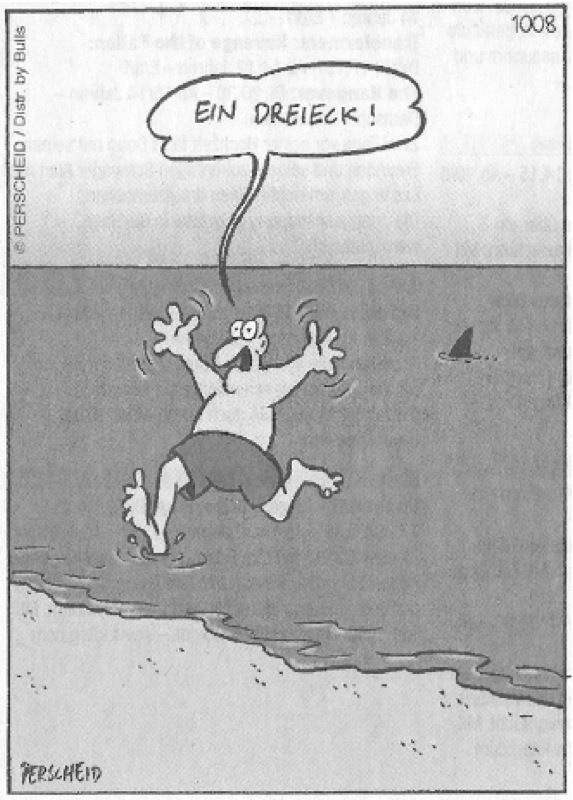
\includegraphics[width=0.618\textwidth]{pictures/dreiecksw.jpg}}
\title{Geometrie}
\subtitle{Rund um Ecken und Kanten}
\author{}
\date{}
%\lowertitleback{
%\includegraphics[height=1.1cm]{/Users/jormawassmer/Pictures/logokoeniz.jpg}%
%\copyright Jorma Wassmer
%1. Auflage, Februar 2011
%}


\begin{document}
\maketitle
\tableofcontents
%\thispagestyle{empty}
\cleardoublepage
%\setcounter{page}{1}

\section{Planimetrie}

\subsection{Testfragen Basics}
Welche der folgenden Aussagen sind richtig, welche falsch? Ist die Aussage richtig, dann versuche sie zu begr\"unden. Ist die Aussage falsch, dann gib ein Gegenbeispiel.
\begin{enumerate}
\item Zwei Geraden haben genau einen Schnittpunkt
\item Die Summe eines Winkels $\ga$ und seines Stufenwinkels betr\"agt $180^\circ $.
\item Die Winkelsumme im Dreieck betr\"agt $180^\circ $
\item Der $90^\circ $-Winkel kann konstruiert werden.
\item Der $15^\circ $-Winkel kann konstruiert werden.
\item Wird hintereinander an zwei verschiedenen Achsen gespiegelt, so erh\"alt man eine Verschiebung.
\item Eine Punktspiegelung entspricht einer Drehung um $180^\circ $.
\item Zwei Dreiecke sind kongruent, wenn sie in drei Seiten \"ubereinstimmen.
\item Die Innenwinkelsumme eines $n$-Ecks berechnet sich nach der Formel
$$2^{n-3}\cdot180^\circ .$$
\item Der Umkreismittelpunkt eines Dreiecks liegt im Innern des Dreiecks.
\item Halbieren sich die Diagonalen im einem Viereck, und besitzt das Viereck mindestens einen rechten Winkel, so handelt es sich um ein Rechteck.
\item Ein Parallelogramm ist ein spezielles Trapez.
\item Ein Rhombus besitzt gleich viele Symmetrieachsen wie ein gleichseitiges Dreieck.
\item Der Fl\"acheninhalt eines rechtwinkligen Dreiecks ($\gg=90^\circ $) ist
$$A=\frac{ab}{2}$$
\item Die Mittelsenkrechte einer Sehne eines Kreises geht durch den Mittelpunkt des Kreises.
\item Der Kreisbogen eines Kreises ist proportional zu seinem Zentriwinkel.
\item Der Fl\"acheninhalt eines Kreises ist proportional zu seinem Radius.
\item Die Mittellinie eines Trapezes ABCD mit den parallelen Seiten $a$ und $c$ hat die L\"ange
$$m=\frac{a+c}{2}$$
\item Die Peripheriewinkel \"uber einer Sehne sind alle gleich gross und halb so gross wie ihr Zentriwinkel.
\item Der Satz des Thales ist eine direkte Folgerung aus der oben genannten Feststellung.
\end{enumerate}
%Zum Satz von Thales gibt es im Appendix \ref{art:thales} einen lesenswerten Artikel.

\subsection{Konstruieren}
Man hält grundsätzlich an folgenden Konventionen fest:
\begin{itemize}
\item Konstruktionen sind mit Zirkel und Lineal durchzuf\"uhren.
\item Nicht konstruierbare Winkel misst man mit dem Geo-Dreieck (zB. $20^\circ $)
\item Zu Geometrieaufgaben geh\"oren im Allgemeinen eine Skizze und ein kurzer Kon\-struk\-tions\-bericht.
\end{itemize}

\setcounter{ueb}{20}
\begin{ueb}
Konstruiere Dreiecke aus folgenden Angaben:

\begin{minipage}{0.5\textwidth}
    \begin{enumeratea}
      %\item $a=\unit[6]{cm}$, $b=\unit[8]{cm}$, $c=\unit[7]{cm}$
      \item $c=\unit[5]{cm}$, $a=\unit[8]{cm}$, $\gb=40^\circ $
      \item $a=\unit[8]{cm}$, $\ga=50^\circ $, $\gb=70^\circ $
      \item $a=\unit[5]{cm}$, $b=\unit[8]{cm}$, $\ga=55^\circ $
      \item $a=\unit[7]{cm}$, $b=\unit[8]{cm}$, $\ga=55^\circ $
      \item $a=\unit[9]{cm}$, $b=\unit[8]{cm}$, $\ga=55^\circ $
    \end{enumeratea}
 \end{minipage}
 \begin{minipage}{0.4\textwidth}
 \begin{enumeratea}
 \setcounter{enumi}{5}
      %\item $a=\unit[5]{cm}$, $b=\unit[7]{cm}$, $h_c=\unit[4]{cm}$
      \item $\ga=60^\circ $, $b=\unit[4]{cm}$, $r=\unit[3]{cm}$
      \item $\ga=45^\circ $, $\gb=60^\circ $, $w_{\gb}=\unit[4]{cm}$
      \item $s_a=\unit[9]{cm}$, $s_b=\unit[6]{cm}$, $a=\unit[5]{cm}$
      \item $\ga=40^\circ $, $\gb=110^\circ $, $\rho=\unit[3]{cm}$
      \item $\ga=50^\circ $, $w_{\ga}=\unit[7]{cm}$, $\rho=\unit[2]{cm}$
    \end{enumeratea}
\end{minipage}
\end{ueb}

\subsection{Winkel am Kreis}
Es gilt bekanntlich folgender

\begin{csatz}[Peripheriewinkelsatz]{}
Der Peripheriewinkel \"uber einer Sehne $\overline{AB}$ ist halb so gross wie der zugeh\"orige Zentriwinkel.
\end{csatz}

\begin{proof}[Beweis]
Siehe \"Ubungen
\end{proof}

\begin{bem}
Aus dem Beweis folgt direkt, dass alle Peripheriewinkel \"uber gleichem Bogen gleich gross sind.
\end{bem}

\begin{figure}
\begin{center}
\definecolor{qqwuqq}{rgb}{0,0.39,0}
\definecolor{uququq}{rgb}{0.25,0.25,0.25}
\scalebox{0.618}{
\begin{tikzpicture}[line cap=round,line join=round,>=triangle 45,x=1.0cm,y=1.0cm]
\clip(-4.52,-4.38) rectangle (4.92,4.3);
\draw [shift={(2.41,3.19)},line width=1.6pt,color=qqwuqq,fill=qqwuqq,fill opacity=0.1] (0,0) -- (-142.7:0.8) arc (-142.7:-87.97:0.8) -- cycle;
\draw [shift={(0,0)},line width=1.6pt,color=qqwuqq,fill=qqwuqq,fill opacity=0.1] (0,0) -- (-158.3:0.8) arc (-158.3:-48.84:0.8) -- cycle;
\draw [line width=2pt] (0,0) circle (4cm);
\draw [line width=1.6pt] (-3.72,-1.48)-- (2.63,-3.01);
\draw [line width=1.6pt] (-3.72,-1.48)-- (2.41,3.19);
\draw [line width=1.6pt] (2.63,-3.01)-- (2.41,3.19);
\draw [line width=1.6pt] (0,0)-- (-3.72,-1.48);
\draw [line width=1.6pt] (0,0)-- (2.63,-3.01);
\begin{scriptsize}
\fill [color=uququq] (0,0) circle (1.5pt);
\draw[color=uququq] (0.18,0.26) node {$M$};
\fill [color=black] (-3.72,-1.48) circle (1.5pt);
\draw[color=black] (-4.08,-1.48) node {$A$};
\fill [color=black] (2.63,-3.01) circle (1.5pt);
\draw[color=black] (2.68,-3.36) node {$B$};
\fill [color=black] (2.41,3.19) circle (1.5pt);
\draw[color=black] (2.58,3.46) node {$C$};
\end{scriptsize}
\end{tikzpicture}
}
\end{center}
\caption{Peripheriewinkelsatz}
\end{figure}

\begin{ueb}
Berechne den Winkel $\epsilon$:
\begin{center}
\definecolor{qqwuqq}{rgb}{0,0.39,0}
\scalebox{0.618}{
\begin{tikzpicture}[line cap=round,line join=round,>=triangle 45,x=1.0cm,y=1.0cm]
\clip(-4.3,-4.04) rectangle (7.26,6.3);
\draw [shift={(165.88,139.34)},line width=1.6pt,color=qqwuqq] (0,0) -- (-161.06:1) arc (-161.06:-118.88:1) -- cycle;
\draw [shift={(-2.56,0.36)},line width=1.6pt,color=qqwuqq] (0,0) -- (-19.63:1) arc (-19.63:54.08:1) -- cycle;
\draw [line width=1.6pt] (0,0) circle (2.58cm);
\draw [line width=1.6pt,domain=-4.3:7.26] plot(\x,{(-17.32-2.17*\x)/-6.34});
\draw [line width=1.6pt,domain=-4.3:7.26] plot(\x,{(--17.32-5.87*\x)/-3.24});
\draw [line width=1.6pt] (-1.14,2.32)-- (-2.56,0.36);
\draw [line width=1.6pt] (-2.56,0.36)-- (2.21,-1.34);
\draw (4.86,4.4) node[anchor=north west] {$\epsilon$};
\draw (-2.2,0.75) node[anchor=north west] {$2\epsilon$};
\end{tikzpicture}
}
\end{center}
\end{ueb}

\begin{ueb}
Berechne den Winkel $\epsilon$:
\begin{center}
\definecolor{qqwuqq}{rgb}{0,0.39,0}
\definecolor{xdxdff}{rgb}{0.49,0.49,1}
\definecolor{uququq}{rgb}{0.25,0.25,0.25}
\scalebox{1.4}{
\begin{tikzpicture}[line cap=round,line join=round,>=triangle 45,x=1.0cm,y=1.0cm]
\clip(-1.72,-1.34) rectangle (4.78,5.06);
\draw [shift={(3,0)},line width=1.2pt,color=qqwuqq] (0,0) -- (108:1) arc (108:144:1) -- cycle;
\draw [line width=2pt] (1.5,2.06) circle (2.55cm);
\draw [line width=1.6pt] (1.5,4.62)-- (0,0);
\draw [line width=1.6pt] (0,0)-- (3.93,2.85);
\draw [line width=1.6pt] (3.93,2.85)-- (-0.93,2.85);
\draw [line width=1.6pt] (-0.93,2.85)-- (3,0);
\draw [line width=1.6pt] (3,0)-- (1.5,4.62);
\draw (-3,5.24) node[anchor=north west] {$\epsilon$};
\draw (2.48,0.7) node[anchor=north west] {$\epsilon$};
\draw (-0.48,4.74) node[anchor=north west] {$b$};
\draw (-1.28,1.28) node[anchor=north west] {b};
\draw (4.14,1.32) node[anchor=north west] {b};
\draw (3.28,4.52) node[anchor=north west] {b};
\draw (1.44,-0.66) node[anchor=north west] {b};
\begin{scriptsize}
\fill [color=uququq] (0,0) circle (1.5pt);
\fill [color=xdxdff] (3,0) circle (1.5pt);
\fill [color=uququq] (3.93,2.85) circle (1.5pt);
\fill [color=uququq] (1.5,4.62) circle (1.5pt);
\fill [color=uququq] (-0.93,2.85) circle (1.5pt);
\end{scriptsize}
\end{tikzpicture}
}
\end{center}
\end{ueb}

\begin{ueb}
Berechne den Winkel $\epsilon$:
\begin{center}
\definecolor{qqqqff}{rgb}{0,0,1}
\definecolor{qqwuqq}{rgb}{0,0.39,0}
\scalebox{1}{
\begin{tikzpicture}[line cap=round,line join=round,>=triangle 45,x=1.0cm,y=1.0cm]
\clip(-3.4,-3.58) rectangle (6.1,5.54);
\draw [shift={(1.1,5.16)},line width=1.2pt,color=qqwuqq] (0,0) -- (-118.96:1) arc (-118.96:-44.57:1) -- cycle;
\draw [shift={(1.16,1.16)},line width=1.2pt,color=qqwuqq] (0,0) -- (0:0.6) arc (0:90.86:0.6) -- cycle;
\draw [line width=1.6pt] (1.16,1.16) circle (4cm);
\draw [line width=1.6pt] (1.16,1.16)-- (5.16,1.16);
\draw [line width=1.6pt,dash pattern=on 5pt off 5pt] (1.1,5.16)-- (1.16,1.16);
\draw [shift={(1.24,-2.84)}] plot[domain=1.59:2.64,variable=\t]({1*4*cos(\t r)+0*4*sin(\t r)},{0*4*cos(\t r)+1*4*sin(\t r)});
\draw [line width=1.6pt] (1.1,5.16)-- (-2.26,-0.91);
\draw [line width=1.6pt] (1.1,5.16)-- (5.16,1.16);
\draw [line width=1.6pt,dotted] (1.16,1.16)-- (1.24,-2.84);
\draw [line width=1.6pt] (-2.27,-0.91)-- (5.16,1.12);
\draw (1.14,4.7) node[anchor=north west] {$\epsilon$};
\begin{scriptsize}
\fill [color=qqqqff] (1.44,1.4) circle (1.5pt);
\end{scriptsize}
\end{tikzpicture}
}
\end{center}
\end{ueb}
\begin{ueb}
Berechne den Winkel $\epsilon$:
\begin{center}
\definecolor{qqwuqq}{rgb}{0,0.39,0}
\scalebox{1}{
\begin{tikzpicture}[line cap=round,line join=round,>=triangle 45,x=1.0cm,y=1.0cm]
\clip(-4.38,-1.18) rectangle (5.26,5.02);
\draw [shift={(2.36,3.82)},line width=1.2pt,color=qqwuqq] (0,0) -- (-120.28:1) arc (-120.28:-75.26:1) -- cycle;
\draw [shift={(0.31,0.05)},line width=1.6pt]  plot[domain=-0.01:3.13,variable=\t]({1*4.29*cos(\t r)+0*4.29*sin(\t r)},{0*4.29*cos(\t r)+1*4.29*sin(\t r)});
\draw [line width=1.6pt] (-3.98,0.1)-- (4.6,0);
\draw [shift={(-3.98,0.1)},line width=1.6pt]  plot[domain=-0.01:0.53,variable=\t]({1*7.34*cos(\t r)+0*7.34*sin(\t r)},{0*7.34*cos(\t r)+1*7.34*sin(\t r)});
\draw [shift={(4.6,0)},line width=1.6pt]  plot[domain=2.1:3.13,variable=\t]({1*4.43*cos(\t r)+0*4.43*sin(\t r)},{0*4.43*cos(\t r)+1*4.43*sin(\t r)});
\draw [line width=1.6pt] (2.36,3.82)-- (3.36,0.01);
\draw [line width=1.6pt] (0.16,0.05)-- (2.36,3.82);
\draw [->,dash pattern=on 2pt off 2pt] (-3.98,0.1) -- (3.12,1.97);
\draw [->,dash pattern=on 2pt off 2pt] (4.6,0) -- (0.78,2.25);
\draw (2,3.3) node[anchor=north west] {$\epsilon$};
\end{tikzpicture}
}
\end{center}
\end{ueb}

\begin{ueb}
Konstruiere ein Parallelogramm aus den Diagonalen $\overline{AC}=5$ und $\overline{BD}=8$ sowie dem Winkel $\gb=50^\circ $.
\end{ueb}

\clearpage

\section{R\"aumliche Geometrie}

\begin{bem}
F\"arben Sie in den folgenden Figuren und Ihren Skizzen, soweit sinnvoll, die Geraden und Ebenen jeweils mit verschiedenen Farben.
\end{bem}

\subsection{Die Raumelemente Punkt, Gerade und Ebene}

\begin{center}
\definecolor{zzttqq}{rgb}{0.6,0.2,0}
\definecolor{qqqqff}{rgb}{0,0,1}
\begin{tikzpicture}[line cap=round,line join=round,>=triangle 45,x=0.5cm,y=0.5cm]
\clip(-2.12,-1.12) rectangle (14.58,5.28);
\fill[color=zzttqq,fill=zzttqq,fill opacity=0.1] (13,4.44) -- (8.04,4.44) -- (4.64,1) -- (10.62,1) -- cycle;
\draw [domain=-2.12:14.58] plot(\x,{(-2.71--4.24*\x)/4.22});
\draw [color=zzttqq] (13,4.44)-- (8.04,4.44);
\draw [color=zzttqq] (8.04,4.44)-- (4.64,1);
\draw [color=zzttqq] (4.64,1)-- (10.62,1);
\fill [color=qqqqff] (-0.74,2.92) circle (1.5pt);
\draw[color=qqqqff] (-1,3.3) node {$P$};
\draw[color=black] (0.22,0.32) node {$g$};
\draw[color=zzttqq] (5.7,1.5) node {$E$};
\end{tikzpicture}
\end{center}

Eine Gerade ist eindeutig durch zwei Punkte bestimmt. Man schreibt etwa $g=(A,B)$ f\"ur diejenige Gerade, welche durch die Punkte A und B geht.

\begin{ueb} \ \\[-4ex]
\begin{enumeratea}
\item Von den Punkten A, B, C, D liegen die ersten drei auf einer Geraden. Wie viele Geraden sind durch diese Punkte bestimmt?
\item Wie viele Geraden sind durch die Eckpunkte eines W\"urfels bestimmt?
\item Wie viele Geraden sind durch $n$ Punkte in allgemeiner Lage bestimmt?
\end{enumeratea}
\end{ueb}

\noindent Eine Ebene ist eindeutig bestimmt durch:
\begin{itemize}
\item drei Punkte, die nicht auf einer Geraden liegen (drei nicht kollineare Punkte)
\item eine Gerade und ein Punkte, der nicht auf ihr liegt
\item zwei sich schneidende Geraden
\item zwei parallele Geraden, die keinen gemeinsamen Punkt haben
\end{itemize}

\begin{ueb} \ \\[-4ex]
\begin{enumeratea}
\item Von $6$ Punkten liegen genau $5$ in einer Ebene. Wie viele Ebenen sind durch diese $6$ Punkte bestimmt?
\item Wie viele Ebenen sind durch die $8$ Eckpunkte eines W\"urfels bestimmt? Wie viele dieser Ebenen enthalten genau $4$, wie viele genau $3$ Eckpunkte?
\item Wie viele Ebenen sind durch $n$ Punkte in allgemeiner Lage bestimmt?
\item Wie viele Ebenen sind durch $n$ parallele Geraden im Raum im allgemeinen bestimmt?
\end{enumeratea}
\end{ueb}

\begin{ueb}
Gegeben ist ein Punkt P auf einer Geraden g im Raum. Ist die zu g senkrechte Gerade durch P eindeutig bestimmt?
\end{ueb}

\subsection{Geraden}

F\"ur die gegenseitige Lage zweier Geraden g und h im Raum sind vier F\"alle zu unterscheiden:
\begin{itemize}
\item g und h haben keinen Punkt gemeinsam, und es gibt eine Ebene, in der sie beide enthalten sind; g und h sind parallel, $g\cap h=\emptyset$.
\item g und h haben alle Punkte gemeinsam, d.h., sie sind identisch, $g=h$.
\item g und h haben genau einen Punkt gemeinsam, d.h., g und h schneiden sich, $g\cap h=\{S\}$.
\item g und h haben keinen gemeinsamen Punkt, und sie sind in keiner gemeinsamen Ebene enthalten, d.h., g und h sind zueinander windschief.
\end{itemize}

\begin{ueb}
Verbinden Sie vier nicht in einer Ebene liegende Punkte zu einem Viereck. Was l\"asst sich \"uber die Diagonalen sagen?
\end{ueb}
\begin{ueb}
Die Geraden g und h seien mit der Geraden s windschief. Sind dann g und h windschief?
\end{ueb}

\subsection{Gerade und Ebene}
F\"ur die gegenseitige Lage einer Geraden g und einer Ebene E sind drei F\"alle zu unterscheiden:
\begin{itemize}
\item g und E haben keinen gemeinsamen Schnittpunkt, d.h., g ist parallel zu E, $g\cap E=\emptyset$.
\item alle Punkte von g liegen in E, d.h., g liegt in E, g ist parallel zu E.
\item g und E haben genau einen gemeinsamen Punkt, d.h., g schneidet die Ebene E (Durchstosspunkt D), $g\cap E=\{D\}$
\end{itemize}

\begin{ueb}
g und h seien zwei zu einer Ebene E parallele Geraden. Welche Aussagen sind richtig:
\begin{enumeratea}
\item $g\| h$
\item $g\bot h$
\item $g\cap h=\emptyset$
\item g und h sind windschief
\item es l\"asst sich keine Aussage machen
\end{enumeratea}
\end{ueb}

\begin{ueb}
Die Ebenen $E_1$ und $E_2$ seien parallel ohne gemeinsamen Punkt. Wie liegt die Gerade $r$ zu $E_2$, wenn $r$
\begin{enumeratea}
\item parallel zu $E_1$ ist
\item $E_1$ schneidet
\item in $E_1$ liegt?
\end{enumeratea}
\end{ueb}

\subsection{Ebene und Ebene}
F\"ur die gegenseitige Lage zweier Ebenen $E_1$ und $E_2$ sind drei F\"alle zu unterscheiden.
\begin{itemize}
\item $E_1$ und $E_2$ haben keinen gemeinsamen Punkt; sie sind parallel, $E_1\cap E_2=\emptyset$.
\item $E_1$ und $E_2$ haben alle Punkte gemeinsam, d.h., sie sind identisch; $E_1=E_2$.
\item $E_1$ und $E_2$ haben eine Gerade gemeinsam, d.h. sie schneiden sich (Schnittgerade $s$); $E_1\cap E_2=\{s\}$
\end{itemize}

\begin{ueb}
Wie viele Schnittgeraden ergeben sich durch $n$ Ebenen in allgemeiner Lage?
\end{ueb}
\begin{ueb}
g und h seien windschiefe Geraden. Die Gerade s schneidet sowohl g als auch h. Wie viele Ebenen sind durch diese drei Geraden bestimmt?
\end{ueb}
\begin{ueb}
Die Geraden r und s seien windschief. R ist ein Punkt auf r, S ein Punkt auf s. Welches ist die Schnittgerade der Ebenen $E_1=(R,s)$ und $E_2=(S,r)$?
\end{ueb}

\begin{ueb}
Auf die Seiten eines W\"urfels wurden die Ziffern 1 bis 6 willk\"urlich verteilt. Kann man aus den beiden Ansichten des W\"urfels erkennen, welche Ziffer sich gegen\"uber der 1 befindet?
\begin{center}
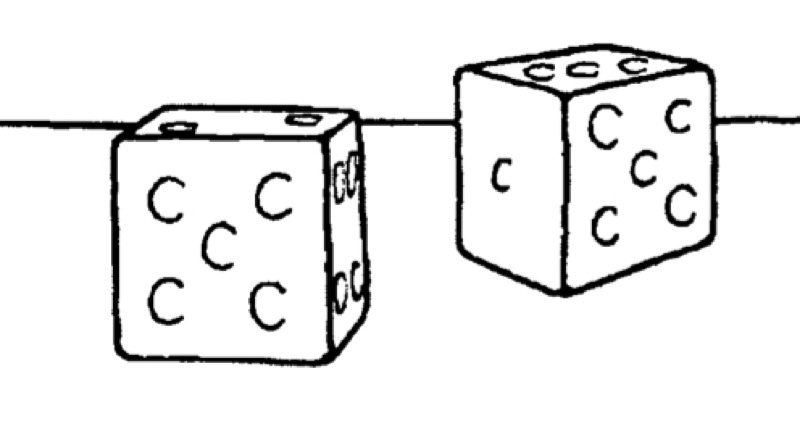
\includegraphics[width=7cm]{pictures/wuerfel}
\end{center}
\end{ueb}

\begin{ueb}
Kippe den W\"urfel aus dem mittleren Feld auf- oder abw\"arts, nach links oder rechts, jedoch nie diagonal. Nach sechs Kippbewegungen soll der W\"urfel mit der Augenzahl 6 nach oben auf dem Feld 1 liegen. Ist das mšglich?
\begin{center}
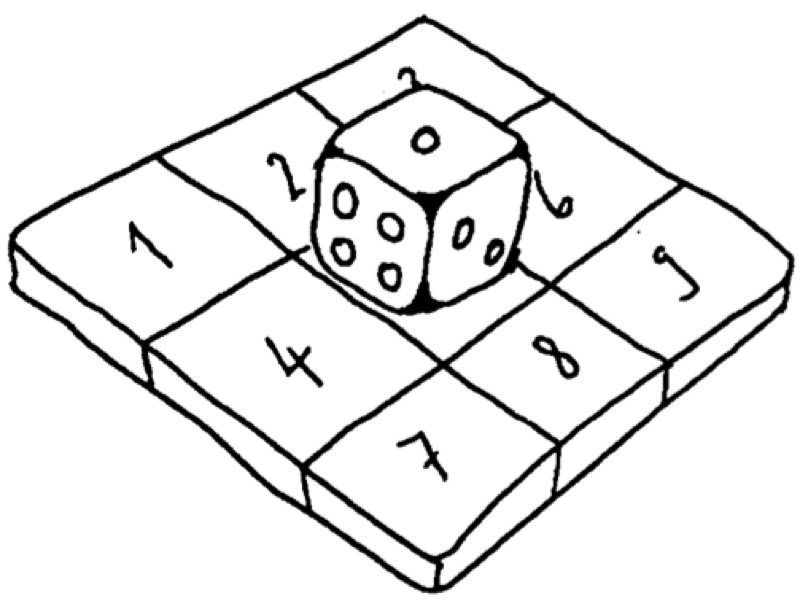
\includegraphics[width=7cm]{pictures/wuerfelfeld}
\end{center}
\end{ueb}

\subsection{Die Parallelprojektion von Geraden und Ebenen}
\begin{cdef}[Projektion]{}
Durch den Punkt $P$ wird ein Projektionsstrahl parallel zur Projektionsrichtung $r$ gelegt. Den Durchstosspunkt $P'$ mit der Bildebene nennt man das Bild oder die\emph{Projektion} von $P$.
\end{cdef}
\begin{center}
\definecolor{zzttqq}{rgb}{0.6,0.2,0}
\definecolor{xdxdff}{rgb}{0.49,0.49,1}
\definecolor{qqqqff}{rgb}{0,0,1}
\begin{tikzpicture}[line cap=round,line join=round,>=triangle 45,x=0.5cm,y=0.5cm]
\clip(-4.3,-1.06) rectangle (8.46,6.3);
\fill[color=zzttqq,fill=zzttqq,fill opacity=0.1] (6.12,0) -- (-4,0) -- (-2,3) -- (8,3) -- cycle;
\draw (8,3)-- (-2,3);
\draw (-2,3)-- (-4,0);
\draw (-4,0)-- (6,0);
\draw [->] (-4,6) -- (-2,4);
\draw (-1,6)-- (3,2);
\draw [dotted] (3,2)-- (5,0);
\draw (5,0)-- (6,-1);
\draw [color=zzttqq] (6.12,0)-- (-4,0);
\draw [color=zzttqq] (-4,0)-- (-2,3);
\draw [color=zzttqq] (-2,3)-- (8,3);
\draw[color=black] (-2.7,5.2) node {$r$};
\fill [color=qqqqff] (3,2) circle (1.5pt);
\draw[color=qqqqff] (3.3,2.5) node {$P'$};
\fill [color=qqqqff] (1,4) circle (1.5pt);
\draw[color=qqqqff] (1.3,4.5) node {$P$};
\draw[color=zzttqq] (-3,0.48) node {$E$};
\end{tikzpicture}
\end{center}

\begin{bem}
Die Sonnenstrahlen liefern ein anschauliches Modell paralleler Projektionsstrahlen.
\end{bem}

Durch jeden Punkt der Geraden g wird ein Projektionsstrahl gelegt. Diese Strahlen liegen in einer Ebene, der projizierenden Ebene.

Das Bild einer Geraden ist im allgemeinen wieder eine Gerade. Das Bild einer projizierenden Geraden ist ein Punkt.
\begin{cdef}[Spurpunkt]{}
Der Durchstosspunkt einer Geraden mit der Bildebene E heisst \emph{Spurpunkt} der Geraden.
\end{cdef}
Bilder von parallelen Geraden sind wieder parallel. Streckenverh\"altnisse bleiben bei der Projektion erhalten.

Das Bild einer Ebene ist im allgemeinen die ganze Bildebene. Das Bild einer projizierenden Ebene ist eine Gerade.
\begin{cdef}[Spur]{}
Die Schnittgerade einer Ebene mit der Bildebene E heisst \emph{Spur} der Ebene.
\end{cdef}

\subsection{Das r\"aumliche Koordinatensystem}
Wir legen einen W\"urfel auf die Zeichenebene (Bildebene) und projizieren ihn parallel auf die Zeichenebene. Die entstehende Parallelprojektion des W\"urfels ist eine zweidimensionale Darstellung des dreidimensionalen W\"urfels.
\begin{center}
\definecolor{qqqqff}{rgb}{0,0,1}
\scalebox{1.4}{
\begin{tikzpicture}[line cap=round,line join=round,>=triangle 45,x=1.0cm,y=1.0cm]
\clip(-4,-1.36) rectangle (4,5.5);
\draw [->] (-3.5,1) -- (3,1);
\draw [->] (-1,-1) -- (-1,5);
\draw [->] (1,2) -- (-4,-0.5);
\draw [line width=1.6pt] (-1,4)-- (-3,3);
\draw [line width=1.6pt] (-3,3)-- (-3,0);
\draw [line width=1.6pt] (-3,0)-- (0,0);
\draw [line width=1.6pt] (0,0)-- (2,1);
\draw [line width=1.6pt] (2,1)-- (2,4);
\draw [line width=1.6pt] (-1,4)-- (2,4);
\draw [line width=1.6pt] (-3,3)-- (0,3);
\draw [line width=1.6pt] (0,3)-- (2,4);
\draw [line width=1.6pt] (0,3)-- (0,0);
\draw[color=black] (3.1,1.2) node {$x$};
\draw[color=black] (-0.7,4.8) node {$y$};
\draw[color=black] (-3.8,-0.1) node {$z$};
\fill [color=qqqqff] (-3,3) circle (1.5pt);
\draw[color=qqqqff] (-2.84,3.4) node {$P'''$};
\fill [color=qqqqff] (0,0) circle (1.5pt);
\draw[color=qqqqff] (0.12,-0.3) node {$P'$};
\fill [color=qqqqff] (2,4) circle (1.5pt);
\draw[color=qqqqff] (2.2,4.3) node {$P''$};
\fill [color=qqqqff] (0,3) circle (1.5pt);
\draw[color=qqqqff] (0,3.3) node {$P$};
\end{tikzpicture}
}

xy-Ebene: Grundrissebene\\
yz-Ebene: Aufrissebene\\
xz-Ebene: Seitenrissebene\\
$P', P'', P'''$: Grund-, Auf-, Seitenriss von $P$
\end{center}
Die drei Koordinatenachsen werden aus den drei W\"urfelkanten gebildet, die in einer Ecke zusammenlaufen. Die y- und die z-Achse liegen in der Bildebene. Die x-Achse wird in die Bildebene projiziert und somit verzerrt.

Aus der Figur erkennt man, dass jeder Punkt $P$ des Raumes durch die Angabe dreier Koordinaten $x$, $y$ und $z$ eindeutig beschrieben werden kann. Man schreibt:
$$P\pointd{x}{y}{z}.$$

\begin{ueb}
Wo befinden sich die Figuren, die bei der zweidimensionalen Darstellung in wahrer Gršsse abgebildet werden?
\end{ueb}
\begin{ueb}
Zeichnen Sie die Raumbilder der folgenden Punkte:
$$A(-8|1|-3), B(4|3|1), C(3|-1|4), D(0|4|3).$$ Wie lauten die Koordinaten der drei Projektionen dieser Punkte?
\end{ueb}

\begin{ueb}
Zeichne das Schr\"agbild eines W\"urfels. Verbinde die Mittelpunkte der Seitenfl\"achen miteinander, um das Schr\"agbild eines Oktaeders zu erhalten.
\end{ueb}

\clearpage

\section{Stereometrie}
\begin{wrapfigure}{r}{0.382\textwidth}
  \begin{center}
    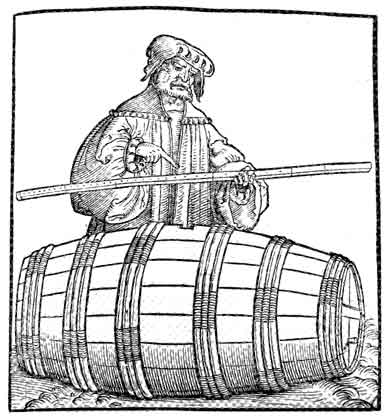
\includegraphics[width=0.382\textwidth]{pictures/fass}
  \end{center}
%\caption{A gull}
\end{wrapfigure}
Die Stereometrie (griech., K\"orpermessung) besch\"aftigt
sich im Gegensatz zur Planimetrie mit der Form, gegenseitigen Lage und Gr\"osse geometrischer Gebilde des Raumes. Im engeren Sinne ist sie die Lehre von der Ausmessung der K\"orper.

K\"orper sind Teile des Raumes, die durch ihre Oberfl\"ache vom \"ubrigen Raum abgegrenzt werden. K\"orper haben also ein bestimmtes Volumen und eine bestimmte Oberfl\"ache.
Die einfachen K\"orper --- W\"urfel, Quader, Zylinder, Kugel --- waren schon bei allen V\"olkern der vorgeschichtlichen Zeit bekannt und wurden praktisch genutzt (Hausbau, Fruchtspeicher, Gef\"asse, religi\"ose Zwecke etc.). Sowohl die Babyionier (3500 bis 200 v.u.Z.) als auch die \"Agypter (3000 bis 500 v.u.Z.) haben Volumen und Oberfl\"ache von W\"urfeln, Zylindern, Pyramiden, Pyramidenst\"umpfen, Kegeln und prismatischen K\"orpern, wenn auch teilweise nur in guter N\"aherung, berechnen k\"onnen. \textsc{Euklid} (350 v.u.Z.) f\"uhrte die ersten planm\"assigen, rein mathematischen Untersuchungen durch. Die Berechnung des Volumens und der Oberfl\"ache einer Kugel gelang aber erst Archimedes (287 - 212 v.u.Z.).

\subsection{Prismen}
\begin{ueb}
Berechne Volumen $V$, Oberfl\"ache $O$ und Raumdiagonale $d$ eines
\begin{enumeratea}
\item W\"urfels mit Kantenl\"ange $k$
\item eines Quaders mit Kantenl\"ange $a,b,c$
\end{enumeratea}
\end{ueb}

\subsection{Pyramiden}
\begin{ueb}
Die Cheopspyramide hat als Grundfl\"ache ein Quadrat mit Seitenl\"ange $\unit[233]{m}$. Sie war urspr\"unglich $\unit[148]{m}$ hoch; heute ist sie auf einer H\"ohe von $\unit[137]{m}$ abgestumpft.
\begin{enumeratea}
\item Der Bau soll $\unit[100000]{Mann}$ $\unit[20]{Jahre}$ besch\"aftigt haben. Welche Gesteinsmasse wurde dabei bewegt? (Dichte des Gesteins: $\rho_S=\unitfrac[2.7]{g}{cm^3}$)
\item Welche Abmessung hat die heutige Plattform?
\end{enumeratea}

\begin{figure}[h!]
\begin{center}
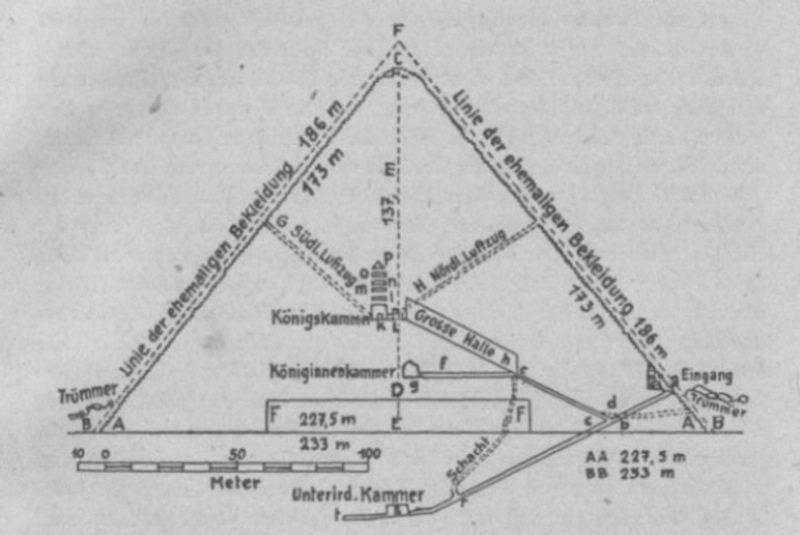
\includegraphics[width=0.9\textwidth]{pictures/cheops}
\caption{Cheopspyramide}
\end{center}
\end{figure}

\end{ueb}

\begin{ueb}
Ein Zelt hat die Gestalt eines regelm\"assigen sechsseitigen Pyramidenstumpfs mit den Grundkanten $a=\unit[4.8]{m}$ und $b=\unit[3.6]{m}$. Die Seitenkante misst jeweils $s=\unit[2.4]{m}$.
\begin{enumeratea}
\item Welchen Raum umschliesst das Zelt?
\item Wieviel Zeltstoff war zur Herstellung n\"otig?
\end{enumeratea}
\end{ueb}

\subsection{Gerader Kreiszylinder}
\begin{ueb}
Ein rechteckiges Blatt mit den Seitenl\"angen $a$ und $b$ kann auf zwei Arten zu einem Zylinder gebogen werden. Wie gross ist das Verh\"altnis der \\[1ex]
\hspace*{2.7ex}(a) Volumina$\q$ (b) M\"antel
\end{ueb}

\begin{ueb}
Eine Plakats\"aule ist $\unit[2.6]{m}$ hoch und hat einen Durchmesser von $\unit[1.2]{m}$. Wie gross ist die m\"ogliche Reklamefl\"ache?
\end{ueb}

\begin{ueb}
Wie viel Blech ben\"otigt man f\"ur eine Konservendose (Durchmesser $\unit[10]{cm}$, Inhalt $\unit[1]{Liter}$), wenn f\"ur Verschnitt etc. noch 15\% zugeschlagen werden?
\end{ueb}

\begin{ueb}
Eine Rolle Eisendraht (Dichte: $\unitfrac[7.8]{g}{cm^3}$) wiegt $\unit[135]{N}$. Wie lang ist der Draht, wenn seine Dicke $\unit[2.4]{mm}$ betr\"agt?
\end{ueb}

\begin{ueb}
Die Metallverkleidung eines Kamins muss mit einer Spezialfarbe zweimal gestrichen werden. Die Kaminverkleidung ist ein Zylinder mit einem Durchmesser von $\unit[150]{cm}$ und einer H\"ohe von $\unit[18]{m}$. Beim ersten Anstrich rechnet man mit $\unit[1]{kg}$ Farbe f\"ur $\unit[15]{m^2}$; beim zweiten Anstrich gen\"ugen 70\% der Menge des ersten Anstrichs. Wie viele Dosen (ˆ $\unit[5]{kg}$ bzw. $\unit[10]{kg}$) Farbe werden ben\"otigt?
\end{ueb}

\begin{ueb}
Zeichne die Parabel mit der Gleichung $y=4-x^2$ f\"ur $-2<x<2$. Lasse das Parabelst\"uck um die y-Achse rotieren, so dass ein Paraboloid entsteht, und berechne dessen Volumen. Hinweis: Betrachte einen Zylinder mit dem Radius 2 und der H\"ohe 4, aus dem ein kongruentes Rotationsparaboloid --- durch die Parabel $y=x^2$ entstanden --- herausgefr\"ast wird, und wende das Prinzip von Cavalieri an.
\end{ueb}

\subsection{Gerader Kreiskegel}
\begin{ueb}
Von einem geraden Kreiskegel kennt man den Radius $r=\unit[5]{cm}$ und das Volumen $V=\unit[1000]{cm^3}$. Berechne $h$, $s$, $M$ und $O$.
\end{ueb}

\begin{ueb}
Wie tief taucht ein Holzkegel ($r=\unit[5]{cm}$, $h=\unit[12]{cm}$, Dichte $\unitfrac[0.8]{g}{cm^3}$) mit der Spitze nach unten in Wasser ein?
\end{ueb}

\begin{ueb}
Wie gross ist der Mittelpunktswinkel des Kreisausschnittes, der den abgewickelten Mantel eines Kegels mit r=6 cm und h=8 cm darstellt?
\end{ueb}

\begin{ueb}
Ein Kreisausschnitt mit dem Mittelpunktswinkel 120¡ und dem Radius $\unit[8]{cm}$ wird zu einem Kegel zusammengebogen. Wie gross wird dessen Volumen?
\end{ueb}

\subsection{Kugel}
Die Berechnung des Volumens der Kugel erfolgt mit dem Prinzip von Cavalieri. Als Vergleichsk\"orper nimmt man denjenigen K\"orper, der entsteht, wenn man aus einem Zylinder (Radius $r$, H\"ohe $r$) einen Kegel herausfr\"ast.
Man schneidet die Halbkugel und den Vergleichsk\"orper mit einer Ebene, die vom Mittelpunkt der Kugel den Abstand $a$ hat. Als Schnittfl\"achen ergeben sich
f\"ur die Halbkugel
$$A = \pi r'^2 =\pi(r^2 - a^2),$$
f\"ur den Vergleichsk\"orper
$$A =A_{Kreisring} =\pi r^2-\pi a^2$$
F\"ur das Volumen der Kugel gilt deshalb:
\begin{align*}
V_{Halbkugel}&=V_{Zylinder}-V_{Kegel}\\
&=\pi r^3-\frac{1}{3}\pi r^3=\frac{2}{3}\pi r^3,
\end{align*}
also
$$V_{Kugel}=\frac{4}{3}\pi r^3.$$

\begin{ueb}
Berechne den Radius einer Kugel mit $\unit[1]{m^3}$ Rauminhalt.
\end{ueb}

\begin{ueb}
Leite eine Formel f\"ur das Materialvolumen einer Hohlkugel in Abh\"angigkeit vom Kugelradius rund der Wanddicke $d$ her. Welche Glieder der Formel k\"onnen bei sehr kleinem $d$ vernachl\"assigt werden? Deute die entstehende N\"aherungsformel und leite somit die Formel f\"ur die Oberfl\"ache einer Kugel ab.
\end{ueb}

\begin{ueb}
Der Inhalt der Gesamtaustauschfl\"ache der menschlichen Lunge betr\"agt ungef\"ahr $\unit[140]{m^2}$. Wie viele kugelf\"ormige (durchschnittlicher Durchmesser $\unit[0.3]{mm}$) Lungenbl\"aschen besitzt demnach ein Mensch?
\end{ueb}

\begin{ueb}
Wie verhalten sich die\\[1ex]
\hspace*{2.7ex}(a) Radien$\q$ (b) Oberfl\"achen$\q$ (c) Volumina\\[1ex]
der In- und Umkugel eines W\"urfels?
\end{ueb}

\begin{ueb}
Die Figur hat Archimedes in seinen Grabstein meisseln lassen.
\begin{center}
\definecolor{zzttqq}{rgb}{0.6,0.2,0}
\scalebox{0.85}{
\begin{tikzpicture}[line cap=round,line join=round,>=triangle 45,x=0.7cm,y=0.7cm]
\clip(-4.62,-2.54) rectangle (4.96,6.54);
\draw(0,2) circle (2.8cm);
\draw [color=zzttqq] (-4,6)-- (4,6);
\draw [color=zzttqq] (4,6)-- (4,-2);
\draw [color=zzttqq] (4,-2)-- (-4,-2);
\draw [color=zzttqq] (-4,-2)-- (-4,6);
\draw [color=zzttqq] (0,6)-- (-4,-2);
\draw [color=zzttqq] (-4,-2)-- (4,-2);
\draw [color=zzttqq] (4,-2)-- (0,6);
\end{tikzpicture}
}
\end{center}
Der R\"omer Cicero hat eineinhalb Jahrhunderte nach dem Tode von Archimedes dessen Grab an diesem Zeichen erkannt. Worauf soll dieses Zeichen wohl aufmerksam machen?
\end{ueb}

\begin{ueb}
Ein kugelf\"ormiger …ltropfen von $\unit[4]{mm}$ Durchmesser breitet sich auf einer Wasseroberfl\"ache zu einer Schicht von $\unit[1.2]{m^2}$ Fl\"acheninhalt aus. Berechne die H\"ohe dieser Schicht.
\end{ueb}

\clearpage

\section{Ähnlichkeit}

\subsection{Kongruenzabbildungen}
\begin{wrapfigure}{r}{0.382\textwidth}
  \begin{center}
    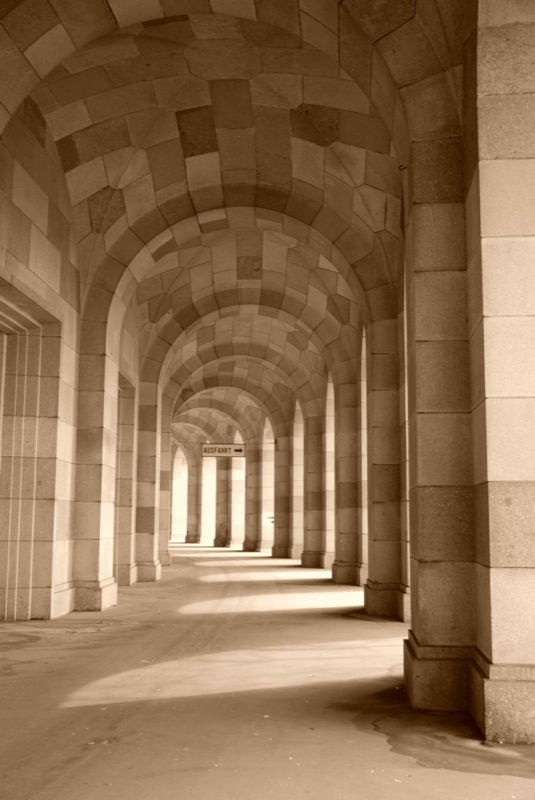
\includegraphics[width=0.382\textwidth]{pictures/torbogen}
  \end{center}
%\caption{A gull}
\end{wrapfigure}
Eine Abbildung ist eine eindeutige Zuordnung, bei der jedem Punkt einer ersten Punktmenge genau ein Punkt einer zweiten Punktmenge zugeordnet wird. Bei den Punktmengen handelt es sich um Geraden, Strecken, Winkel, Figuren (z.B. Dreiecke, Kreise), usw.

Wir nennen die erste Punktmenge die Originalmenge und die zweite Punktmenge die Bildmenge. In der Regel bezeichnen wir die Bildpunkte zu den Originalpunkten $A$, $B$, $P$, \dots\ mit $A'$, $B'$, $P'$, \dots.\\

Abbildungen, bei denen die Bildmenge deckungsgleich (kongruent) zur Originalmenge ist, heissen Kongruenzabbildungen. Kongruente Figuren haben also dieselbe Form und dieselbe Gr\"osse. Zu den Kongruenzabbildungen geh\"oren
\begin{itemize}
\item Achsenspiegelungen
\item Rotationen
\item Punktspiegelungen
\item Translationen
\item Verkettungen oben genannter Abbildungen
\end{itemize}

\begin{bsps}
\ \\[-2ex]
\begin{enumeratea}
\item Achsenspiegelung der Figur $F$ an der Geraden $g$%\\[4cm]
\item Drehung der Figur $F$ um den Drehpunkt $Z$ um den Winkel $\ga$%\\[5.5cm]
\item Punktspiegelung der Figur $F$ am Punkt $Z$%\\[6cm]
\item Verschiebung der Figur $F$ um einen vorgegebenen Verschiebungspfeil%\\[6cm]
\item Verkettung einer Achsenspiegelung mit einer Drehung
\end{enumeratea}
\end{bsps}

\subsection{Zentrische Streckung}
Wir w\"ahlen einen Punkt $Z$ der Ebene und eine positive Zahl $k$. Ordnen wir nun jedem Punkt $P$ einen Bildpunkt $P'$ zu gem\"ass der Vorschrift
\begin{itemize}
\item $P'$ liegt auf dem Strahl $ZP$
\item Die Strecke $ZP'$ ist $k$-mal so lang wie die Strecke $ZP$
\end{itemize}
so heisst diese Abbildung eine zentrische Streckung mit dem Streckungszentrum $Z$ und dem Streckungfaktor $k$.%\\[7cm]

F\"ur $k>1$ ist das Bild gr\"osser als das Original, f\"ur $k=1$ sind Bild und Original identisch und f\"ur $0<k<1$ ist das Bild kleiner als das Original.

\begin{bsp} Gegeben sind ein Punkt $Z$ und ein Dreieck $ABC$. Das Dreieck ist von $Z$ aus mit dem Streckungsfaktor $2$ zentrisch zu strecken.%\\[6cm]
\end{bsp}
Eine zentrische Streckung hat folgende Eigenschaften
\begin{itemize}
\item Originalwinkel und Bildwinkel sind gleich gross.
\item Originalgerade und Bildgerade sind parallel.
\item Die Bildstrecke ist $k$-mal so lang wie die Originalstrecke.
\item Der Fl\"acheninhalt der Bildfigur ist $k^2$-mal so gross wie der Fl\"acheninhalt der Originalfigur.
\end{itemize}

\begin{ueb}
Strecken Sie ein Quadrat $Q$ von einem Punkt $Z$ aus mit dem Streckungsfaktor $3$ zentrisch und \"uberpr\"ufe anschliessend obige Eigenschaften.%\\[8cm]
\end{ueb}

\begin{ueb}
Eine Streckung mit einem negativen Streckungsfaktor bedeutet eine Streckung mit dem entgegengesetzten positiven Streckungsfaktor und eine zus\"atzliche Punktspiegelung am Streckungszentrum.

\noindent Strecke ein Dreieck von $Z$ aus mit dem Streckungsfaktor $-\frac{1}{2}$.
\end{ueb}

\subsection{\"Ahnlichkeitsabbildungen}
Kongruenzabbildungen, zentrische Streckungen und ihre Verkettungen heissen \"Ahnlichkeitsabbildungen. Figuren, welche durch \"Ahnlichkeitsabbildungen auseinander hervorgehen, heissen zueinander \"ahnlich. \"Ahnliche Figuren haben dieselbe Form.

\begin{bsp}
Verkettung einer Drehung mit einer zentrischen Streckung.%\\[7cm]
\end{bsp}

Eine \"Ahnlichkeitsabbildung hat folgende Eigenschaften
\begin{itemize}
\item Originalwinkel und Bildwinkel sind gleich gross.
\item Alle Bildstrecken sind $k$-mal so lang wie die entsprechenden Originalstrecken.
\item Der Fl\"acheninhalt der Bildfigur ist $k^2$-mal so gross wie der Fl\"acheninhalt der Originalfigur
\end{itemize}
Daraus folgt insbesondere f\"ur \"ahnliche Dreiecke, dass sie gleiche Winkel haben und im Verh\"altnis von zwei einander entsprechenden Seiten \"ubereinstimmen.

\begin{ueb}
Alle Kreise sind zueinander \"ahnlich. Wie verhalten sich die Fl\"achen zweier Kreise, wenn sich ihre Radien wie $2\div3$ verhalten? Gib ein konkretes Beispiel zweier solcher Kreise.
\end{ueb}

\subsection{Strahlens\"atze}
\begin{csatz}[1. Strahlensatz]{}
Werden zwei Strahlen mit gemeinsamem Anfangspunkt von zwei Parallelen geschnitten, so verhalten sich die Abschnitte auf dem einen Strahl wie die entsprechenden Abschnitte auf dem andern Strahl.%\\[6cm]
\end{csatz}

\begin{bsp}
Standardbeispiel mit $a=25$, b=$10$ und $c=32$. Bestimme den fehlenden Abschnitt $d$.%\\[6cm]
\end{bsp}

\begin{ueb}
Teile eine Strecke im Verh\"altnis $2\div3$.
\end{ueb}

\begin{csatz}[2. Strahlensatz]{}
Werden zwei Strahlen mit gemeinsamem Anfangspunkt von zwei Parallelen geschnitten, so verhalten sich die Parallelenabschnitte wie die vom Anfangspunkt aus gemessenen Abschnitte auf einem der Strahlen.%\\[6cm]
\end{csatz}

\begin{bsp}
Standardbeispiel mit $a=8$, $b=3$ und $p=10$. Bestimme $q$.%\\[6cm]
\end{bsp}

\begin{ueb}
Eine freistehende Telefonstange im ebenen Gel\"ande wirft bei einem bestimmten Sonnenstand einen Schatten von $\unit[5.6]{m}$ L\"ange. Um die Stangenh\"ohe $h$ zu bestimmen, wird ein Meterstab parallel zur Stange aufgestellt, so dass beide Schattengrenzen zusammenfallen. Der Abstand des Meterstabes von der Stange misst $\unit[2.9]{m}$.
\end{ueb}

Beide Strahlens\"atze gelten sinngem\"ass auch dann, wenn \dots
\begin{itemize}
\item \dots\ mehr als zwei Strahlen von zwei Parallelen geschnitten werden.
\item \dots\ zwei Strahlen von mehr als zwei Parallelen geschnitten werden.
\item \dots\ anstatt Strahlen zwei sich schneidende Geraden von zwei Parallelen geschnitten werden.
\end{itemize}

\begin{bsp}
Ein Fotograf steht in der Entfernung $e=\unit[60]{m}$ von einem Baum. Die Brennweite $f$ des Kamera-Objektivs betr\"agt $\unit[45]{mm}$, die Gr\"osse $a$ des Baum-Bildes auf dem Negativ misst $\unit[24]{mm}$. Berechne die Baumh\"ohe $h$.%\\[7cm]
\end{bsp}
Alle Strahlens\"atze lassen sich z.B. mit Hilfe von \"ahnlichen Dreiecken beweisen.

\subsection{\"Ahnliche K\"orper}
K\"orper, welche durch \"Ahnlichkeitsabbildungen auseinander hervorgehen, heissen zueinander \"ahnlich. \"Ahnliche K\"orper haben dieselbe Form.

Neben den bereits bekannten Eigenschaften von \"Ahnlichkeitsabbildungen
\begin{itemize}
\item Eine Bildstrecke ist $k$-mal so lang wie die entsprechende Originalstrecke.
\item Der Fl\"acheninhalt einer Bildfigur ist $k^2$-mal so lang wie der Fl\"acheninhalt der entsprechenden Originalfigur.
\end{itemize}
gilt zus\"atzlich
\begin{itemize}
\item Das Volumen de Bildk\"orpers ist $k^3$-mal so gross wie das Volumen des Originalk\"orpers%\\[6cm]
\end{itemize}

\begin{bsp}
Alle W\"urfel sind zueinander \"ahnlich.\\

\definecolor{wwwwww}{rgb}{0.4,0.4,0.4}
\begin{center}
\scalebox{1}{
\begin{tikzpicture}[line cap=round,line join=round,>=triangle 45,x=0.8259911894273128cm,y=0.6036217303822938cm]
\draw [color=wwwwww,dash pattern=on 2pt off 2pt, xstep=0.5cm,ystep=0.5cm] (-4.3,-3.8) grid (13.3,6.3);
\clip(-4.3,-3.64) rectangle (13.86,6.3);
\end{tikzpicture}
}
\end{center}
\end{bsp}

\begin{bsps}
\ \\[-2ex]
\begin{enumeratea}
\item Zwei W\"urfel aus gleichem Material wiegen $\unit[1]{g}$ und $\unit[1]{kg}$. Der leichtere W\"urfel hat eine Kantenl\"ange von $\unit[5]{cm}$. Wie lang ist eine Kante des schwereren W\"urfels?

Weil die beiden W\"urfel aus gleichem Material sind verhalten sich wegen
$$\frac{m_1}{m_2}=\frac{V_1\cdot\rho}{V_2\cdot\rho}=\frac{V_1}{V_2}$$
ihre Volumina wie $1\div1000$, also wegen $10^3=1000$ ihre Kantenl\"angen wie $1\div10$. Die Kantenl\"ange des schwereren W\"urfels betr\"agt deshalb $\unit[50]{cm}$.
\item Ein gerader Kreiskegel wird durch einen Schnitt parallel zur Grundfl\"ache in halber H\"ohe geteilt. Er zerf\"allt dabei in einen kleineren Kegel und einen Kegelstumpf. Wie verhalten sich die Volumina der beiden Teile?

Der kleine Kegel ist zum urspr\"unglichen \"ahnlich (zentrische Streckung mit Kegelspitze als Streckungszentrum). Ihre H\"ohne verhalten sich wie $1\div2$, ihre Grundfl\"achen wie $1\div4$ und ihre Volumina wie $1\div8$. Das Volumen des Kegelstumpfs ist Volumen des urspr\"unglichen Kegels minus Volumen des kleinen Kegels. Also verh\"alt sich das Volumen des kleinen Kegels zu dem des Kegelstumpfs wie $1\div7$.
\end{enumeratea}
\end{bsps}

\clearpage

\subsection{\"Ubungen}
\begin{enumerate}
\item Spiegle das Dreieck und den Kreis an der Geraden $g$.\\
\begin{center}
\scalebox{1.3}{
\begin{tikzpicture}[line cap=round,line join=round,>=triangle 45,x=0.7cm,y=0.7cm]
\clip(-4.22,-3.2) rectangle (6.84,5.64);
\draw [line width=1.6pt,domain=-4.22:6.84] plot(\x,{(--18.3-3.62*\x)/10.7});
\draw [line width=2pt] (0.96,1.39)-- (-0.58,5.4);
\draw [line width=2pt] (-0.58,5.4)-- (-0.72,1.1);
\draw [line width=2pt] (-0.72,1.1)-- (0.96,1.39);
\draw [line width=1.6pt] (3.6,-1.7) circle (0.8cm);
\draw[color=black] (-3.24,2.36) node {$g$};
\fill [color=black] (3.6,-1.7) circle (1.5pt);
\end{tikzpicture}
}
\end{center}
\item Die Figur $F$ kann durch eine Achsenspiegelung in die Figur $F'$ \"uberf\"uhrt werden. Konstruiere die Spiegelachse.\\
\begin{center}
\scalebox{1.2}{
\begin{tikzpicture}[line cap=round,line join=round,>=triangle 45,x=1cm,y=1cm]
\clip(-3.17,-2.47) rectangle (4.08,2.91);
\draw [line width=1.6pt] (-1.98,-1.86)-- (-2.22,-0.14);
\draw [line width=1.6pt] (-2.22,-0.14)-- (0.64,-2.18);
\draw [line width=1.6pt] (3.33,1.56)-- (1.86,2.49);
\draw [line width=1.6pt] (1.86,2.49)-- (2.54,-0.96);
\draw (-2.79,-0.69) node[anchor=north west] {$F'$};
\draw (3.1,2.3) node[anchor=north west] {$F$};
\end{tikzpicture}
}
\end{center}



\item Spiegle das Rechteck $ABCD$ an der Rechteckdiagonalen durch $A$ und $C$.\\
\begin{center}
\scalebox{1.2}{
\begin{tikzpicture}[line cap=round,line join=round,>=triangle 45,x=0.9cm,y=0.9cm]
\clip(-2.66,-2.21) rectangle (3.98,1.08);
\draw [line width=2pt] (-1.87,-1.32)-- (2.91,-1.32);
\draw [line width=2pt] (2.91,-1.32)-- (2.86,0.52);
\draw [line width=2pt] (2.86,0.52)-- (-1.87,0.48);
\draw [line width=2pt] (-1.87,0.48)-- (-1.87,-1.32);
\draw (-2.1,-1.4) node[anchor=north west] {$A$};
\draw (2.6,-1.4) node[anchor=north west] {$B$};
\draw (2.6,1) node[anchor=north west] {$C$};
\draw (-2.1,1) node[anchor=north west] {$D$};
\end{tikzpicture}
}
\end{center}

\item Geht eine Figur durch eine Achsenspiegelung in sich selbst \"uber, so heisst die Figur achsensymmetrisch. Bei Achsensymmetrie heisst die Spiegelachse auch Symmetrieachse der Figur.

Zeichne bei den Figuren alle m\"oglichen Symmetrieachsen und Symmetriepunkte ein.\\
\begin{center}
\scalebox{1.1}{
\begin{tikzpicture}[line cap=round,line join=round,>=triangle 45,x=0.9cm,y=0.75cm]
\clip(-4.7,-0.9) rectangle (8,2.84);
\draw [line width=2pt] (-4,2)-- (-1,2);
\draw [line width=2pt] (-1,2)-- (-1,0);
\draw [line width=2pt] (-1,0)-- (-4,0);
\draw [line width=2pt] (-4,0)-- (-4,2);
\draw [line width=2pt] (1,-0.5)-- (1,1.5);
\draw [line width=2pt] (1,1.5)-- (4,2.5);
\draw [line width=2pt] (4,2.5)-- (4,0.5);
\draw [line width=2pt] (4,0.5)-- (1,-0.5);
\draw [line width=2pt] (5,2)-- (7,2);
\draw [line width=2pt] (7,2)-- (7,0);
\draw [line width=2pt] (7,0)-- (5,0);
\draw [line width=2pt] (5,0)-- (5,2);
\end{tikzpicture}
}
\end{center}
\item Drehe den Punkt $P$ um $Z$ um den Winkel $120^\circ$ im Uhrzeigersinn.\\[4cm]
\begin{center}
\scalebox{1.1}{
\begin{tikzpicture}[line cap=round,line join=round,>=triangle 45,x=1.368cm,y=1.368cm]
\clip(-2.66,-0.56) rectangle (3.92,1.08);
\fill [color=black] (-1.39,0.3) circle (1.5pt);
\draw[color=black] (-1.27,0.52) node {$P$};
\fill [color=black] (1.67,0.25) circle (1.5pt);
\draw[color=black] (1.78,0.47) node {$Z$};
\end{tikzpicture}
}
\end{center}
\item Drehe die Figur im Gegenuhrzeigersinn um $Z$ um den Winkel $\ga$.\\
\begin{center}
\definecolor{qqwuqq}{rgb}{0,0.39,0}
\scalebox{0.95}{
\begin{tikzpicture}[line cap=round,line join=round,>=triangle 45,x=1.0817369093231162cm,y=1.0783987915407858cm]
\clip(-2.66,-4.39) rectangle (10.28,1.08);
\draw [shift={(9.42,-2.04)},line width=1pt,color=qqwuqq] (0,0) -- (130.66:0.83) arc (130.66:226.37:0.83) -- cycle;
\draw [line width=2pt] (0.94,-0.62)-- (-1.04,-2.21);
\draw [line width=2pt] (-1.04,-2.21)-- (0.48,-3.25);
\draw [line width=2pt] (0.48,-3.25)-- (0.94,-0.62);
\draw (8.31,-0.76)-- (9.42,-2.04);
\draw (8.41,-3.1)-- (9.42,-2.04);
\fill [color=black] (3.01,-1.32) circle (1.5pt);
\draw[color=black] (3.12,-1.1) node {$Z$};
\draw[color=qqwuqq] (8.9,-2) node {$\alpha$};
\end{tikzpicture}
}
\end{center}

\item Die Aufnahme zeigt den n\"achtlichen Nordhimmel. Wegen der langen Belichtungszeit haben die Sterne kreisbogenf\"ormige Spuren hinterlassen, deren Mittelpunkt den Himmelspol kennzeichnet. Die dicke Spur unterhalb des Drehzentrums stammt vom Polarstern.

Wie lange wurde der Film belichtet?\\
\begin{center}
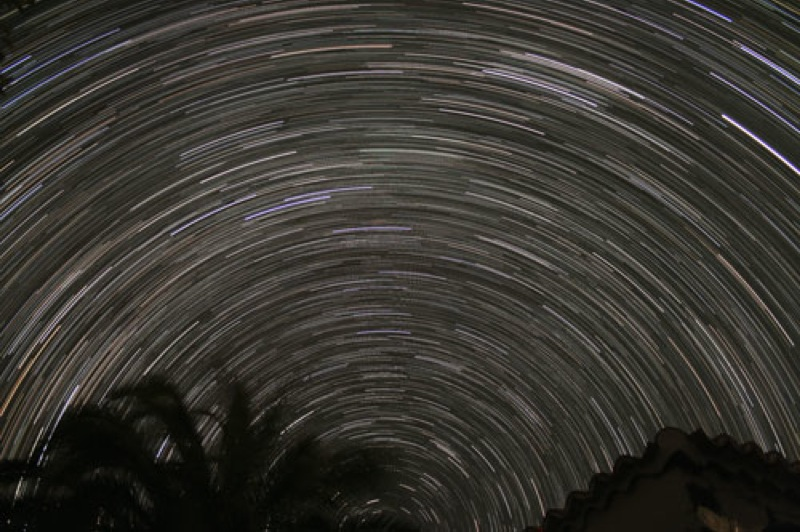
\includegraphics[width=0.92\textwidth]{pictures/ueb7}
\end{center}

\pagebreak

\item Der Punkt $A$ wurde um einen Drehpunkt nach $A'$ gedreht. Wo muss der Drehpunkt liegen?
\begin{center}
\scalebox{1}{
\begin{tikzpicture}[line cap=round,line join=round,>=triangle 45,x=0.7974481658692185cm,y=0.7943925233644861cm]
\clip(-4.3,2.02) rectangle (8.24,6.3);
\fill [color=black] (-2,3) circle (1.5pt);
\draw[color=black] (-1.84,3.4) node {$A$};
\fill [color=black] (4.56,3.84) circle (1.5pt);
\draw[color=black] (4.74,4.26) node {$A'$};
\end{tikzpicture}
}
\end{center}

\item Die Strecke $AB$ wurde um einen Drehpunkt nach $A'B'$ gedreht. Konstruiere den Drehpunkt.\\
\begin{center}
\scalebox{0.8}{
\begin{tikzpicture}[line cap=round,line join=round,>=triangle 45,x=0.75cm,y=0.75cm]
\clip(-4.3,-1.54) rectangle (7.86,6.3);
\draw [line width=2pt] (-2.16,0.22)-- (-0.42,3.98);
\draw [line width=2pt] (6.1,0.82)-- (3.58,4.1);
\draw (-2.8,0.8) node[anchor=north west] {$A$};
\draw (-0.9,4.68) node[anchor=north west] {$B$};
\draw (3.68,4.8) node[anchor=north west] {$A'$};
\draw (6.26,1.24) node[anchor=north west] {$B'$};
\end{tikzpicture}
}
\end{center}

\item Eine rechteckige Tischplatte soll auf ihrem Untergestell derart gelagert sein, dass sie die beiden gezeichneten Lagen einnehmen kann. An welcher Stelle muss der Tischler den Drehzapfen anbringen?\\
\begin{center}
\begin{tikzpicture}[line cap=round,line join=round,>=triangle 45,x=0.75cm,y=0.75cm]
\clip(-3.96,-0.84) rectangle (5.4,6.72);
\draw [line width=2pt] (-3,0)-- (3,0);
\draw [line width=2pt] (3,0)-- (3,2);
\draw [line width=2pt] (3,2)-- (-3,2);
\draw [line width=2pt] (-3,2)-- (-3,0);
\draw [line width=2pt,dash pattern=on 4pt off 4pt] (-1,6)-- (1,6);
\draw [line width=2pt,dash pattern=on 4pt off 4pt] (1,6)-- (1,0);
\draw [line width=2pt,dash pattern=on 4pt off 4pt] (1,0)-- (-1,0);
\draw [line width=2pt,dash pattern=on 4pt off 4pt] (-1,0)-- (-1,6);
\end{tikzpicture}
\end{center}

\pagebreak

\item Drehe die Figur um $Z$ um $180^\circ$.\\
\begin{center}
\begin{tikzpicture}[line cap=round,line join=round,>=triangle 45,x=0.8cm,y=0.8cm]
\clip(-3.76,-0.28) rectangle (4.86,5.12);
\draw [line width=2pt] (-2.22,4.54)-- (-3.42,0.46);
\draw [line width=2pt] (-3.42,0.46)-- (0.6,0.48);
\draw [line width=2pt] (0.6,0.48)-- (-0.1,3.58);
\draw [line width=2pt] (-0.1,3.58)-- (-2.22,4.54);
\fill [color=black] (4.14,1) circle (1.5pt);
\draw[color=black] (4.4,1.3) node {$Z$};
\end{tikzpicture}
\end{center}
\item Verschiebe das Dreieck um den vorgegebenen Verschiebungspfeil.\\[3ex]
\begin{center}
\scalebox{0.95}{
\begin{tikzpicture}[line cap=round,line join=round,>=triangle 45,x=0.79cm,y=0.79cm]
\clip(-3.76,-1.46) rectangle (8.92,5.12);
\draw [line width=2pt] (7.04,3.22)-- (7.68,-0.52);
\draw [line width=2pt] (7.68,-0.52)-- (5.5,-0.94);
\draw [line width=2pt] (5.5,-0.94)-- (7.04,3.22);
\draw [->] (7.04,3.22) -- (1.22,4.4);
\end{tikzpicture}
}
\end{center}

\item Das Viereck $V$ kann durch eine Verschiebung in $V'$ \"uberf\"uhrt werden. Zeichne einen zugeh\"origen Verschiebungspfeil.\\
\begin{center}
\scalebox{0.8}{
\begin{tikzpicture}[line cap=round,line join=round,>=triangle 45,x=1.0cm,y=1.0cm]
\clip(-2.6,-2.3) rectangle (7.28,3.58);
\draw [line width=2pt] (-1.38,1.02)-- (1.8,1.02);
\draw [line width=2pt] (1.8,1.02)-- (1.2,3.2);
\draw [line width=2pt] (1.2,3.2)-- (-0.72,2.7);
\draw [line width=2pt] (-0.72,2.7)-- (-1.38,1.02);
\draw [line width=1.6pt] (2.68,-1.24)-- (5.86,-1.24);
\draw [line width=1.6pt] (5.86,-1.24)-- (5.26,0.94);
\draw [line width=1.6pt] (5.26,0.94)-- (3.34,0.44);
\draw [line width=1.6pt] (3.34,0.44)-- (2.68,-1.24);
\draw (0.2,2.42) node[anchor=north west] {$V$};
\draw (4.28,0.1) node[anchor=north west] {$V'$};
\end{tikzpicture}
}
\end{center}

\pagebreak

\item Verschieben Sie das Dreieck zuerst um den ersten, dann um den zweiten angegebenen Verschiebungspfeil. Zeichnen Sie anschliessend einen Verschiebungspfeil, durch den das Originaldreieck direkt in die Endlage \"uberf\"uhrt wird.\\[-4ex]
\begin{center}

\begin{tikzpicture}[line cap=round,line join=round,>=triangle 45,x=0.94cm,y=0.94cm]
\clip(-4.3,0.12) rectangle (6.3,6.3);
\draw [line width=2pt] (-3.6,3.52)-- (-0.5,3.04);
\draw [line width=1.6pt] (-0.5,3.04)-- (-3.36,1.8);
\draw [line width=1.6pt] (-3.36,1.8)-- (-3.6,3.52);
\draw [->,line width=1pt] (-0.5,3.04) -- (4.8,3.82);
\draw [->,line width=1pt] (4.8,3.82) -- (5.16,2);
\end{tikzpicture}
\end{center}
\item Ein Sportflugzeug fliegt mit einer Geschwindigkeit von $\unitfrac[240]{km}{h}$ nach Norden. Von Westen weht ein Wind mit $\unitfrac[60]{km}{h}$. Bestimmen Sie an der Abbildung die Richtung und die tats\"achliche Geschwindigkeit des Flugzeugs gegen\"uber dem Erdboden.\\
\begin{center}
\scalebox{0.95}{
\begin{tikzpicture}[line cap=round,line join=round,>=triangle 45,x=1.04cm,y=1.04cm]
\clip(-1.12,-0.16) rectangle (1.76,4.3);
\draw [->,line width=1.6pt] (0,0) -- (1,0);
\draw [->,line width=1.6pt] (0,0) -- (0,4);
\draw (0.1,4) node[anchor=north west] {$\unitfrac[240]{km}{h}$};
\draw (0.4,0.7) node[anchor=north west] {$\unitfrac[60]{km}{h}$};
\end{tikzpicture}
}
\end{center}

\item Zwei Schlepper ziehen an einem Frachtschiff mit den Kr\"aften $F_1$ bzw.~$F_2$. Zeichne die resultierende Kraft, durch welche das Schiff bewegt wird.\\
\begin{center}
\definecolor{zzttqq}{rgb}{0.6,0.2,0}
\scalebox{0.7}{
\begin{tikzpicture}[line cap=round,line join=round,>=triangle 45,x=1.25cm,y=1.25cm]
\clip(-1.62,-1.18) rectangle (3.96,1.82);
\fill[color=zzttqq,fill=zzttqq,fill opacity=0.1] (-1.44,1.18) -- (-0.38,1.2) -- (-0.36,0.28) -- (-1.44,0.28) -- cycle;
\draw [->,line width=2pt] (0.88,0.78) -- (2.9,1.2);
\draw [->,line width=2pt] (0.88,0.78) -- (3.2,-0.48);
\draw (2.08,1.8) node[anchor=north west] {$F_1$};
\draw (2.3,-0.3) node[anchor=north west] {$F_2$};
\draw [shift={(-1.03,-2.21)},line width=2pt]  plot[domain=0.83:1.68,variable=\t]({1*3.95*cos(\t r)+0*3.95*sin(\t r)},{0*3.95*cos(\t r)+1*3.95*sin(\t r)});
\draw [shift={(-0.68,3)},line width=2pt]  plot[domain=4.46:5.5,variable=\t]({1*3.24*cos(\t r)+0*3.24*sin(\t r)},{0*3.24*cos(\t r)+1*3.24*sin(\t r)});
\draw [color=zzttqq] (-1.44,1.18)-- (-0.38,1.2);
\draw [color=zzttqq] (-0.38,1.2)-- (-0.36,0.28);
\draw [color=zzttqq] (-0.36,0.28)-- (-1.44,0.28);
\end{tikzpicture}
}
\end{center}

\pagebreak

\item Ein Schiff f\"ahrt bei einem Nordostwind von $\unitfrac[40]{km}{h}$ mit der Geschwindigkeit $\unitfrac[25]{km}{h}$ nach S\"uden. Von welcher Seite scheint f\"ur einen an Deck stehenden Passagier der Wind zu kommen und welche Geschwindigkeit scheint er zu haben? L\"ose die Aufgabe zeichnerisch.
\item Durch zentrische Streckung mit dem Streckungszentrum $Z$ ist aus dem Originaldreieck $ABC$ das Bilddreieck $A'B'C'$ entstanden.

Mit welchem Streckungsfaktor wurde es gestreckt? In welchem Verh\"altnis stehen entsprechende Seitenl\"angen zueinander? In welchem Verh\"altnis stehen die Fl\"acheninhalte zueinander?\\[-6ex]
\begin{center}
\definecolor{zzttqq}{rgb}{0.6,0.2,0}
\definecolor{wwttqq}{rgb}{0.4,0.2,0}
\definecolor{qqwwcc}{rgb}{0,0.4,0.8}
\definecolor{qqqqzz}{rgb}{0,0,0.6}
\begin{tikzpicture}[line cap=round,line join=round,>=triangle 45,x=0.865cm,y=0.865cm]
\clip(-1.62,-4.9) rectangle (9.94,1.82);
\fill[color=qqwwcc,fill=qqwwcc,fill opacity=0.1] (1.14,-1.62) -- (2.58,-1.92) -- (2.04,-2.58) -- cycle;
\fill[color=zzttqq,fill=zzttqq,fill opacity=0.1] (4.86,-0.66) -- (9.18,-1.56) -- (7.56,-3.54) -- cycle;
\draw [line width=2.4pt,color=qqwwcc] (1.14,-1.62)-- (2.58,-1.92);
\draw [line width=2.8pt,color=qqwwcc] (2.58,-1.92)-- (2.04,-2.58);
\draw [line width=2.4pt,color=qqwwcc] (2.04,-2.58)-- (1.14,-1.62);
\draw [domain=-0.72:9.94] plot(\x,{(-3.56--0.48*\x)/1.86});
\draw [domain=-0.72:9.94] plot(\x,{(-6.8--0.18*\x)/3.3});
\draw [domain=-0.72:9.94] plot(\x,{(-6.14-0.48*\x)/2.76});
\draw [line width=2.4pt,color=zzttqq] (4.86,-0.66)-- (9.18,-1.56);
\draw [line width=2.4pt,color=zzttqq] (9.18,-1.56)-- (7.56,-3.54);
\draw [line width=2.4pt,color=zzttqq] (7.56,-3.54)-- (4.86,-0.66);
\fill [color=black] (-0.72,-2.1) circle (1.5pt);
\draw[color=black] (-0.92,-1.7) node {$Z$};
\fill [color=qqqqzz] (1.14,-1.62) circle (1.5pt);
\draw[color=qqqqzz] (1.18,-1.26) node {$C$};
\fill [color=qqqqzz] (2.58,-1.92) circle (1.5pt);
\draw[color=qqqqzz] (2.72,-1.66) node {$B$};
\fill [color=qqqqzz] (2.04,-2.58) circle (1.5pt);
\draw[color=qqqqzz] (1.88,-2.86) node {$A$};
\fill [color=wwttqq] (4.86,-0.66) circle (1.5pt);
\draw[color=wwttqq] (5,-0.3) node {$C'$};
\fill [color=wwttqq] (9.18,-1.56) circle (1.5pt);
\draw[color=wwttqq] (9.36,-1.3) node {$B'$};
\fill [color=wwttqq] (7.56,-3.54) circle (1.5pt);
\draw[color=wwttqq] (7.44,-3.86) node {$A'$};
\end{tikzpicture}
\end{center}
\item Strecke die Figur von $Z$ aus mit dem Streckungsfaktor $\frac{1}{3}$.\\
\begin{center}
\definecolor{zzttqq}{rgb}{0.6,0.2,0}
\scalebox{1.1}{
\begin{tikzpicture}[line cap=round,line join=round,>=triangle 45,x=0.865cm,y=0.865cm]
\clip(-1.62,-4.9) rectangle (9.94,1.82);
\fill[color=zzttqq,fill=zzttqq,fill opacity=0.1] (-1.02,-2.56) -- (-0.98,-4.7) -- (5.1,-4.74) -- (5.1,-4.02) -- (-0.16,-4.02) -- (-0.2,-2.56) -- cycle;
\draw [color=zzttqq] (-1.02,-2.56)-- (-0.98,-4.7);
\draw [color=zzttqq] (-0.98,-4.7)-- (5.1,-4.74);
\draw [color=zzttqq] (5.1,-4.74)-- (5.1,-4.02);
\draw [color=zzttqq] (5.1,-4.02)-- (-0.16,-4.02);
\draw [color=zzttqq] (-0.16,-4.02)-- (-0.2,-2.56);
\draw [color=zzttqq] (-0.2,-2.56)-- (-1.02,-2.56);
\fill [color=black] (8.92,0.9) circle (1.5pt);
\draw[color=black] (8.7,1.26) node {$Z$};
\end{tikzpicture}
}
\end{center}

\pagebreak

\item Strecke das Rechteck von $Z$ aus mit dem Streckungsfaktor $-2$.\\
\begin{center}
\definecolor{zzttqq}{rgb}{0.6,0.2,0}
\definecolor{zzzzzz}{rgb}{0.6,0.6,0.6}
\scalebox{0.9}{
\begin{tikzpicture}[line cap=round,line join=round,>=triangle 45,x=0.93cm,y=0.93cm]
\draw [color=zzzzzz,dash pattern=on 2pt off 2pt, xstep=0.93cm,ystep=0.93cm] (0.56,-6.52) grid (15.62,1.4);
\clip(0.56,-6.52) rectangle (15.62,1.4);
\fill[color=zzttqq,fill=zzttqq,fill opacity=0.1] (3,0) -- (7,0) -- (7,-2) -- (3,-2) -- cycle;
\draw [color=zzttqq] (3,0)-- (7,0);
\draw [color=zzttqq] (7,0)-- (7,-2);
\draw [color=zzttqq] (7,-2)-- (3,-2);
\draw [color=zzttqq] (3,-2)-- (3,0);
\fill [color=black] (7,-2) circle (1.5pt);
\draw[color=black] (6.8,-2.32) node {$Z$};
\end{tikzpicture}
}
\end{center}
\item Das Dreieck $ABC$ kann durch eine zentrische Streckung in das Bilddreieck $A'B'C'$ \"uberf\"uhrt werden. Konstruiere das Streckungszentrum $Z$ und gib den Streckungsfaktor an.\\
\begin{center}
\definecolor{uququq}{rgb}{0.25,0.25,0.25}
\definecolor{zzttqq}{rgb}{0.6,0.2,0}
\definecolor{wwwwww}{rgb}{0.4,0.4,0.4}
\scalebox{0.9}{
\begin{tikzpicture}[line cap=round,line join=round,>=triangle 45,x=1.1cm,y=1.1cm]
\draw [color=wwwwww,dash pattern=on 3pt off 3pt, xstep=1.1cm,ystep=1.1cm] (0.56,-6.78) grid (14.28,1.4);
\clip(0.56,-6.78) rectangle (14.28,1.4);
\draw [line width=2pt,color=zzttqq] (3,-5)-- (10,-5);
\draw [line width=2pt,color=zzttqq] (10,-5)-- (5,-1);
\draw [line width=2pt,color=zzttqq] (5,-1)-- (3,-5);
\draw [line width=2pt] (2,-5.5)-- (12.5,-5.5);
\draw [line width=2pt] (12.5,-5.5)-- (5,0.5);
\draw [line width=2pt] (5,0.5)-- (2,-5.5);
\fill [color=zzttqq] (3,-5) circle (1.5pt);
\draw[color=zzttqq] (2.98,-5.26) node {$A$};
\fill [color=zzttqq] (10,-5) circle (1.5pt);
\draw[color=zzttqq] (9.98,-5.26) node {$B$};
\fill [color=zzttqq] (5,-1) circle (1.5pt);
\draw[color=zzttqq] (5.24,-0.82) node {$C$};
\fill [color=uququq] (2,-5.5) circle (1.5pt);
\draw[color=uququq] (2,-5.84) node {$A'$};
\fill [color=uququq] (12.5,-5.5) circle (1.5pt);
\draw[color=uququq] (12.52,-5.82) node {$B'$};
\fill [color=uququq] (5,0.5) circle (1.5pt);
\draw[color=uququq] (5.38,0.64) node {$C'$};
\end{tikzpicture}
}
\end{center}

\pagebreak

\item Verbindet man die Seitenmitten eines Dreiecks $ABC$, so entsteht ein weiteres Dreieck. Dieses k\"onnte aus dem Dreieck $ABC$ durch eine zentrische Streckung erhalten werden. Wo liegt das Streckungszentrum und wie gross ist der Streckungsfaktor?

\item Der Eckpunkt $B$ des Dreiecks $ABC$ wurde durch eine zentrische Streckung von $Z$ aus in $B'$ \"uberf\"uhrt. Konstruiere das Bilddreieck $A'B'C'$, und bestimme den Streckungsfaktor.\\
\begin{center}
\definecolor{uququq}{rgb}{0.25,0.25,0.25}
\definecolor{zzttqq}{rgb}{0.6,0.2,0}
\scalebox{0.95}{
\begin{tikzpicture}[line cap=round,line join=round,>=triangle 45,x=0.9336cm,y=0.9336cm]
\clip(0.56,-9.62) rectangle (10.2,1.4);
\draw [line width=2pt,color=zzttqq] (9,-3)-- (2,1);
\draw [line width=2pt,color=zzttqq] (2,1)-- (3,-3);
\draw [line width=2pt,color=zzttqq] (3,-3)-- (9,-3);
\draw (2,1)-- (2,-9);
\fill [color=black] (9,-3) circle (1.5pt);
\draw[color=black] (9.2,-3.28) node {$A$};
\fill [color=black] (2,1) circle (1.5pt);
\draw[color=black] (1.68,1.12) node {$B$};
\fill [color=black] (3,-3) circle (1.5pt);
\draw[color=black] (3.02,-3.32) node {$C$};
\fill [color=black] (2,-9) circle (1.5pt);
\draw[color=black] (1.68,-9.12) node {$Z$};
\fill [color=uququq] (2,-5) circle (1.5pt);
\draw[color=uququq] (1.66,-5.02) node {$B'$};
\end{tikzpicture}
}
\end{center}

\pagebreak

\item Gegeben sei ein Trapez mit den parallelen Seiten $a=\unit[7]{cm}$ und $c=\unit[4]{cm}$. Verl\"angern Sie die Schenkel bis sie sich schneiden und bezeichnen Sie den Schnittpunkt mit $Z$. Bei einer zentrischen Streckung von $Z$ aus soll die Strecke $c$ das Bild der Strecke $a$ sein; wie gross ist der Streckungsfaktor?\\
\begin{center}
\scalebox{0.8}{
\begin{tikzpicture}[line cap=round,line join=round,>=triangle 45,x=1.057cm,y=1.057cm]
\clip(0.98,-5.88) rectangle (10.44,1.02);
\draw [line width=2pt] (9,-5)-- (8,-3);
\draw [line width=2pt] (8,-3)-- (5,-3);
\draw [line width=2pt] (5,-3)-- (2,-5);
\draw [line width=2pt] (2,-5)-- (9,-5);
\draw[color=black] (6.5,-2.62) node {$c$};
\draw[color=black] (5.36,-5.26) node {$a$};
\end{tikzpicture}
}
\end{center}

\item In einem Zimmer steht das schwarze rechteckige Brett parallel zur Wand auf dem Boden. Von einem Punkt vom Boden aus strahlt Licht. Zeichnen Sie die Lichtstrahlen durch die oberen Eckpunkte des Bretts und finde so deren Schlagschatten an der Wand.\\
\begin{center}
\definecolor{zzttqq}{rgb}{0.6,0.2,0}
\definecolor{ccccqq}{rgb}{0.8,0.8,0}
\scalebox{0.9}{
\begin{tikzpicture}[line cap=round,line join=round,>=triangle 45,x=0.9124cm,y=0.9124cm]
\clip(2.22,-7.84) rectangle (13.18,-0.04);
\fill[fill=black,fill opacity=1.0] (6.9,-4.34) -- (7.58,-5.47) -- (7.6,-4.28) -- (6.86,-3.22) -- cycle;
\fill[color=zzttqq,fill=zzttqq,fill opacity=0.1] (9.5,-3.44) -- (11.2,-5.8) -- (7.58,-5.47) -- (7.6,-4.28) -- (7.5,-4.13) -- cycle;
\draw (2.54,-6.8)-- (11.92,-6.8);
\draw (11.92,-6.8)-- (11.84,-0.5);
\draw (11.92,-6.8)-- (8.54,-2.12);
\draw (8.54,-2.12)-- (8.56,-0.58);
\draw (8.54,-2.12)-- (4.14,-2.1);
\draw (4.46,-5.18)-- (11.2,-5.8);
\draw (4.46,-5.18)-- (9.5,-3.44);
\draw (6.9,-4.34)-- (7.58,-5.47);
\draw (7.58,-5.47)-- (7.6,-4.28);
\draw (7.6,-4.28)-- (6.86,-3.22);
\draw (6.86,-3.22)-- (6.9,-4.34);
\draw [color=zzttqq] (9.5,-3.44)-- (11.2,-5.8);
\draw [color=zzttqq] (11.2,-5.8)-- (7.58,-5.47);
\draw [color=zzttqq] (7.58,-5.47)-- (7.6,-4.28);
\draw [color=zzttqq] (7.6,-4.28)-- (7.5,-4.13);
\draw [color=zzttqq] (7.5,-4.13)-- (9.5,-3.44);
\fill [color=ccccqq] (4.46,-5.18) circle (1.5pt);
\end{tikzpicture}
}
\end{center}
\item Ein Filmnegativ der Gr\"osse $\unit[24\times36]{mm}$ soll so vergr\"ossert werden, dass das Bild alles zeigt, was auf dem Negativ ist. Bei welchem der drei Papierformate $9\times13$, $10\times15$, $13\times18$ (alle Masse in $\unit{cm}$) ist dies ohne Verschnitt m\"oglich?
\item Auf dem Kartenausschnitt links ist das Kilometernetz erkennbar. Damit l\"asst sich der Kartenmassstab bestimmen. Ermittle daraus den Massstab der Luftaufnahme rechts.\\
\begin{center}
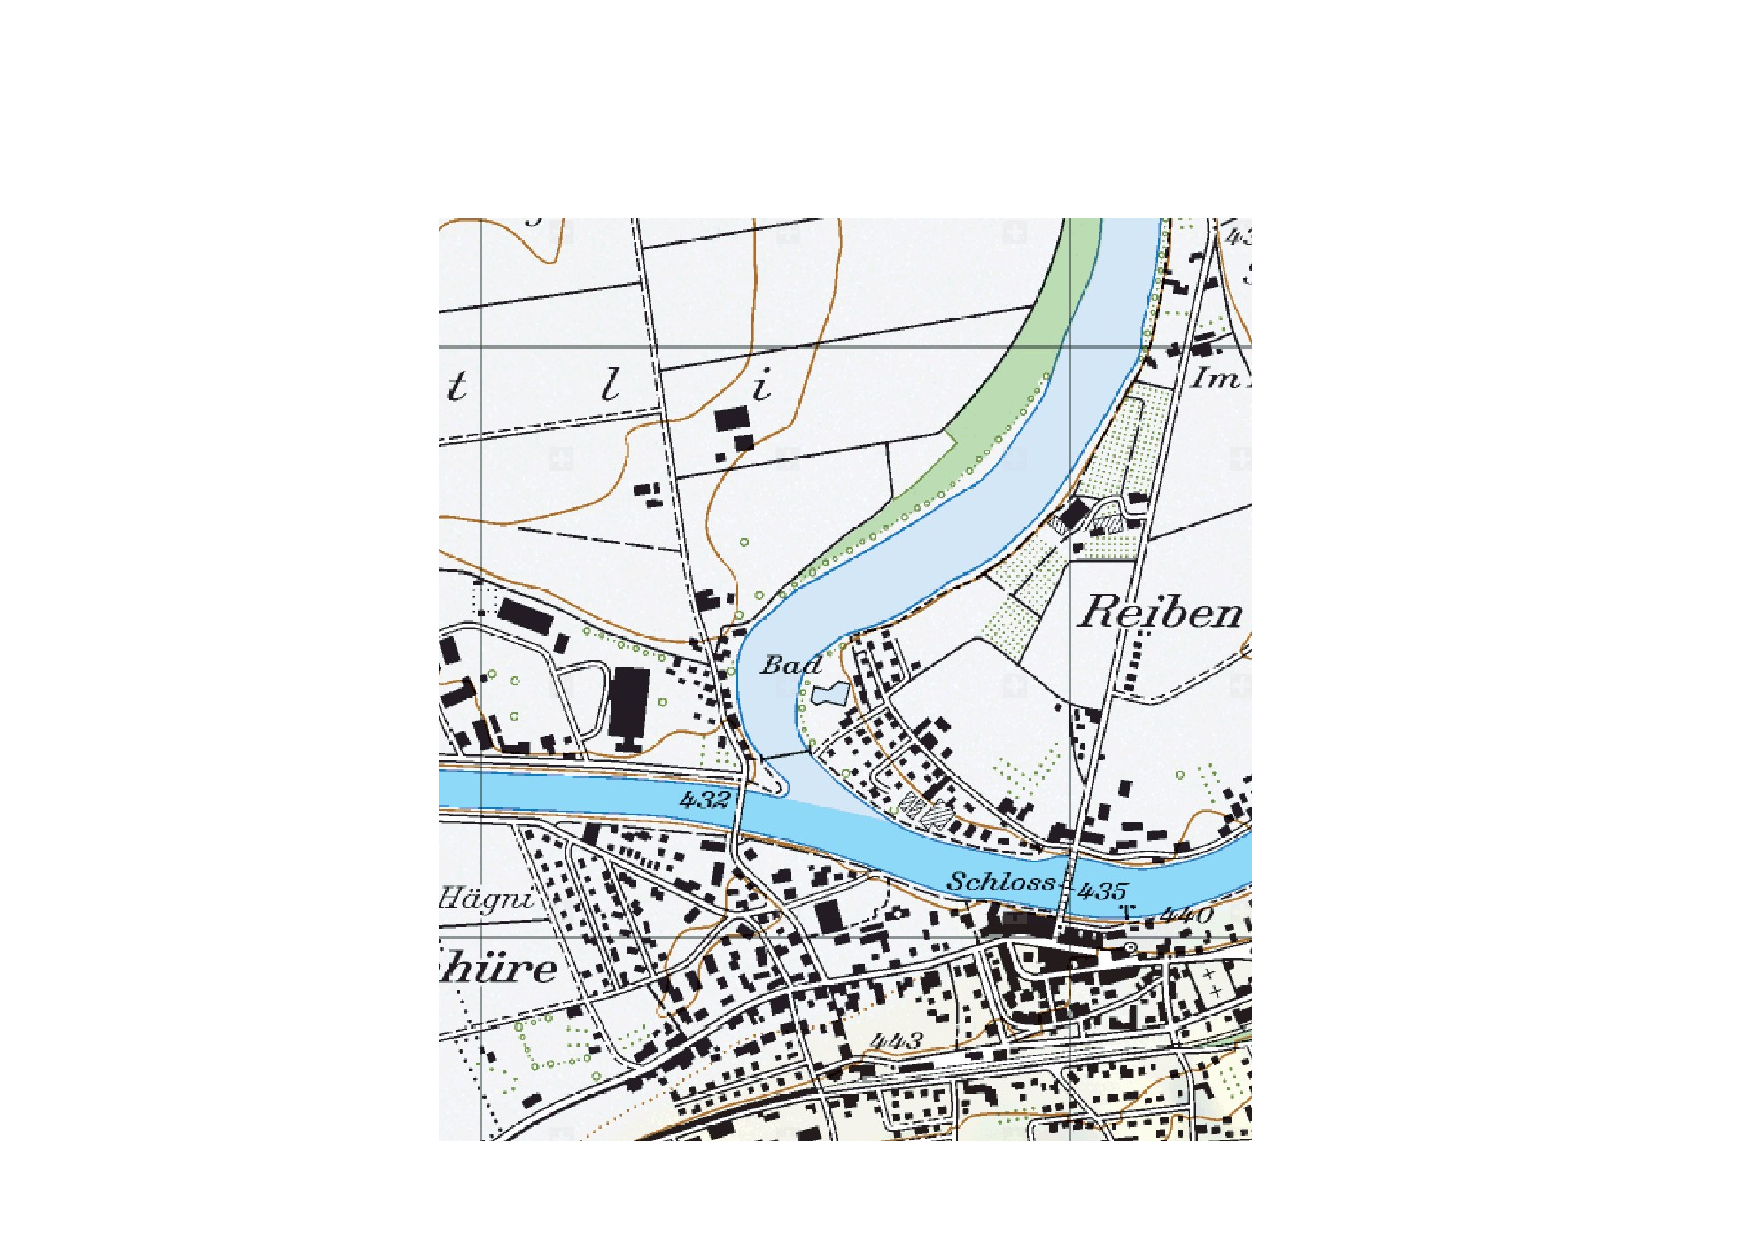
\includegraphics[width=7cm]{pictures/burenmap.pdf}\hspace*{0.2cm}
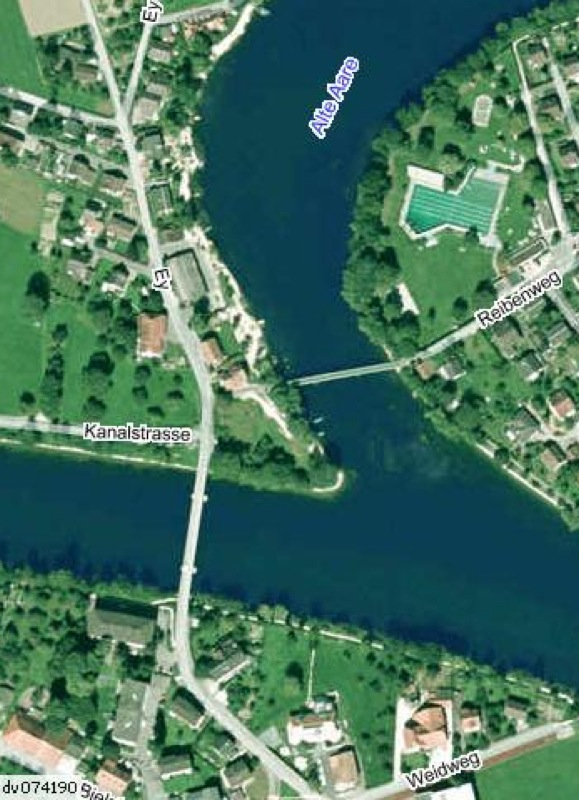
\includegraphics[width=7cm]{pictures/ueb27lb}
\end{center}

\item Der Kreis mit Mittelpunkt $M$ soll von $Z$ aus so gestreckt werden, dass der Bildkreis die Gerade $g$ ber\"uhrt. Konstruiere den Bildkreis.
\begin{center}
\definecolor{qqqqff}{rgb}{0,0,1}
\scalebox{0.9}{
\begin{tikzpicture}[line cap=round,line join=round,>=triangle 45,x=0.7353cm,y=0.7353cm]
\clip(0.52,-6.76) rectangle (16.84,0.36);
\draw [line width=1.6pt] (7.54,-0.4)-- (16.12,-3.18);
\draw [line width=1.6pt] (6.42,-3.68) circle (1.47cm);
\fill [color=black] (6.42,-3.68) circle (1.5pt);
\draw[color=black] (6.16,-3.96) node {$M$};
\fill [color=qqqqff] (0.94,-1.8) circle (1.5pt);
\draw[color=qqqqff] (0.72,-1.4) node {$Z$};
\end{tikzpicture}
}
\end{center}
\item Bei einer zentrischen Streckung eines Kreises vervierfacht sich dessen Radius. Wie ver\"andert sich dabei der Inhalt der Kreisfl\"ache?
\item Bei einer zentrischen Streckung eines Quadrats wird dessen Fl\"acheninhalt $100$ mal gr\"osser. Wie viel mal gr\"osser wird dabei die Seitenl\"ange?
\item Ein Mikroskop vergr\"ossert $100$-fach. Wie viel mal wird mit diesem Mikroskop der Fl\"acheninhalt eines Insektenfl\"ugels vergr\"ossert?
\item Auf einer Karte mit Massstab $1\div25'000$ ist ein horizontales Autobahnst\"uck $\unit[65]{mm}$ lang und eine Stadt bedeckt eine Fl\"ache von $\unit[420]{cm^2}$. Wie lang ist das Autobahnst\"uck und wie gross ist die Stadtfl\"ache in Wirklichkeit?
\item Die Schweiz hat eine Fl\"ache von $\unit[41'000]{km^2}$. Die Luftlinie Bern-Thun betr\"agt $\unit[25]{km}$. Welche Fl\"ache hat die Schweiz auf einer Karte, bei der die Distanz Bern-Thun $\unit[5]{cm}$ betr\"agt?
\item Die Skizze zeigt ein dreieckiges Segel $ABC$, das um eine Stange gewickelt werden kann. Dabei verkleinert sich die Segelfl\"ache auf die gestrichelte Gr\"osse.
\begin{center}
\scalebox{0.8}{
\begin{tikzpicture}[line cap=round,line join=round,>=triangle 45,x=1cm,y=1cm]
\clip(0.52,-4.6) rectangle (6.82,0.36);
\draw [line width=1.6pt] (2.12,-0.24)-- (5.34,-2.86);
\draw [line width=1.6pt] (5.34,-2.86)-- (2.16,-3.34);
\draw [line width=4pt] (2.12,-0.24)-- (2.16,-3.34);
\draw [line width=1.6pt,dash pattern=on 5pt off 5pt] (2.13,-1.12)-- (3.82,-2.48);
\draw [line width=1.6pt,dash pattern=on 5pt off 5pt] (3.82,-2.48)-- (2.15,-2.68);
\draw (1.68,-3.46) node[anchor=north west] {A};
\draw (5.64,-2.76) node[anchor=north west] {B};
\draw (1.5,0.04) node[anchor=north west] {C};
\end{tikzpicture}
}
\end{center}
\begin{enumeratea}
\item Ein Segel von $\unit[20]{m^2}$ Fl\"acheninhalt wird soweit aufgerollt, bis die Segelunterkante $AB$ von $\unit[5]{m}$ auf $\unit[4]{m}$ verk\"urzt wird. Wie gross ist die neue Segelfl\"ache?
\item Ein $\unit[36]{m^2}$ grosses Segel wird auf $\unit[16]{m^2}$ verkleinert. Um welchen Faktor verkleinert sich die Segelunterkante $AB$?
\end{enumeratea}

\pagebreak

\item Die Originalfigur $A$ kann je durch eine \"Ahnlichkeitsabbildung in die Bildfigur $B$, $C$, $D$, $E$, $F$ oder $G$ abgebildet werden.
\begin{center}
\definecolor{zzttqq}{rgb}{0.6,0.2,0}
\definecolor{wwwwww}{rgb}{0.4,0.4,0.4}
\scalebox{0.7}{
\begin{tikzpicture}[line cap=round,line join=round,>=triangle 45,x=1cm,y=1cm]
\draw [color=wwwwww,dash pattern=on 2pt off 2pt, xstep=0.5cm,ystep=0.5cm] (-4.3,-5.24) grid (10.2,6.3);
\clip(-4.3,-5.24) rectangle (10.42,6.3);
\fill[color=zzttqq,fill=zzttqq,fill opacity=0.1] (-3.5,5.5) -- (-0.5,5.5) -- (-0.5,3.5) -- (-1.5,3.5) -- (-1.5,4.5) -- (-3.5,4.5) -- cycle;
\fill[color=zzttqq,fill=zzttqq,fill opacity=0.1] (3.5,3.5) -- (3.5,5.5) -- (6.5,5.5) -- (6.5,4.5) -- (4.5,4.5) -- (4.5,3.5) -- cycle;
\fill[color=zzttqq,fill=zzttqq,fill opacity=0.1] (0.5,2.5) -- (2.5,2.5) -- (2.5,-0.5) -- (1.5,-0.5) -- (1.5,1.5) -- (0.5,1.5) -- cycle;
\fill[color=zzttqq,fill=zzttqq,fill opacity=0.1] (-3,0.5) -- (-1.5,0.5) -- (-1.5,0) -- (-2.5,0) -- (-2.5,-0.5) -- (-3,-0.5) -- cycle;
\fill[color=zzttqq,fill=zzttqq,fill opacity=0.1] (-1.5,-1.5) -- (-0.5,-1.5) -- (-0.5,-3.5) -- (-3.5,-3.5) -- (-3.5,-2.5) -- (-1.5,-2.5) -- cycle;
\fill[color=zzttqq,fill=zzttqq,fill opacity=0.1] (6.5,2.5) -- (9.5,2.5) -- (9.5,1.5) -- (7.5,1.5) -- (7.5,0.5) -- (6.5,0.5) -- cycle;
\fill[color=zzttqq,fill=zzttqq,fill opacity=0.1] (7,-1.5) -- (8.5,-1.5) -- (8.5,-4.5) -- (4,-4.5) -- (4,-3) -- (7,-3) -- cycle;
\draw [color=zzttqq] (-3.5,5.5)-- (-0.5,5.5);
\draw [color=zzttqq] (-0.5,5.5)-- (-0.5,3.5);
\draw [color=zzttqq] (-0.5,3.5)-- (-1.5,3.5);
\draw [color=zzttqq] (-1.5,3.5)-- (-1.5,4.5);
\draw [color=zzttqq] (-1.5,4.5)-- (-3.5,4.5);
\draw [color=zzttqq] (-3.5,4.5)-- (-3.5,5.5);
\draw [color=zzttqq] (3.5,3.5)-- (3.5,5.5);
\draw [color=zzttqq] (3.5,5.5)-- (6.5,5.5);
\draw [color=zzttqq] (6.5,5.5)-- (6.5,4.5);
\draw [color=zzttqq] (6.5,4.5)-- (4.5,4.5);
\draw [color=zzttqq] (4.5,4.5)-- (4.5,3.5);
\draw [color=zzttqq] (4.5,3.5)-- (3.5,3.5);
\draw [color=zzttqq] (0.5,2.5)-- (2.5,2.5);
\draw [color=zzttqq] (2.5,2.5)-- (2.5,-0.5);
\draw [color=zzttqq] (2.5,-0.5)-- (1.5,-0.5);
\draw [color=zzttqq] (1.5,-0.5)-- (1.5,1.5);
\draw [color=zzttqq] (1.5,1.5)-- (0.5,1.5);
\draw [color=zzttqq] (0.5,1.5)-- (0.5,2.5);
\draw [color=zzttqq] (-3,0.5)-- (-1.5,0.5);
\draw [color=zzttqq] (-1.5,0.5)-- (-1.5,0);
\draw [color=zzttqq] (-1.5,0)-- (-2.5,0);
\draw [color=zzttqq] (-2.5,0)-- (-2.5,-0.5);
\draw [color=zzttqq] (-2.5,-0.5)-- (-3,-0.5);
\draw [color=zzttqq] (-3,-0.5)-- (-3,0.5);
\draw [color=zzttqq] (-1.5,-1.5)-- (-0.5,-1.5);
\draw [color=zzttqq] (-0.5,-1.5)-- (-0.5,-3.5);
\draw [color=zzttqq] (-0.5,-3.5)-- (-3.5,-3.5);
\draw [color=zzttqq] (-3.5,-3.5)-- (-3.5,-2.5);
\draw [color=zzttqq] (-3.5,-2.5)-- (-1.5,-2.5);
\draw [color=zzttqq] (-1.5,-2.5)-- (-1.5,-1.5);
\draw [color=zzttqq] (6.5,2.5)-- (9.5,2.5);
\draw [color=zzttqq] (9.5,2.5)-- (9.5,1.5);
\draw [color=zzttqq] (9.5,1.5)-- (7.5,1.5);
\draw [color=zzttqq] (7.5,1.5)-- (7.5,0.5);
\draw [color=zzttqq] (7.5,0.5)-- (6.5,0.5);
\draw [color=zzttqq] (6.5,0.5)-- (6.5,2.5);
\draw [color=zzttqq] (7,-1.5)-- (8.5,-1.5);
\draw [color=zzttqq] (8.5,-1.5)-- (8.5,-4.5);
\draw [color=zzttqq] (8.5,-4.5)-- (4,-4.5);
\draw [color=zzttqq] (4,-4.5)-- (4,-3);
\draw [color=zzttqq] (4,-3)-- (7,-3);
\draw [color=zzttqq] (7,-3)-- (7,-1.5);
\draw (-0.36,5.18) node[anchor=north west] {B};
\draw (3,5.28) node[anchor=north west] {A};
\draw (0.62,3) node[anchor=north west] {C};
\draw (-3.5,0.38) node[anchor=north west] {E};
\draw (6,2.26) node[anchor=north west] {D};
\draw (-0.32,-1.74) node[anchor=north west] {F};
\draw (8.72,-2.08) node[anchor=north west] {G};
\end{tikzpicture}
}
\end{center}
Welche Abbildung ist
\begin{enumeratea}
\item eine Kongruenzabbildung
\item eine Punktspiegelung
\item eine Rotation
\item eine Achsenspiegelung
\item eine Verschiebung
\item eine zentrische Streckung
\end{enumeratea}
\item Welche Figuren sind zueinander \"ahnlich?
\begin{center}
\definecolor{zzttqq}{rgb}{0.6,0.2,0}
\definecolor{zzzzzz}{rgb}{0.6,0.6,0.6}
\scalebox{0.9}{
\begin{tikzpicture}[line cap=round,line join=round,>=triangle 45,x=0.733cm,y=0.733cm]
\draw [color=zzzzzz,dash pattern=on 2pt off 2pt, xstep=0.3665cm,ystep=0.3665cm] (-4.3,1.3) grid (14.8,6.3);
\clip(-4.3,1.3) rectangle (14.8,6.3);
\fill[color=zzttqq,fill=zzttqq,fill opacity=0.1] (-3.5,5.5) -- (-3.5,4) -- (-2.5,4) -- (-2.5,4.5) -- (-3,4.5) -- (-3,5.5) -- cycle;
\fill[color=zzttqq,fill=zzttqq,fill opacity=0.1] (-2,4.5) -- (-1,4.5) -- (-1,2) -- (-1.5,2) -- (-1.5,3.5) -- cycle;
\fill[color=zzttqq,fill=zzttqq,fill opacity=0.1] (0.5,6) -- (0.5,4) -- (4.5,4) -- (4.5,5) -- (2.5,5) -- cycle;
\fill[color=zzttqq,fill=zzttqq,fill opacity=0.1] (0.5,2) -- (0.5,3.5) -- (3.5,3.5) -- (3.5,2.74) -- (2,2.72) -- cycle;
\fill[color=zzttqq,fill=zzttqq,fill opacity=0.1] (5,5.5) -- (7,5.5) -- (7,4.5) -- (6.5,4.5) -- (6.5,5) -- (5,5) -- cycle;
\fill[color=zzttqq,fill=zzttqq,fill opacity=0.1] (6,4) -- (6,2) -- (7,3) -- cycle;
\fill[color=zzttqq,fill=zzttqq,fill opacity=0.1] (7.5,4) -- (9.5,5.5) -- (11.5,4) -- cycle;
\fill[color=zzttqq,fill=zzttqq,fill opacity=0.1] (8,3.5) -- (8.5,3.5) -- (8.5,3) -- (9.5,3) -- (9.5,2.5) -- (8,2.5) -- cycle;
\fill[color=zzttqq,fill=zzttqq,fill opacity=0.1] (11,3.5) -- (11,2.5) -- (14,2.5) -- (14,4.5) -- (13,4.5) -- (13,3.5) -- cycle;
\draw [color=zzttqq] (-3.5,5.5)-- (-3.5,4);
\draw [color=zzttqq] (-3.5,4)-- (-2.5,4);
\draw [color=zzttqq] (-2.5,4)-- (-2.5,4.5);
\draw [color=zzttqq] (-2.5,4.5)-- (-3,4.5);
\draw [color=zzttqq] (-3,4.5)-- (-3,5.5);
\draw [color=zzttqq] (-3,5.5)-- (-3.5,5.5);
\draw [color=zzttqq] (-2,4.5)-- (-1,4.5);
\draw [color=zzttqq] (-1,4.5)-- (-1,2);
\draw [color=zzttqq] (-1,2)-- (-1.5,2);
\draw [color=zzttqq] (-1.5,2)-- (-1.5,3.5);
\draw [color=zzttqq] (-1.5,3.5)-- (-2,4.5);
\draw [color=zzttqq] (0.5,6)-- (0.5,4);
\draw [color=zzttqq] (0.5,4)-- (4.5,4);
\draw [color=zzttqq] (4.5,4)-- (4.5,5);
\draw [color=zzttqq] (4.5,5)-- (2.5,5);
\draw [color=zzttqq] (2.5,5)-- (0.5,6);
\draw [color=zzttqq] (0.5,2)-- (0.5,3.5);
\draw [color=zzttqq] (0.5,3.5)-- (3.5,3.5);
\draw [color=zzttqq] (3.5,3.5)-- (3.5,2.74);
\draw [color=zzttqq] (3.5,2.74)-- (2,2.72);
\draw [color=zzttqq] (2,2.72)-- (0.5,2);
\draw [color=zzttqq] (5,5.5)-- (7,5.5);
\draw [color=zzttqq] (7,5.5)-- (7,4.5);
\draw [color=zzttqq] (7,4.5)-- (6.5,4.5);
\draw [color=zzttqq] (6.5,4.5)-- (6.5,5);
\draw [color=zzttqq] (6.5,5)-- (5,5);
\draw [color=zzttqq] (5,5)-- (5,5.5);
\draw [color=zzttqq] (6,4)-- (6,2);
\draw [color=zzttqq] (6,2)-- (7,3);
\draw [color=zzttqq] (7,3)-- (6,4);
\draw [color=zzttqq] (7.5,4)-- (9.5,5.5);
\draw [color=zzttqq] (9.5,5.5)-- (11.5,4);
\draw [color=zzttqq] (11.5,4)-- (7.5,4);
\draw [color=zzttqq] (8,3.5)-- (8.5,3.5);
\draw [color=zzttqq] (8.5,3.5)-- (8.5,3);
\draw [color=zzttqq] (8.5,3)-- (9.5,3);
\draw [color=zzttqq] (9.5,3)-- (9.5,2.5);
\draw [color=zzttqq] (9.5,2.5)-- (8,2.5);
\draw [color=zzttqq] (8,2.5)-- (8,3.5);
\draw [color=zzttqq] (11,3.5)-- (11,2.5);
\draw [color=zzttqq] (11,2.5)-- (14,2.5);
\draw [color=zzttqq] (14,2.5)-- (14,4.5);
\draw [color=zzttqq] (14,4.5)-- (13,4.5);
\draw [color=zzttqq] (13,4.5)-- (13,3.5);
\draw [color=zzttqq] (13,3.5)-- (11,3.5);
\draw (-4.3,5) node[anchor=north west] {A};
\draw (-1,4) node[anchor=north west] {E};
\draw (1.66,4.8) node[anchor=north west] {B};
\draw (1.12,3.4) node[anchor=north west] {F};
\draw (7,5.34) node[anchor=north west] {C};
\draw (6,3.4) node[anchor=north west] {G};
\draw (9.,4.8) node[anchor=north west] {D};
\draw (8.4,2.6) node[anchor=north west] {I};
\draw (12.7,3.22) node[anchor=north west] {H};
\end{tikzpicture}
}
\end{center}

\pagebreak

\item Wahr oder falsch?
\begin{enumeratea}
\item Alle gleichseitigen Dreiecke sind zueinander \"ahnlich.
\item Alle rechtwinkligen Dreiecke sind zueinander \"ahnlich.
\item Alle gleichschenkligen Dreiecke sind zueinander \"ahnlich.
\item Alle rechtwinklig-gleichschenkligen Dreiecke sind zueinander \"ahnlich.
\item Alle Quadrate sind zueinander \"ahnlich.
\item Alle Rechtecke sind zueinander \"ahnlich.
\item Alle Kreise sind zueinander \"ahnlich.
\end{enumeratea}
\item Sind zwei Vierecke \"ahnlich, wenn die einander entsprechenden Winkel gleich gross sind?
\item Gegeben seien zwei \"ahnliche Dreiecke. Die L\"angen von zwei einander entsprechenden Seiten verhalten sich wie $1\div7$. In welchem Verh\"altnis stehen die Fl\"acheninhalte?
\item Die Fl\"acheninhalte zweier \"ahnlicher Dreiecke verhalten sich wie $4\div25$. Wie verhalten sich die L\"angen von zwei einander entsprechenden Seiten?
\item Die Radien zweier Kreise messen $\unit[7]{cm}$ und $\unit[42]{cm}$. Wie verhalten sich ihre Fl\"acheninhalte?
\item Die Fl\"acheninhalte zweier Quadrate verhalten sich wie $1\div2$. Wie verhalten sich die Seitenl\"angen?

\item Zeigen Sie, dass die gleichschenkligen Dreiecke $ABC$ und $DAB$ in der Gr\"osse von zwei Winkeln \"ubereinstimmen und somit \"ahnlich sind.
\begin{center}
\definecolor{xdxdff}{rgb}{0.49,0.49,1}
\definecolor{zzttqq}{rgb}{0.6,0.2,0}
\definecolor{qqqqff}{rgb}{0,0,1}
\scalebox{0.66}{
\begin{tikzpicture}[line cap=round,line join=round,>=triangle 45,x=1.3cm,y=1.3cm]
\clip(-3.32,-2.02) rectangle (2.84,5.32);
\draw [line width=2pt,color=zzttqq] (-2,-1)-- (1,-1);
\draw [line width=2pt,color=zzttqq] (1,-1)-- (-0.5,4.5);
\draw [line width=2pt,color=zzttqq] (-0.5,4.5)-- (-2,-1);
\draw [line width=2pt] (1,-1)-- (-1.6,0.48);
\fill [color=qqqqff] (-2,-1) circle (1.5pt);
\draw[color=qqqqff] (-2.4,-0.86) node {$A$};
\fill [color=qqqqff] (1,-1) circle (1.5pt);
\draw[color=qqqqff] (1.4,-0.88) node {$B$};
\fill [color=qqqqff] (-0.5,4.5) circle (1.5pt);
\draw[color=qqqqff] (-0.86,4.68) node {$C$};
\fill [color=xdxdff] (-1.6,0.48) circle (1.5pt);
\draw[color=xdxdff] (-1.98,0.6) node {$D$};
\end{tikzpicture}
}
\end{center}

\pagebreak

\item \"Uber der Strecke $AB$ ist der Halbkreis mit dem Mittelpunkt $M$ gezeichnet, $C$ liegt auf dem Halbkreis. Beweise die \"Ahnlichkeit der Dreiecke $ADC$ und $ACB$.
\begin{center}
\definecolor{uququq}{rgb}{0.25,0.25,0.25}
\scalebox{0.8}{
\begin{tikzpicture}[line cap=round,line join=round,>=triangle 45,x=1.4cm,y=1.4cm]
\clip(-0.16,-0.21) rectangle (5.18,5.84);
\draw [shift={(3.61,3.92)},line width=1pt] (0,0) -- (75.63:0.32) arc (75.63:165.63:0.32) -- cycle;
\draw [line width=1pt] (2.68,0.3)-- (3.92,5.14);
\draw [shift={(3.3,2.72)},line width=1pt]  plot[domain=1.32:4.46,variable=\t]({1*2.5*cos(\t r)+0*2.5*sin(\t r)},{0*2.5*cos(\t r)+1*2.5*sin(\t r)});
\draw [line width=1pt] (2.68,0.3)-- (1.5,4.46);
\draw [line width=1pt] (1.5,4.46)-- (3.92,5.14);
\draw [line width=1pt] (1.5,4.46)-- (3.61,3.92);
\fill[line width=1pt] (3.51,4.08) circle (0.02);
\fill [color=black] (2.68,0.3) circle (1.5pt);
\draw[color=black] (3,0.26) node {$A$};
\fill [color=black] (3.92,5.14) circle (1.5pt);
\draw[color=black] (4.3,5.27) node {$B$};
\fill [color=black] (1.5,4.46) circle (1.5pt);
\draw[color=black] (1.1,4.56) node {$C$};
\fill [color=uququq] (3.61,3.92) circle (1.5pt);
\draw[color=uququq] (4,3.99) node {$D$};
\fill [color=uququq] (3.3,2.72) circle (1.5pt);
\draw[color=uququq] (3.7,2.73) node {$M$};
\end{tikzpicture}
}
\end{center}
\item Berechne aus den gegebenen Angaben die Streckenl\"ange $x$.
\begin{enumeratea}
\item \ \\
\begin{center}
\scalebox{0.85}{
\begin{tikzpicture}[line cap=round,line join=round,>=triangle 45,x=1.3739cm,y=1.3739cm]
\clip(-0.16,1.96) rectangle (9.3,5.84);
\draw (0.45,5.1)-- (4.14,2.94);
\draw (4.14,2.94)-- (8.81,5.58);
\draw (0.96,4.8)-- (7.6,4.89);
\draw (2.1,4.13)-- (6.33,4.17);
\draw (1.6,4.7) node[anchor=north west] {$x$};
\draw (3.13,3.8) node[anchor=north west] {3};
\draw (4.8,3.75) node[anchor=north west] {5};
\draw (6.3,4.66) node[anchor=north west] {4};
\draw (4.1,4.4) node[anchor=north west] {$\|$};
\draw (4.23,5.1) node[anchor=north west] {$\|$};
\end{tikzpicture}
}
\end{center}
\item \ \\
\begin{center}
\scalebox{0.8}{
\begin{tikzpicture}[line cap=round,line join=round,>=triangle 45,x=1.2cm,y=1.2cm]
\clip(-0.16,1.96) rectangle (9.3,5.84);
\draw (0.45,2.25)-- (8.54,5.35);
\draw (8.52,3.52)-- (0.01,5.61);
\draw (1,5.68)-- (1,2.11);
\draw (7.8,5.47)-- (7.8,3.24);
\draw (0.32,3.99) node[anchor=north west] {2.8};
\draw (3.42,3.4) node[anchor=north west] {4.5};
\draw (6.54,5.2) node[anchor=north west] {1.8};
\draw (8.07,4.46) node[anchor=north west] {x};
\draw (7.6,4.61) node[anchor=north west] {=};
\draw (0.8,4.45) node[anchor=north west] {=};
\end{tikzpicture}
}
\end{center}
\item \ \\
\begin{center}
\begin{tikzpicture}[line cap=round,line join=round,>=triangle 45,x=1.1cm,y=1.1cm]
\clip(-0.16,-0.47) rectangle (8.29,5.84);
\draw (3.89,4.88)-- (0.34,0.21);
\draw (3.89,4.88)-- (2.92,0.19);
\draw (3.89,4.88)-- (7.48,0.24);
\draw (0.26,0.96)-- (7.27,0.97);
\draw (1.35,2.34)-- (6.33,2.37);
\draw (2.25,2.24) node[anchor=north west] {1.4};
\draw (4.51,2.24) node[anchor=north west] {3.5};
\draw (1.69,0.86) node[anchor=north west] {x};
\draw (4.82,0.84) node[anchor=north west] {4.0};
\draw (3.65,2.6) node[anchor=north west] {$\|$};
\draw (3.34,1.2) node[anchor=north west] {$\|$};
\end{tikzpicture}
\end{center}
\item \ \\
\begin{center}
\begin{tikzpicture}[line cap=round,line join=round,>=triangle 45,x=1.06cm,y=1.06cm]
\clip(0.16,0.94) rectangle (8.65,4.3);
\draw [line width=1pt] (1.17,2.04)-- (7.11,2.01);
\draw [line width=1pt] (7.11,2.01)-- (2.21,3.8);
\draw [line width=1pt] (2.21,3.8)-- (1.17,2.04);
\draw [line width=1pt] (4.89,2.82)-- (4.46,2.03);
\draw (1.75,3.62) node[anchor=north west] {=};
\draw (4.5,2.73) node[anchor=north west] {=};
\draw (1,3) node[anchor=north west] {10};
\draw (2.53,2) node[anchor=north west] {x};
\draw (4.1,2.6) node[anchor=north west] {4};
\draw (5.5,2) node[anchor=north west] {6};
\end{tikzpicture}
\end{center}
\item \ \\
\begin{center}
\begin{tikzpicture}[line cap=round,line join=round,>=triangle 45,x=0.73cm,y=0.73cm]
\clip(0.36,-3.49) rectangle (8.49,3.1);
\draw (1.83,-1.61)-- (6.78,2.76);
\draw (0.66,-0.5)-- (7.25,-2.47);
\draw (4.41,1.18)-- (4.41,-2.16);
\draw (6.18,2.6)-- (6.18,-2.61);
\draw (3.1,-1.4) node[anchor=north west] {x};
\draw (4.46,-0.15) node[anchor=north west] {$5\frac{1}{2}$};
\draw (6.3,0.21) node[anchor=north west] {8};
\draw (5.1,-2) node[anchor=north west] {4};
\draw (4.05,0.42) node[anchor=north west] {=};
\draw (5.85,1.82) node[anchor=north west] {=};
\end{tikzpicture}
\end{center}
\end{enumeratea}
\item Teile, ohne zu messen oder zu rechnen, eine Strecke $AB$ im Verh\"altnis $1\div2$.
\item Konstruiere eine Strecke, f\"ur deren L\"ange $x$ die Beziehung gilt:
\begin{enumeratea}
\item $2\div3=5\div x$
\item $x\div5=3\div4$
\end{enumeratea}
\item Teile, ohne zu messen oder zu rechnen, eine Strecke in vier gleiche Teile.
\item Die Geraden $g$ und $g'$ werden von Parallelen geschnitten. Es sind folgende L\"angen gegeben: $a=\unit[12]{cm}$, $b'=\unit[10]{cm}$, $c=\unit[10]{cm}$, $c'=\unit[12.5]{cm}$. Berechne die fehlenden L\"ange $a'$ und $b$.
\begin{center}
\begin{tikzpicture}[line cap=round,line join=round,>=triangle 45,x=1.2cm,y=1.2cm]
\clip(-4.3,-3.5) rectangle (6.04,6.3);
\draw (-3,3)-- (3.94,5.36);
\draw (-3,-1)-- (5,-2);
\draw (-1,4)-- (-1,-2.24);
\draw (-0.5,4.14)-- (-0.5,-2.28);
\draw (1,4.72)-- (1,-2.18);
\draw (3,5.4)-- (3,-2.18);
\draw (-2.5,3.86)-- (-2.5,-1.48);
\draw (-3.8,3.5) node[anchor=north west] {$g$};
\draw (-3.8,-0.4) node[anchor=north west] {$g'$};
\draw (-2.2,-1.06) node[anchor=north west] {$a'$};
\draw (-2,4.6) node[anchor=north west] {$a$};
\draw (0,5.1) node[anchor=north west] {$b$};
\draw (-0.2,-1.36) node[anchor=north west] {$b'$};
\draw (1.6,5.56) node[anchor=north west] {$c$};
\draw (1.6,-1.52) node[anchor=north west] {$c'$};
\end{tikzpicture}
\end{center}

\pagebreak

\item Die Geraden $g$ und $h$, die sich in $S$ schneiden, begrenzen parallele Strecken. Es sind folgende L\"angen gegeben: $a=\unit[20]{mm}$, $b=\unit[28]{mm}$, $c=\unit[32]{mm}$, $e=\unit[24]{mm}$, $w=\unit[20]{mm}$, $y=\unit[40]{mm}$. Berechne alle fehlenden bezeichneten L\"angen.
\begin{center}
\definecolor{uququq}{rgb}{0.25,0.25,0.25}
\begin{tikzpicture}[line cap=round,line join=round,>=triangle 45,x=0.618cm,y=0.618cm]
\clip(-3.98,-1.58) rectangle (11.41,6.2);
\draw (-3,-1)-- (11,6);
\draw (-2.5,5.5)-- (10.52,-0.5);
\draw (-1.97,5.26)-- (-1,0);
\draw (0,4.35)-- (0.68,0.84);
\draw (6.78,3.89)-- (7.49,0.9);
\draw (7.62,4.31)-- (8.51,0.43);
\draw (10.39,-0.44)-- (9,5);
\draw (-2.87,6.08) node[anchor=north west] {$g$};
\draw (-3.6,-0.53) node[anchor=north west] {$h$};
\draw (-0.92,5.46) node[anchor=north west] {$a$};
\draw (1.91,4.19) node[anchor=north west] {$b$};
\draw (8.25,2.79) node[anchor=north west] {$x$};
\draw (9.83,3.02) node[anchor=north west] {$y$};
\draw (5.2,1.89) node[anchor=north west] {$c$};
\draw (7.3,0.84) node[anchor=north west] {$d$};
\draw (8.8,0.23) node[anchor=north west] {$e$};
\draw[color=black] (-1.21,2.59) node {$u$};
\draw[color=black] (0.56,2.65) node {$v$};
\draw[color=black] (6.7,2.47) node {$w$};
\fill [color=uququq] (4,2.5) circle (1.5pt);
\draw[color=uququq] (3.9,2.92) node {$S$};
\end{tikzpicture}
\end{center}

\item Berechne $u$ und $v$.
\begin{center}
\definecolor{qqqqff}{rgb}{0,0,1}
\definecolor{qqwuqq}{rgb}{0,0.39,0}
\scalebox{0.8}{
\begin{tikzpicture}[line cap=round,line join=round,>=triangle 45,x=0.7cm,y=0.7cm]
\clip(-2.4,-2.95) rectangle (7.7,6.42);
\draw [shift={(6,-2)},color=qqwuqq,fill=qqwuqq,fill opacity=0.1] (0,0) -- (90:0.53) arc (90:180:0.53) -- cycle;
\draw [shift={(2.58,-2)},color=qqwuqq,fill=qqwuqq,fill opacity=0.1] (0,0) -- (90.14:0.53) arc (90.14:180:0.53) -- cycle;
\draw (-2,-2)-- (6,-2);
\draw (6,-2)-- (6,6);
\draw (-2,-2)-- (6,4);
\draw (6,6)-- (0,-2);
\draw (2.57,1.43)-- (2.58,-2);
\fill[color=qqwuqq,fill=qqwuqq,fill opacity=0.1] (5.78,-1.78) circle (0.02);
\draw (-1.46,-2) node[anchor=north west] {$11\;cm$};
\draw (0.88,-2) node[anchor=north west] {$9\;cm$};
\draw (4.16,-2) node[anchor=north west] {$u$};
\draw (2.64,0.12) node[anchor=north west] {$15\;cm$};
\draw (6.08,1.47) node[anchor=north west] {$24\;cm$};
\draw (6.15,5.41) node[anchor=north west] {$v$};
\fill [color=qqqqff] (2.36,-1.8) circle (0.5pt);
\fill [color=qqqqff] (5.8,-1.8) circle (0.5pt);
\end{tikzpicture}
}
\end{center}

\item Gegeben sei ein Quadrat, darin schneiden sich drei Geraden --- wie abgebildet --- in einem Punkt. Berechne $w$, $v$ und $u$.
\begin{center}
\definecolor{zzttqq}{rgb}{0.6,0.2,0}
\scalebox{0.85}{
\begin{tikzpicture}[line cap=round,line join=round,>=triangle 45,x=0.6555232558139537cm,y=0.6555232558139537cm]
\clip(-2.6,4.23) rectangle (8.42,14.03);
\draw [line width=1.2pt,color=zzttqq] (-1,5)-- (7,5);
\draw [line width=1.2pt,color=zzttqq] (7,5)-- (7,13);
\draw [line width=1.2pt,color=zzttqq] (7,13)-- (-1,13);
\draw [line width=1.2pt,color=zzttqq] (-1,13)-- (-1,5);
\draw (-1,11)-- (7,11);
\draw (5,13)-- (-1,5);
\draw (7,5)-- (2.32,13);
\draw (0.49,13.65) node[anchor=north west] {$u$};
\draw (3.58,13.65) node[anchor=north west] {$v$};
\draw (5.5,13.8) node[anchor=north west] {$3\;cm$};
\draw (7,12.45) node[anchor=north west] {$3\;cm$};
\draw (-2.7,12.45) node[anchor=north west] {$3\;cm$};
\draw (7,8.72) node[anchor=north west] {$9\;cm$};
\draw (0.71,11.61) node[anchor=north west] {$w$};
\end{tikzpicture}
}
\end{center}

\pagebreak

\item Berechne die horizontale Entfernung des Kirchturms vom Beobachtungsinstrument.
\begin{center}
\definecolor{xdxdff}{rgb}{0.49,0.49,1}
\definecolor{qqqqff}{rgb}{0,0,1}
\scalebox{0.75}{
\begin{tikzpicture}[line cap=round,line join=round,>=triangle 45,x=1.2cm,y=1.2cm]
\clip(-1.83,2.83) rectangle (10.38,10.57);
\draw [line width=2pt] (-1,4)-- (9,4);
\draw (0,4)-- (-0.01,7.49);
\draw (1,4)-- (0.99,7.47);
\draw (-0.01,7.49)-- (0.25,7.49);
\draw (0.99,7.47)-- (0.75,7.47);
\draw (0.25,7.49)-- (0.52,8.93);
\draw (0.52,8.93)-- (0.75,7.47);
\draw (0.52,8.93)-- (0.52,9.65);
\draw [dash pattern=on 2pt off 2pt] (1,4.72)-- (9.1,4.72);
\draw (8.44,4.72)-- (-0.06,9.76);
\draw [dash pattern=on 2pt off 2pt] (0.52,9.42)-- (8.26,9.43);
\draw [->] (2.99,7.34) -- (3.01,9.42);
\draw [->] (2.99,6.54) -- (3,4);
\draw [dash pattern=on 2pt off 2pt] (0,4.75)-- (-1.01,4.75);
\draw [->] (-0.51,5.35) -- (-0.49,4.75);
\draw [->] (-0.48,3.43) -- (-0.48,4);
\draw [line width=3.6pt] (7,5.58)-- (7,4);
\draw [line width=4.4pt] (8.13,4.9)-- (8.73,4.57);
\draw [->] (8.13,4.9) -- (4.89,6.82);
\draw (-1.17,4.6) node[anchor=north west] {$d=1.5\;m$};
\draw (2.33,7.2) node[anchor=north west] {$h=54\;m$};
\draw (5.6,5.44) node[anchor=north west] {$e=3\;m$};
\draw (7.41,3.9) node[anchor=north west] {$4.5\;m$};
\draw [dash pattern=on 2pt off 2pt] (8.47,4.72)-- (8.47,3.56);
\draw [dash pattern=on 2pt off 2pt] (7,4)-- (6.99,3.54);
\fill [color=qqqqff] (0.52,8.93) circle (1.5pt);
\fill [color=xdxdff] (8.13,4.9) circle (1.5pt);
\end{tikzpicture}
}
\end{center}
\item Visiert man einen vertikal gehaltenen Bleichstift $Z$ zuerst mit dem rechten und dann mit dem linken Auge an, so kommt er mit zwei verschiedenen Gel\"andepunkten $A$ und $B$ zur Deckung. Wie weit ist der Bleistift von $A$ entfernt, wenn der Abstand Bleistift-rechtes Auge $d=\unit[72]{cm}$, Pupillenabstand $s=\unit[7.5]{cm}$ und die L\"ange der Strecke $\overline{AB}=\unit[250]{m}$ bekannt sind?
\item Bern ist $\unit[60]{km}$ von den Alpen entfernt. Wenn man auf der Bundeshaus-Terrasse bei ausgestrecktem Arm abwechselnd mit dem rechten und linken Auge \"uber den Daumen gegen die Alpen blickt, scheint der Daumen vom Eiger zum Jungfraugipfel zu springen. Sch\"atze ihren Augenabstand und den Abstand Auge-Daumen. Wie weit liegen die beiden Berggipfel auseinander?
\item Anna kann mit einem $\unit[7]{cm}$ langen Bleistift, den sie $\unit[35]{cm}$ von ihrem rechten Auge entfernt h\"alt den $\unit[100]{m}$ hohen Berner M\"unsterturm gerade abdecken. Wie weit ist Anna vom M\"unster entfernt?
\item Bei einem gleichschenkligen Trapez messen die parallelen Seiten $\unit[36]{cm}$ und $\unit[60]{cm}$. Die beiden Diagonalen sind je $\unit[60]{cm}$ lang. Berechne die L\"angen der Diagonalabschnitte.
\item Die Basis eines gleichschenkligen Dreiecks misst $\unit[6]{cm}$, die H\"ohe $\unit[12]{cm}$. Dem Dreieck ist ein Quadrat einbeschrieben. Wie lang ist die Quadratseite?
\item Die Sonne erzeugt vom Mond einen Schlagschatten, der als Schattenkegel weit in den Raum hinausreicht. Berechne, wie weit die Spitze des Schattenkegels vom Mondzentrum entfernt ist.
%\begin{center}
%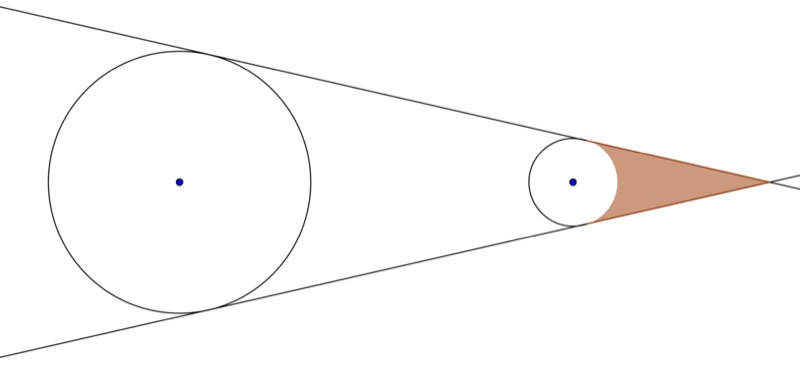
\includegraphics[width=8cm]{ueb59}
%\end{center}

\item Wahr oder falsch?
\begin{enumeratea}
\item W\"urfel sind einander \"ahnlich.
\item Quader sind einander \"ahnlich.
\item Kugeln sind einander \"ahnlich.
\item Zylinder sind einander \"ahnlich.
\end{enumeratea}
\item Ein W\"urfel der Kantenl\"ange $\unit[5]{cm}$ wird mit dem Streckungsfaktor $8$ gestreckt. Welche Kantenl\"ange hat der Bildw\"urfel?

\item Der W\"urfel links wurde von $Z$ aus zentrisch gestreckt.
\begin{center}
\definecolor{qqqqff}{rgb}{0,0,1}
\definecolor{zzzzzz}{rgb}{0.6,0.6,0.6}
\scalebox{0.92}{
\begin{tikzpicture}[line cap=round,line join=round,>=triangle 45,x=0.8cm,y=0.8cm]
\draw [color=zzzzzz,dash pattern=on 2pt off 2pt, xstep=0.475cm,ystep=0.475cm] (-0.73,1.36) grid (15.31,8.78);
\clip(-0.73,1.36) rectangle (15.31,8.78);
\draw (3.5,4)-- (3.5,5);
\draw (3.5,5)-- (4.5,5);
\draw (4.5,5)-- (4.5,4);
\draw (3.5,4)-- (4.5,4);
\draw (3.5,5)-- (3.89,5.36);
\draw (4.5,5)-- (4.88,5.36);
\draw (3.89,5.36)-- (4.88,5.36);
\draw (3.5,4)-- (3.88,4.35);
\draw (4.5,4)-- (4.89,4.35);
\draw (4.88,5.36)-- (4.89,4.35);
\draw (3.89,5.36)-- (3.88,4.35);
\draw (3.88,4.35)-- (4.89,4.35);
\draw (9.5,3)-- (9.5,6);
\draw (9.5,6)-- (12.5,6);
\draw (12.5,6)-- (12.5,3);
\draw (9.5,3)-- (12.5,3);
\draw (9.5,6)-- (10.68,7.08);
\draw (12.5,6)-- (13.63,7.08);
\draw (10.68,7.08)-- (13.63,7.08);
\draw (9.5,3)-- (10.63,4.04);
\draw (9.5,3)-- (10.63,4.04);
\draw (12.5,3)-- (13.68,4.04);
\draw (13.63,7.08)-- (13.68,4.04);
\draw (10.68,7.08)-- (10.63,4.04);
\draw (10.63,4.04)-- (13.68,4.04);
\draw [dotted] (0.5,4.5)-- (3.89,5.36);
\draw [dotted] (3.89,5.36)-- (10.67,7.08);
\fill [color=qqqqff] (0.5,4.5) circle (1.5pt);
\draw[color=qqqqff] (0.35,4.8) node {$Z$};
\end{tikzpicture}
}
\end{center}
\begin{enumeratea}
\item Wie gross ist der Streckungsfaktor?
\item In welchem Verh\"altnis stehen die Kantenl\"angen von Bild- und Originalw\"urfel?
\item In welchem Verh\"altnis stehen die Inhalte der Seitenfl\"achen von Bild- und Originalw\"urfel?
\item In welchem Verh\"altnis stehen die Volumen von Bild- und Originalw\"urfel?
\end{enumeratea}
\item Ein W\"urfel wird zentrisch gestreckt, so dass sich die Kantenl\"angen des Bildw\"urfels zu den Kantenl\"angen des Originalw\"urfels wie $3\div2$ verhalten. Wie verhalten sich
\begin{enumeratea}
\item die L\"angen der K\"orperdiagonalen,
\item die Inhalte der Seitenfl\"achen,
\item die Volumen?
\end{enumeratea}
\item Zwei W\"urfel aus dem gleichen Material wiegen $\unit[1]{kg}$ und $\unit[8]{kg}$. Wie verhalten sich
\begin{enumeratea}
\item ihre Volumen,
\item ihre Kantenl\"angen,
\item die Inhalte ihrer Seitenfl\"achen?
\end{enumeratea}
\item Die Volumen zweier W\"urfel verhalten sich wie $1\div27$. Wie verhalten sich ihre Seitenfl\"acheninhalte?
\item Ein Quader ist $\unit[6]{cm}$ lang, $\unit[4]{cm}$ breit und $\unit[7]{cm}$ hoch. Er wird mit dem Streckungsfaktor $\frac{1}{2}$ zentrisch gestreckt. Welche L\"ange, Breite und H\"ohe hat der Bildquader?
\item

\begin{enumeratea}
\item Die Kantenl\"angen eines Quaders $A$ sind doppelt so lang wie die entsprechenden Kantenl\"angen eines \"ahnlichen Quaders $B$. Wie verhalten sich die entsprechenden Seitenfl\"achen von $A$ und $B$?
\item Die Inhalte der Seitenfl\"achen eines Quaders $C$ sind viermal kleiner als die Inhalte der entsprechenden Seitenfl\"achen eines \"ahnlichen Quaders $D$. Wie verhalten sich entsprechende Kantenl\"angen von $C$  und $D$?
\item Die Kantenl\"angen eines Quaders $E$ sind dreimal kleiner als die entsprechenden Kantenl\"angen eines \"ahnlichen Quadrats $F$. Wie verhalten sich die Volumen von $E$ und $F$?
\item Die Inhalte der Seitenfl\"achen eines Quaders $J$ sind neunmal gr\"osser als die Inhalte der entsprechenden Seitenfl\"achen eines \"ahnlichen Quaders $K$. Wie verhalten sich die entsprechenden Kantenl\"angen von $J$ und $K$?
\item Das Volumen eines Quaders $G$ ist tausendmal gr\"osser als das Volumen eines \"ahnlichen Quaders $H$. Wie verhalten sich die entsprechenden Kantenl\"angen von $G$ und $H$?
\item Das Volumen eines Quaders $L$ ist $64$ mal kleiner als das Volumen eines \"ahnlichen Quaders $M$. Wie verhalten sich die Inhalte entsprechender Seitenfl\"achen von $L$ und $M$?
\end{enumeratea}
\item Die Durchmesser zweier Kugeln verhalten sich wie $4\div5$. Wie verhalten sich ihre Volumen?
\item Die Volumen zweier Kugeln verhalten sich wie $8\div27$. Wie verhalten sich ihre Radien?
\item Zwei Kugeln aus gleichem Material wiegen $\unit[1]{g}$ und $\unit[64]{g}$. Die leichtere Kugel hat einen Durchmesser von $\unit[3]{mm}$. Welchen Durchmesser hat die schwerere Kugel?

\item Eine Kugel wiegt $\unit[16]{kg}$, eine andere aus gleichem Material $\unit[54]{kg}$. Gib in m\"oglichst einfachen ganzen Zahlen an:
\begin{enumeratea}
\item das Verh\"altnis der Volumen,
\item das Verh\"altnis der Durchmesser,
\item das Verh\"altnis der Oberfl\"acheninhalte.
\end{enumeratea}
\item In der Kanalisation einer Siedlung sind die Abflussrohre \"uberlastet. Sie werden durch Rohre mit doppelt so grossem Durchmesser ersetzt. Wie ver\"andert sich das Fassungsverm\"ogen?
\item Die H\"ohe einer quadratischen Pyramide wird durch einen Schnitt parallel zur Grundfl\"ache halbiert. Wie verhalten sich die Volumen
\begin{enumeratea}
\item der Pyramidenspitze und der ganzen Pyramide zueinander,
\item der Pyramidenspitze und des Pyramidenstumpfs zueinander?
\end{enumeratea}
\item In welchem Abstand von der Spitze eines Kegels mit der H\"ohe $h$ muss parallel zur Grundfl\"ache ein Schnitt gelegt werden, wenn das Volumen dadurch im Verh\"altnis $8\div19$ geteilt werden soll?

\item Eine \"agyptische Pyramide mit quadratischem Grundriss wird von waagrecht abgelagertem W\"ustensand allm\"ahlich begraben. Die H\"ohe der noch sichtbaren Pyramide betr\"agt nur noch vier F\"unftel der H\"ohe der urspr\"unglichen Pyramide.
\begin{enumeratea}
\item Wie verhalten sich die Volumen des sichtbaren und des versch\"utteten Teils zueinander?
\item Wie viele $\%$ des urspr\"unglichen Pyramidenvolumens ragen noch aus dem Sand?
\end{enumeratea}

\item Die beiden massiven K\"orper sind zueinander \"ahnlich und aus gleichem Material.
\begin{center}
\begin{tikzpicture}[line cap=round,line join=round,>=triangle 45,x=1.1319100391134291cm,y=1.1319100391134291cm]
\clip(2.54,1.8) rectangle (14.91,7.28);
\draw [line width=1.6pt] (3.5,5)-- (6,5);
\draw [line width=1.6pt] (3.5,5)-- (3.5,4);
\draw [line width=1.6pt] (3.5,4)-- (6,4);
\draw [line width=1.6pt] (6,4)-- (6,5);
\draw [line width=1.6pt] (6,5)-- (6.5,5.5);
\draw [line width=1.6pt] (6,4)-- (6.5,4.5);
\draw [line width=1.6pt] (6.5,4.5)-- (6.5,5.5);
\draw [line width=1.6pt] (5,6)-- (5.5,6);
\draw [line width=1.6pt] (5.5,6)-- (5.75,6.28);
\draw [line width=1.6pt] (5,6)-- (5.28,6.28);
\draw [line width=1.6pt] (5.28,6.28)-- (5.75,6.28);
\draw [line width=1.6pt] (3.5,5)-- (4,5.5);
\draw [line width=1.6pt] (5,6)-- (3.5,5);
\draw [line width=1.6pt] (5.5,6)-- (6,5);
\draw [line width=1.6pt] (5.75,6.28)-- (6.5,5.5);
\draw [line width=1.6pt] (4,5.5)-- (5.28,6.28);
\draw [line width=1.6pt] (9,3)-- (12.76,3.01);
\draw [line width=1.6pt] (9,3)-- (9,4.5);
\draw [line width=1.6pt] (12.76,3.01)-- (12.76,4.51);
\draw [line width=1.6pt] (12.76,4.51)-- (9,4.5);
\draw [line width=1.6pt] (12.76,3.01)-- (13.49,3.77);
\draw [line width=1.6pt] (12.76,4.51)-- (13.49,5.25);
\draw [line width=1.6pt] (13.49,3.77)-- (13.49,5.25);
\draw [line width=1.6pt] (9,4.5)-- (9.75,5.25);
\draw [line width=1.6pt] (11.5,6)-- (12.25,6.01);
\draw [line width=1.6pt] (12.25,6.01)-- (12.68,6.43);
\draw [line width=1.6pt] (11.5,6)-- (11.99,6.43);
\draw [line width=1.6pt] (11.99,6.43)-- (12.68,6.43);
\draw [line width=1.6pt] (9,4.5)-- (11.5,6);
\draw [line width=1.6pt] (12.76,4.51)-- (12.25,6.01);
\draw [line width=1.6pt] (12.68,6.43)-- (13.49,5.25);
\draw [line width=1.6pt] (9.75,5.25)-- (11.99,6.43);
\draw (5.2,6.8) node[anchor=north west] {4.8};
\draw (2.9,5.51) node[anchor=north west] {8.4};
\draw (4.39,3.89) node[anchor=north west] {13.2};
\draw (6.5,5.2) node[anchor=north west] {7.2};
\draw (8.6,5.2) node[anchor=north] {12.6};
\draw (12.1,6.9) node[anchor=north west] {7.2};
\draw (13.57,4.57) node[anchor=north west] {10.8};
\draw (10.59,2.91) node[anchor=north west] {19.6};
\end{tikzpicture}
\end{center}
\begin{enumeratea}
\item Beim gr\"osseren K\"orper steht eine falsche Zahl. Korrigiere sie.
\item Wie viel wiegt der kleinere K\"orper, wenn der gr\"ossere $\unit[16.2]{kg}$ wiegt?
\end{enumeratea}
\end{enumerate}

%\vspace*{-7ex}

\subsection{Testlauf}
\begin{enumerate}
\item Zeichne bei der abgebildeten Figur alle Symmetrieachsen ein.
\begin{center}
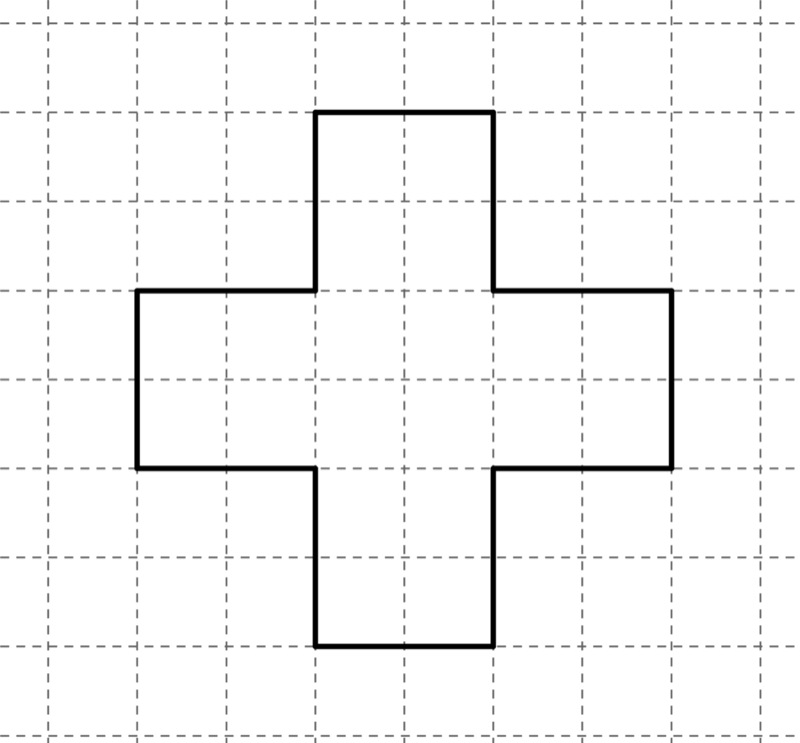
\includegraphics[width=5cm]{pictures/seueb1}
\end{center}
\item Strecke das abgebildete Dreieck vom Punkt $Z$ aus mit dem Streckungsfaktor $2$.
\begin{center}
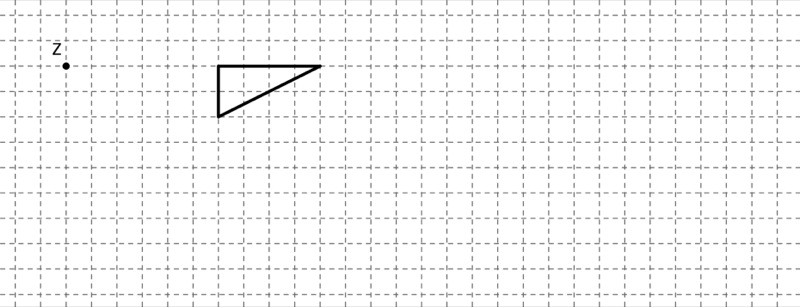
\includegraphics[width=12cm]{pictures/seueb2}
\end{center}
\item Drehe die abgebildete Figur um den Punkt $Z$ um $90^\circ$.
\begin{center}
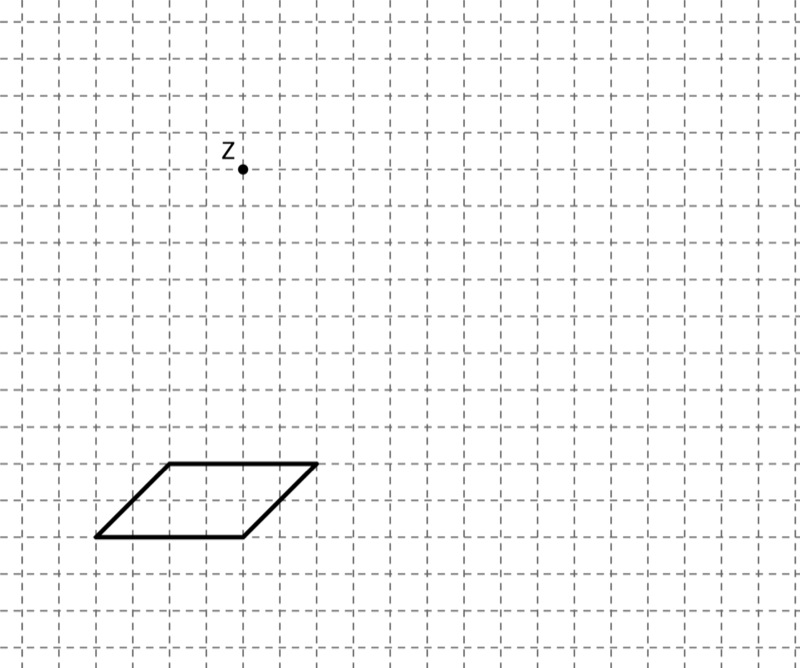
\includegraphics[width=8cm]{pictures/seueb3}
\end{center}

\item Ein gegebenes Dreieck soll von einem gegebenen Punkt aus zentrisch gestreckt werden. Welchen Streckungsfaktor muss man w\"ahlen, um den Umfang des Dreiecks zu vervierfachen?
\item Berechnen Sie die H\"ohe eines Mastes, dessen Schatten eine L\"ange von $\unit[55]{m}$ hat, wenn gleichzeitig der Schatten eines $\unit[180]{cm}$ grossen Mannes $\unit[4.5]{m}$ lang ist.
\item Berechne $x$
\begin{center}
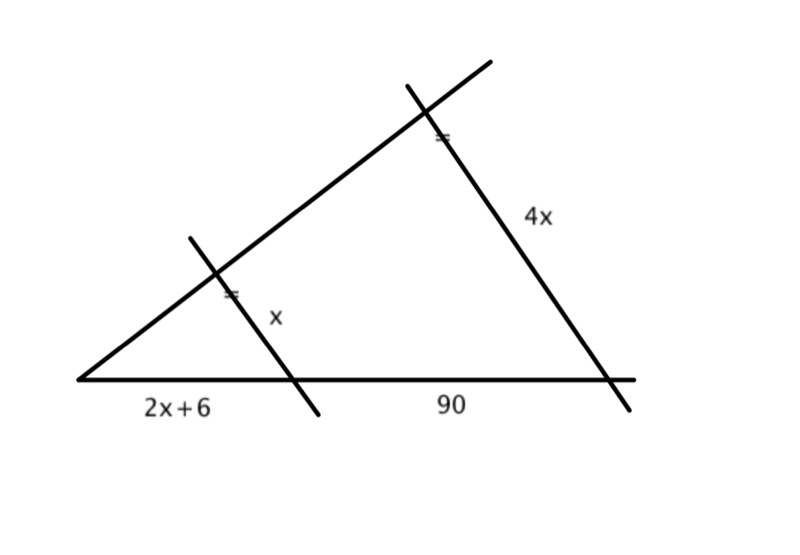
\includegraphics[width=12cm]{pictures/seueb6}
\end{center}
\item Die Durchmesser zweier kugelf\"ormiger Planeten verhalten sich wie $1\div9$. In welchem Verh\"altnis stehen ihre Oberfl\"achen zueinander?
\item Auf einer Karte im Massstab $1\div25\,000$ wird eine Seeoberfl\"ache zu $\unit[416]{cm^2}$ bestimmt. Wie viele Quadratkilometer misst die Seeoberfl\"ache in Wirklichkeit?
\item Ein gerader Kreiskegel wird durch zwei Schnitte parallel zur Grundfl\"ache in drei gleich hohe St\"ucke geteilt. Wie verh\"alt sich das Volumen des obersten zum Volumen des untersten St\"ucks?

\end{enumerate}

\cleardoublepage

\appendix

%\onecolumn

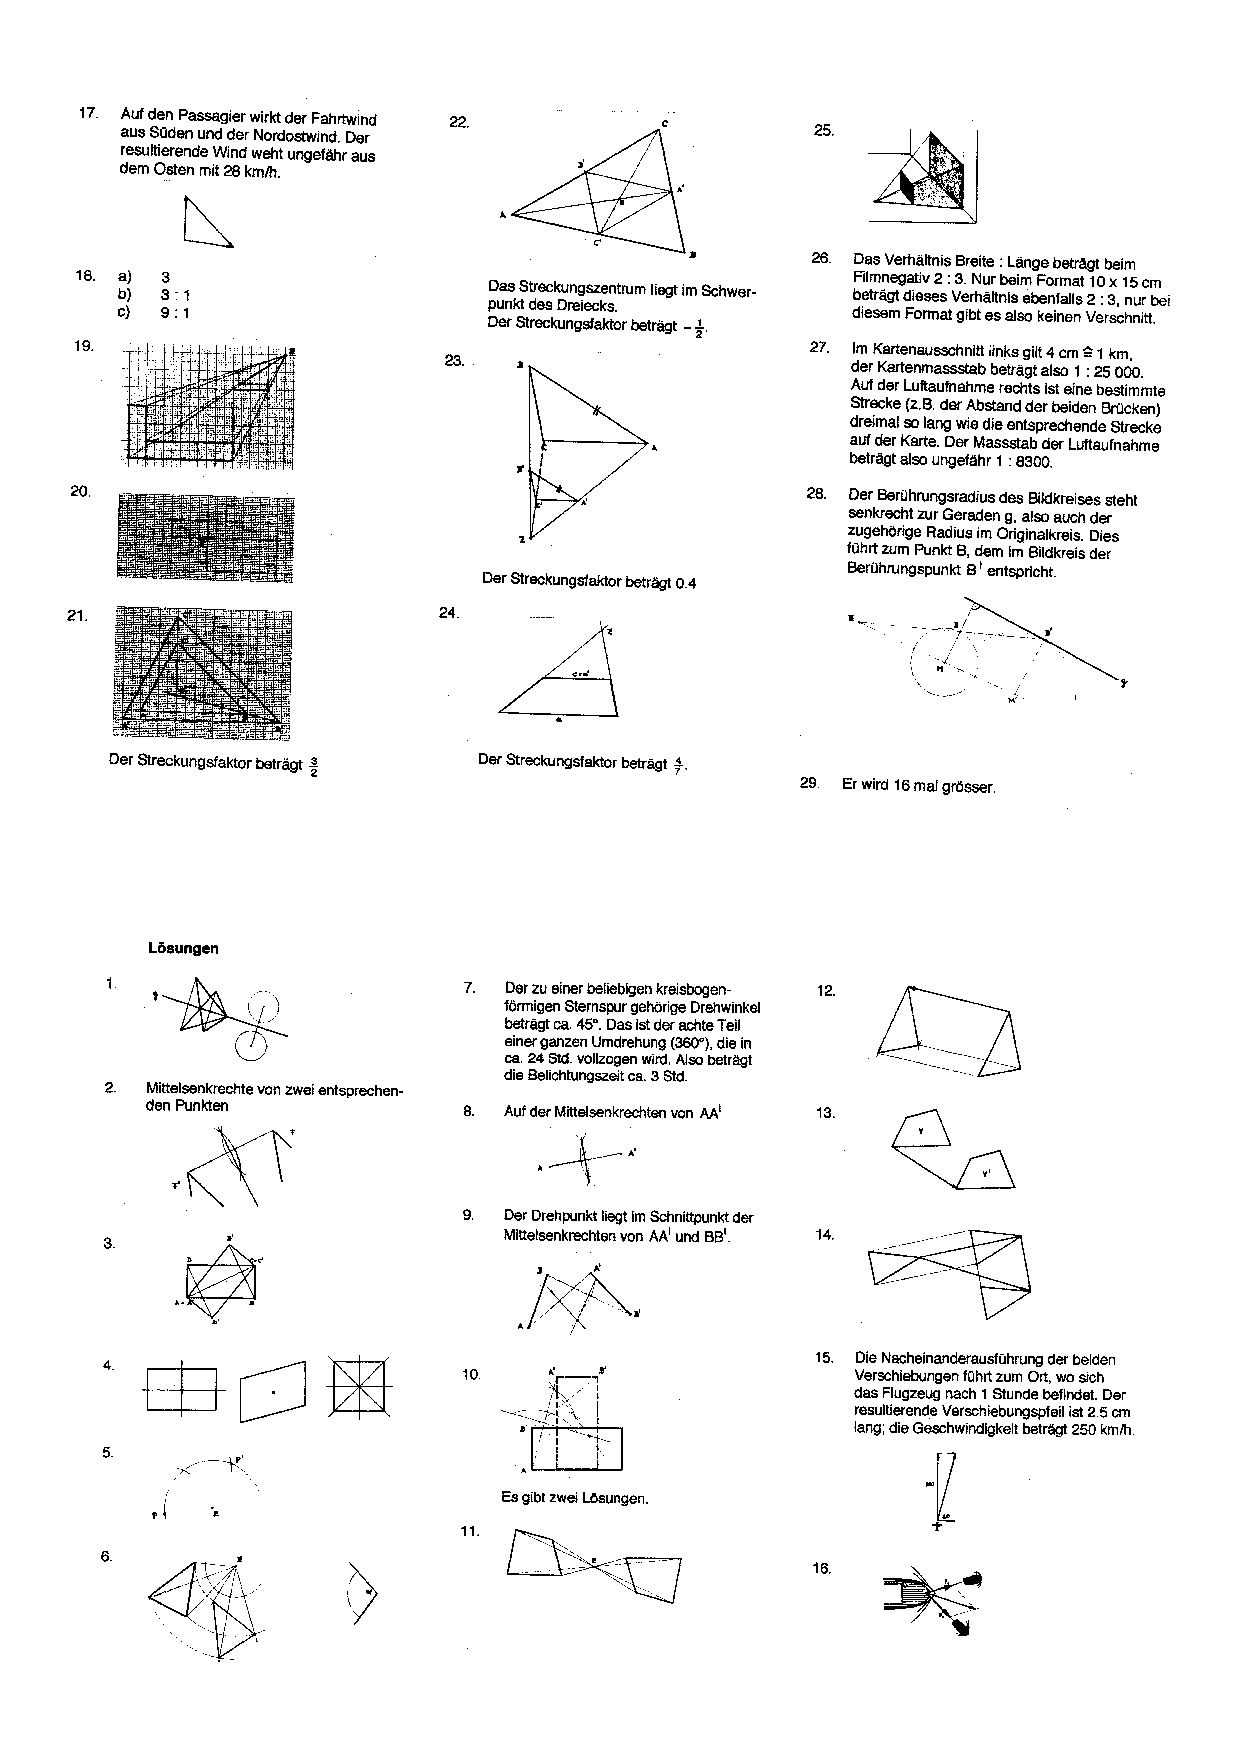
\includepdf[pages={1},scale=0.75,pagecommand=\section{Lösungen zur Ähnlichkeit}]{pictures/aehnlichkeitlsg2}

\includepdf[pages={2},scale=0.75,pagecommand={}]{pictures/aehnlichkeitlsg2}

\clearpage

\section{Satz von Pythagoras}

Wer kennt ihn nicht\dots 

\begin{csatz}[Satz von Pythagoras]{}
Sind $a$, $b$ und $c$ die Seitenlängen eines rechtwinkligen Dreiecks, wobei $a$ und $b$ die Längen der Katheten sind und $c$ die Länge der Hypotenuse ist, so gilt 
$$a^2+b^2=c^2.$$
Die Umkehrung gilt auch!
\end{csatz}

Aber hast du bereits einmal einen Beweis gesehen? Auf der Website \url{http://www.cut-the-knot.org/pythagoras/index.shtml} sind in englischer Sprache $68$ von \"uber $300$ Beweisen aufgef\"uhrt.

\clearpage

\section{Projektive Geometrie}
Im sp\"aten 13. Jahrhundert entstanden in Italien die Stadtrepubliken Florenz, Venedig, Mailand und Genua. Sie erlangten politische und wirtschaftliche Bedeutung und hatten dadurch entscheidenden Anteil daran, dass sich ein neues Menschenbild durchsetzen konnte. Die christlichen Schriftsteller des Mittelalters hatten die Bedeutung des menschlichen Lebens in der Vorbereitung auf das Jenseitige gesehen und gelehrt, dass sich der Mensch m\"oglichst vom Diesseitigen abwenden sollte. Intensive Studien der Schriften der griechischen und r\"omischen Antike, also eine Wiederentdeckung der Antike (Renaissance =Wiedergeburt), f\"uhrten aber dann zu einer neuen Auffassung, die dem einzelnen Menschen Verantwortung \"ubergab und ihn in den Mittelpunkt der Welt stellte. Auch die Kunst, die durch die erstarkten Stadtrepubliken besonders gef\"ordert wurde, wandte sich dem Diesseitigen zu und r\"uckte den Menschen und seine nat\"urliche Umgebung in den Mittelpunkt des k\"unstlerischen Schaffens. Dabei musste ein zentrales geometrisches Problem gel\"ost werden:

\begin{quote}
Wie kann man die dreidimensionale reale Welt auf einer zweidimensionalen Leinwand darstellen?
\end{quote}

\begin{figure}[h!]
\begin{center}
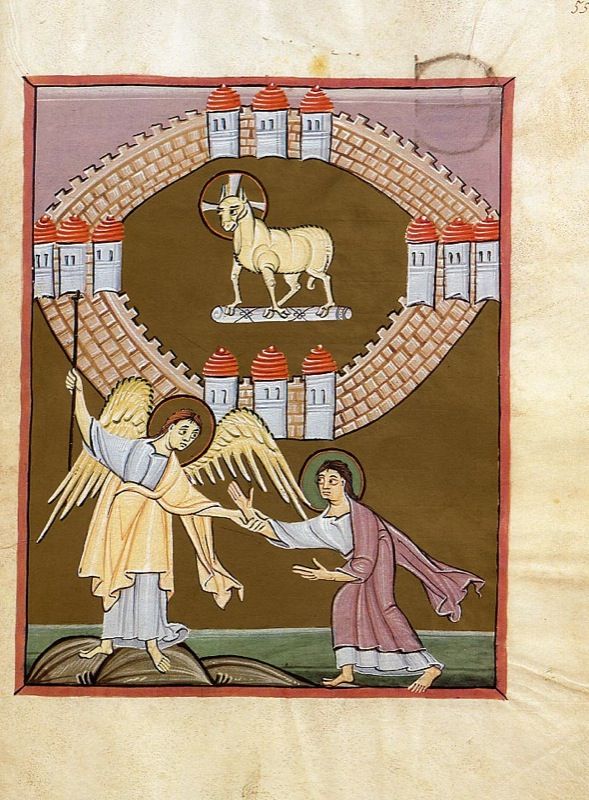
\includegraphics[width=0.54\textwidth]{pictures/tafel39}
\caption{Johannes Apokalypse, Tafel 39, Bramberger Buchmalerei}
\end{center}
\end{figure}

Gesucht wurde eine Methode, die einem Bild den Anschein der Dreidimensionalit\"at verleiht, also ein realistisches Abbild schafft. Die L\"osung fand man in der Entdeckung der Zentralperspektive bzw. perspektivischen Darstellung. Dadurch erhielten die Bilder eine grosse r\"aumliche Tiefe und nat\"urliche Echtheit.

Die mittelalterlichen Malereien waren \glqq konzeptional\grqq, der wichtigste Gegenstand wurde bevorzugt behandelt, selbst wenn dadurch das Bild verzerrt wurde. Typisch f\"ur diesen nicht perspektivischen Malstil ist die Illumination aus dem 12. Jahrhundert eines unbekannten Malers. Die Burg verschwindet fast vor den Schiffen angreifender Krieger, die Schiffe oben im Bild, die sich in weiter Entfernung am Horizont befinden, sind genau so gross wie die Schiffe im Vordergrund.

Die K\"unstler der Renaissance waren meist zugleich Maler, Goldschmiede, Architekten, Ingenieure und Festungsbaumeister. Sie entwarfen und bauten Kirchen, Hospit\"aler, Pal\"aste, Kl\"oster, Br\"ucken, D\"amme, Kan\"ale, Waffen etc. Da sie perspektivische Darstellungen dringend f\"ur die Aus\"ubung ihres Berufes brauchten, fanden diese Artefici notgedrungen L\"osungen f\"ur die Grundprobleme der darstellenden Geometrie. So wurden die K\"unstler des 15. Jahrhunderts auch zu bedeutenden Mathematikern ihrer Zeit.

\textsc{Giottodi Bondone} (1266-1337), \textsc{Van Eyck} (1390-1441), \textsc{Brunelleschi} (1377-1446), \textsc{Alberti} (1404-1472) hatten bereits erste, f\"ur die Zukunft tragbare Erfolge bei der Meisterung des Problems der Perspektive erzielt.

Der Florentiner \textsc{Filippo Brunelleschi}, der ber\"uhmte Baumeister der Domkuppel, beispielsweise wollte \"offentlich beweisen, dass Fl\"achenkunst die Vollkommenheit angewandter Mathematik erreichen kann. Um dies zu beweisen, hatte er unter anderem eine Tafel gemalt, f\"ur die man einen Standort nahe dem Hauptportal und in der Mittelachse des Domes zu w\"ahlen hatte.

Alles, was man von dieser Stelle aus, durch das ge\"offnete Portal hindurch vom Baptisterium und dessen Nachbarbauten sehen konnte, hatte er auf der Tafel mit Farben festgehalten. Die Tafel war in der Mitte vorsichtig gelocht und wurde dem Interessenten zusammen mit einem Spiegel ausgeh\"andigt.

Mit der einen Hand fasste man den Spiegel, mit der anderen die Tafel. Wenn man deren unbemalte R\"uckseite so vors Auge hielt, dass man durch das kleine Loch blicken konnte, und sich gleichzeitig mittels des vor die Vorderseite gehaltenen Spiegels das Gemalte widerspiegeln liess, erhielt man den Eindruck, genau diejenige Wirklichkeit vor
sich zu sehen, die man, wenn der
Spiegel weggenommen wurde, real vor sich sah. Der T\"auschungseffekt war um so erstaunlicher, als er sich sogar auf Bewegliches bezog. Brunelleschi hatte n\"amlich den Himmelsbezirk auf seiner Tafel mit Silberfolie belegt, so dass im Spiegelbild mit der Starrheit der Architektur der Wandel der Wolken kontrastierte. Das Abbild erschien, \"uber alle lineare und farbige †bereinstimmung hinaus, auch noch lebendig.

Die Ideen Brunelleschis wurden von \textsc{Alberti} weiterentwickelt; er schreibt den ersten allgemeinen Traktat \"uber die Perspektive. Zur vollen Meisterschaft in der Kunst der Perspektive brachten es aber erst sp\"ater \textsc{Leonardo da Vinci} (1452- 1519) in Italien und \textsc{Albrecht D\"urer} (1471-1528) in Deutschland.

Der Schl\"ussel zur dreidimensionalen Darstellung liegt in dem Prinzip 'Projektion und Schnitt': Der Maler stellt sich vor, dass von jedem Punkt der zu malenden Szene aus ein Lichtstrahl in sein Auge f\"allt (Zentralprojektion). Zwischen die zu malende Szene und seinem Auge wird
eine Glasscheibe, die seiner Leinwand entspricht, aufgestellt. Auf dieser Glasscheibe werden nun Punkt f\"ur Punkt die Stellen markiert, in denen die Projektions- oder Sehstrahlen die Scheibe durchdringen (Durchstosspunkte). Die Menge aller derartigen Punkte ist ein \glqq Schnitt\grqq. Die Renaissance-K\"unstler hatten entdeckt, dass bei der Betrachtung eines \glqq Schnittes\grqq\ derselbe Eindruck entsteht, als wenn man die Szene direkt anschaut. Denn das Licht, das von einem Objektpunkt ausgeht und in unser Auge f\"allt, verl\"auft geradlinig; die Lichtstrahlen, die von den entsprechenden Punkten auf der Glasscheibe ausgehen, verlaufen auf denselben Geraden. Deshalb muss derselbe Eindruck entstehen. Der Maler hatte jetzt nur noch den \glqq Schnitt\grqq, der auf der Glasscheibe erscheint, auf die Leinwand, die nicht durchsichtig und zweidimensional ist, zu \"ubertragen, um ein realistisches Bild zu erzielen. \textsc{D\"urer} benutzte f\"ur dieses Prinzip das Wort \emph{Perspektive} (perspicere, lat.: hindurchsehen) und illustrierte dies sehr sch\"on auf mehreren Holzschnitten, die aus seinem Lehrbuch \glqq Underweysung der messung mit dem zirkel und richtscheyed \dots\grqq\ (1525) stammen.

\begin{figure}[h!]
\begin{center}
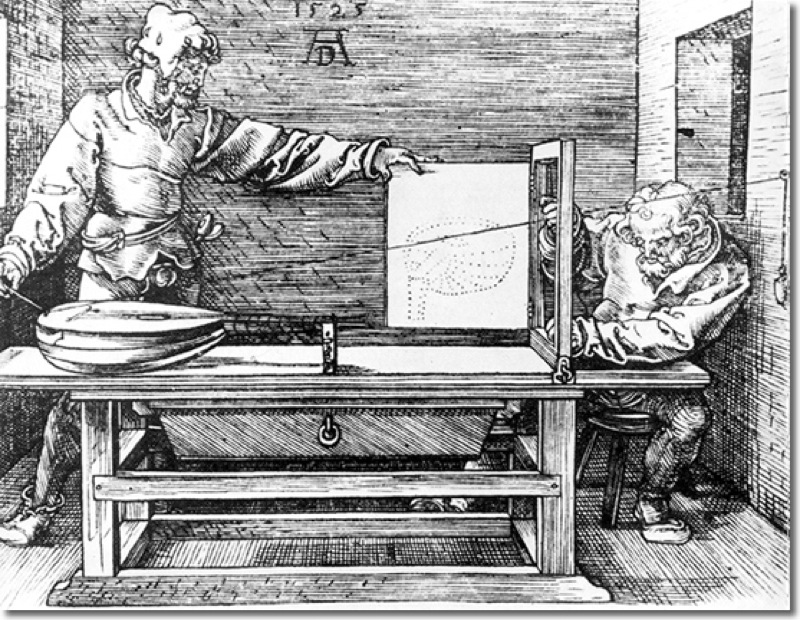
\includegraphics[width=0.618\textwidth]{pictures/durer}
\caption{Aus Albert D\"urers: Underweysung der messun mit dem zirkel und richtscheyed... (1525)}
\end{center}
\end{figure}

Da die Abbildung vom Standpunkt des K\"unstlers und der Placierung der Glasscheibe abh\"angt, gibt es verschiedene Darstellungen von der gleichen Szene. Die dargestellten Objekte k\"onnen verschiedene Gr\"osse haben; ein Bild kann die Szene aus frontaler Sicht zeigen, ein anderes Bild kann dieselbe Szene mehr von der Seite her zeigen. Der Photoapparat ist \"ubrigens ein hervorragendes Beispiel, um das Prinzip "Projektion und Schnitt" zu demonstrieren: Unser Auge, das Projektionszentrum, entspricht der Linse, der 'Schnitt' erscheint auf dem Film. Aus verschiedenen Stellungen erh\"alt man leicht vom gleichen Objekt verschiedene Bilder.

Nach der Wahl des Standpunktes und der Position der Glasscheibe gilt es nun, das Bild auf die Leinwand zu \"ubertragen. Da aber meist die zu malende Szene nur in des K\"unstlers Vorstellung existiert und die Leinwand nicht durchsichtig ist, braucht der K\"unstler Regeln, die stehen durch die Winkel, die die Linien mit der Bildebene bilden. Auf dem Bild von \textsc{Raffael} findet man unter anderem \textsc{Aristoteles, Plato} (mit den Z\"ugen Leonardos), \textsc{Euklid, Epikur, Pythagoras, Empedokles, Heraklit, Diogenes}.

Die erw\"ahnten Grunds\"atze beschreiben nur die einfachsten Dinge, die man wissen muss, um realistisch zu malen. Wie aber erscheinen Kurven auf der Glasscheibe (Leinwand)?
Zum Beispiel zeigt das Bild von \textsc{Lorenzo di Pietro}, dass ein Kreis im allgemeinen nicht als Kreis gemalt werden kann. Er erscheint als Ellipse oder als Parabel- oder Hyperbelbogen auf dem Bild. Dies h\"angt eben davon ab, wo der Kreis sich relativ zum Beobachter befindet. (Stichwort: Kegelschnitte)
Man erkennt, dass realistisches Malen angewandte Mathematik ist. Beim Betrachten eines so konzipierten Bildes sollte man deshalb unbedingt die Position einnehmen, die der Maler bei der Planung des Bildes verwendet hat. Die Bilder der Renaissance-K\"unstler sind meist in Kunstmuseen zu finden, sie k\"onnten genau so gut in naturwissenschaftlichen Museen h\"angen. Liebhaber der Kunst der Renaissance sind bewusst oder unbewusst auch Liebhaber der Naturwissenschaften und der Mathematik!

\begin{figure}[h!]
\begin{center}
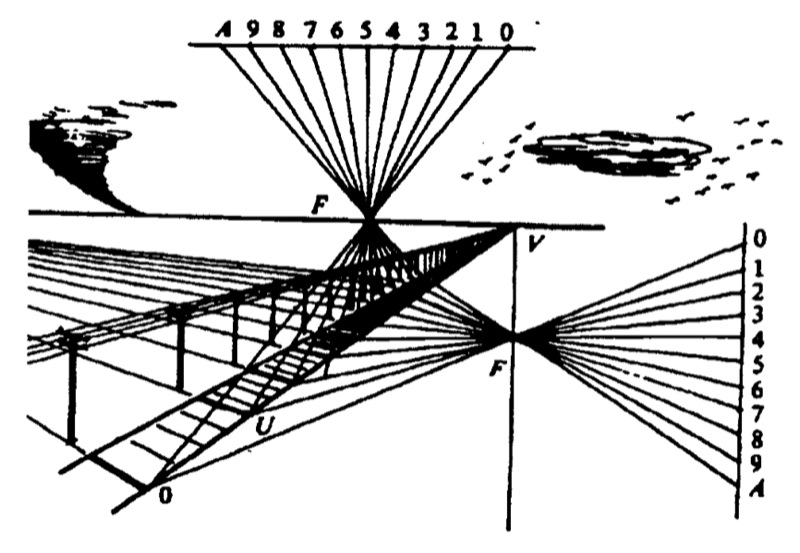
\includegraphics[width=0.618\textwidth]{pictures/eisenbahn}
\end{center}
\caption{Eisenbahn}\label{eisenbahn}
\end{figure}

Abbildung \ref{eisenbahn} zeigt ein konkretes Beispiel, n\"amlich, wie man Eisenbahnschienen mit Schwellen zeichnet, die in eine Landschaft eingebettet sind. Wie sind die Schienen oder die Telegraphenmasten zu positionieren, wo sollen sie im Horizont verschwinden? Man w\"ahlt einen Brennpunkt $F$ verschieden vom Hauptpunkt $V$ und zeichnet die Gerade $FV$. Die Figur zeigt zwei m\"ogliche Wahlen; in dem einen Fall f\"allt $FV$ mit dem Horizont zusammen, im anderen Fall ist $FV$ senkrecht zum Horizont.

Nun nimmt man einen Anfangspunkt $0$ und einen Punkt $U$ auf den Schienen so, dass $OU$ eine Einheitsstrecke wird, an der alle anderen Strecken entlang der Schienen gemessen werden. Als n\"achstes zeichnet man eine Parallele $g$ zu $FV$ und projiziert die Punkte $0$ und $U$ durch $F$ auf $g$. Die Gerade $g$ dient jetzt als perspektivischer Massstab, um die Schwellenabst\"ande entlang der Schienen abzumessen. Eine Folge von \"aquidistanten Punkten auf $g$, zur\"uckprojiziert durch den Brennpunkt $F$ ergibt eine korrekte Perspektive f\"ur die Punkte mit gleichen Abst\"anden auf den Eisenbahnschienen.
Betrachtet man die in der Realit\"at vorhandenen Rechtecke, die aus den beiden Schienen und je zwei Schwellen gebildet werden, so erkennt man:

Das Bild ist weder kongruent, noch \"ahnlich, noch fl\"achengleich zu der Originalfigur.
Die Perspektive ist nicht winkeltreu.

Die Bilder seit der Renaissance zeigen, dass man die geometrische Struktur des Originals auf der Leinwand gut erkennen kann. Dies liegt darin begr\"undet, dass es geometrische Eigenschaften gibt, die invariant gegen\"uber Projektionen sind, also Eigenschaften, die im Bild unver\"andert erscheinen und daher ihre Identifizierung erm\"oglichen. Diese Eigenschaften aufzuzeigen und zu untersuchen ist die Aufgabe der projektiven Geometrie. Eine der fr\"uhesten Entdeckungen der projektiven Geometrie ist der ber\"uhmte Dreieckssatz des franz\"osischen Architekten und Ingenieurs \textsc{Gerard Desargues} (1593-1662). Dieser Satz zeigt die signifikante Eigenschaft, die zwei Schnitten derselben Projektion eines Dreiecks zukommt.

Wenn zwei Dreiecke $ABC$ und $A'B'C'$ in zwei verschiedenen, aber nicht parallelen Ebenen so gelegen sind, dass die Verbindungslinien einander entsprechender Punkte in einem Punkt $0$ kongruent sind (die Dreiecke befinden sich in perspektiver Lage), dann schneiden sich die Verl\"angerungen entsprechender Seiten in drei kollinearen Punkten $R$, $S$ und $T$.

Der Satz von \textsc{Desargues} ist auch richtig, wenn die beiden Dreiecke in einer Ebene liegen.

Die Bilder seit der Renaissance zeigen, dass man die geometrische Struktur des Originals auf der Leinwand gut erkennen kann. Dies liegt darin begr\"undet, dass es geometrische Eigenschaften gibt, die invariant gegen\"uber Projektionen sind. Diese Eigenschaften aufzuzeigen und zu untersuchen ist Aufgabe der projektiven Geometrie.

\begin{ueb}
Wie lautet der Dreieckssatz von \textsc{Gerard Desargues}? Skizzieren Sie die Situation.
\end{ueb}

\begin{figure}[h!]
\begin{center}
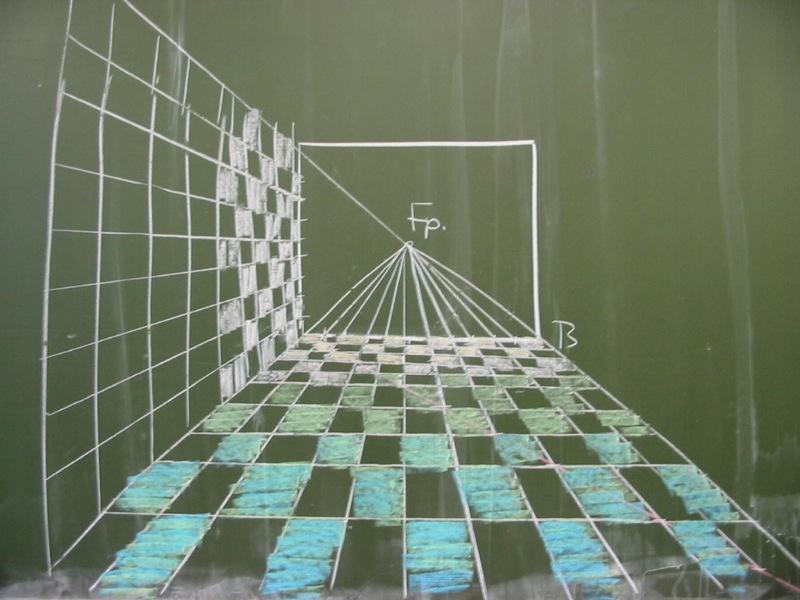
\includegraphics[width=0.8\textwidth]{pictures/fluchtp}
\caption{Wandtafelskizze zur Konstruktion des Fluchtpunktes}
\end{center}
\end{figure}

Viele K\"unstler machen sich die Theorien der Perspektive zu nutze oder spielen damit. Hier noch einige Beispiele:

\begin{figure}[h!]
\begin{center}
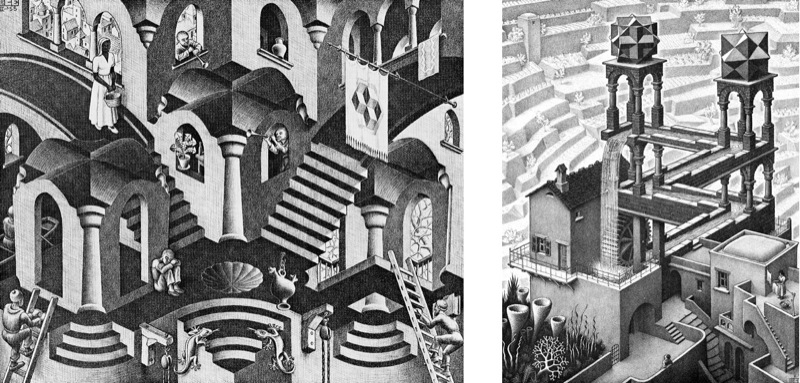
\includegraphics[width=0.618\textwidth]{pictures/escher}
\caption{Bilder von \textsc{Escher}}
\end{center}
\end{figure}

\begin{figure}[h!]
\begin{center}
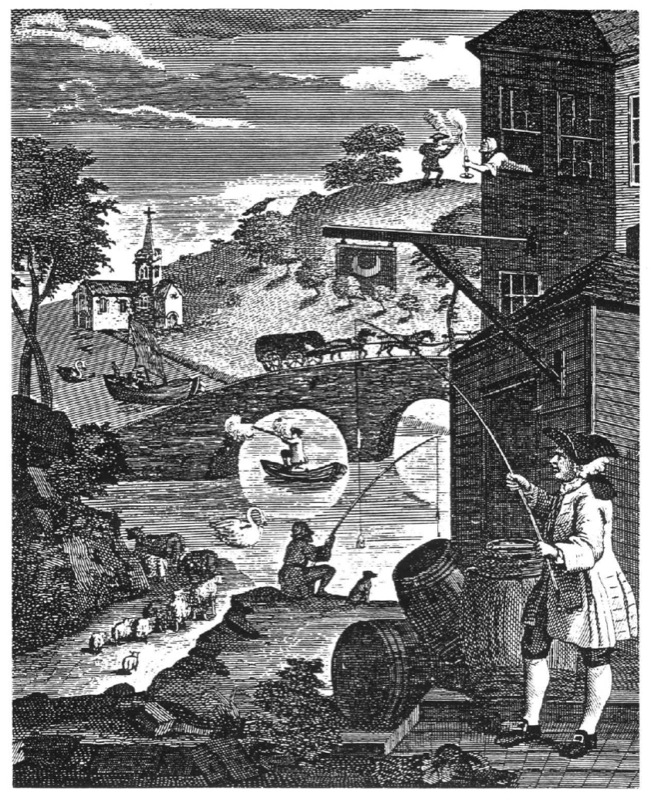
\includegraphics[width=0.618\textwidth]{pictures/hogarth}
\caption{Bild von \textsc{William Hogarth} (1697--1764)}
\end{center}
\end{figure}

\clearpage

\section{Polyeder}
Als Polyeder (griech., Vielfl\"achner) bezeichnet man K\"orper, die nur von ebenen Vielecken begrenzt werden. Beispiele sind W\"urfel, Pyramiden, Prismen; ein Zylinder ist kein Polyeder.

\subsection{Die 5 Platon'schen Polyeder}
Besteht eine Oberfl\"ache eines konvexen Polyeders aus lauter kongruenten Vielecken und treffen in dessen Ecken immer die gleiche Anzahl Fl\"achen zusammen, so spricht man von \emph{regelm\"assigen Polyedern}. Ihre Anzahl ist beschr\"ankt und kann ermittelt werden, wenn man bedenkt:
\begin{itemize}
\item Die Summe aller Kantenwinkel an jeder K\"orperecke muss kleiner als $360^\circ$ sein.
\item In jeder K\"orperecke stossen mindestens $3$ Fl\"achen zusammen.
\end{itemize}
Somit folgt: Wird das Polyeder von regelm\"assigen Dreiecken begrenzt, so kann eine Ecke nur von $3$, $4$ oder $5$ Seitenfl\"achen gebildet werden (Tetraeder, Oktaeder, Ikosaeder). Wird das Polyeder von regelm\"assigen Vierecken (Hexaeder) oder regelm\"assigen F\"unfecken (Dodekaeder) begrenzt, so kann eine Ecke nur durch $3$ Seitenfl\"achen gebildet werden. Andere M\"oglichkeiten gibt es nicht mehr.
\begin{ueb}
Begr\"unden Sie diese Folgerungen.
\end{ueb}
\begin{csatz}[Regulärer Polyedersatz]{}
Es gibt genau $5$ regelm\"assige Polyeder.
\end{csatz}

\begin{figure}[h!]
\begin{center}
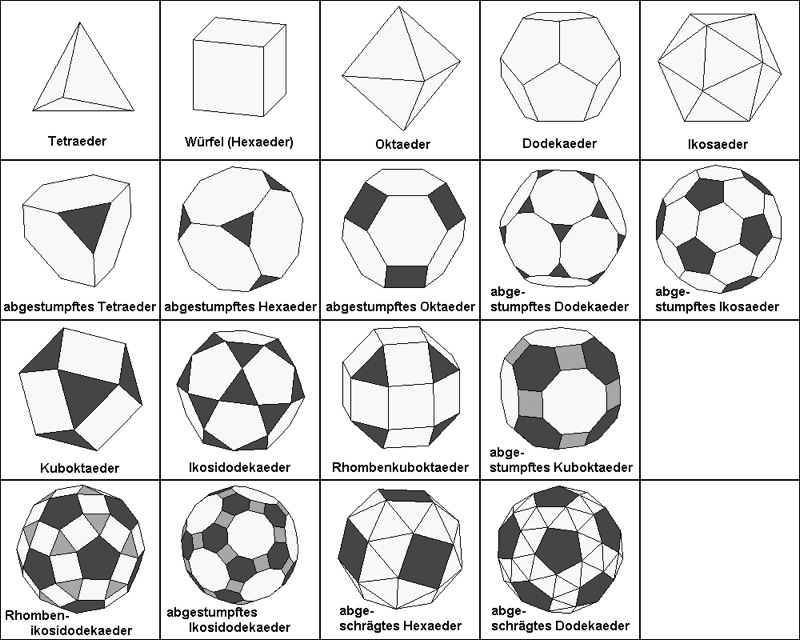
\includegraphics[width=0.8\textwidth]{pictures/polyeders}
\end{center}
\caption{Die f\"unf regelm\"assigen Polyeder mit verwandten}
\end{figure}

F\"ur den griechischen Philosophen \textsc{Plato} (427--347 v.~Chr.) waren diese f\"unf K\"orper Grundbausteine seines Weltsystems: Sie entsprachen den vier Elementen Feuer, Erde, Wasser und Luft. Das Dodekaeder entsprach einer Schale, die das ganze Universum einh\"ullt. Daher werden die f\"unf regelm\"assigen Polyeder auch \emph{platonische K\"orper} genannt.

\begin{figure}[h!]
\begin{center}
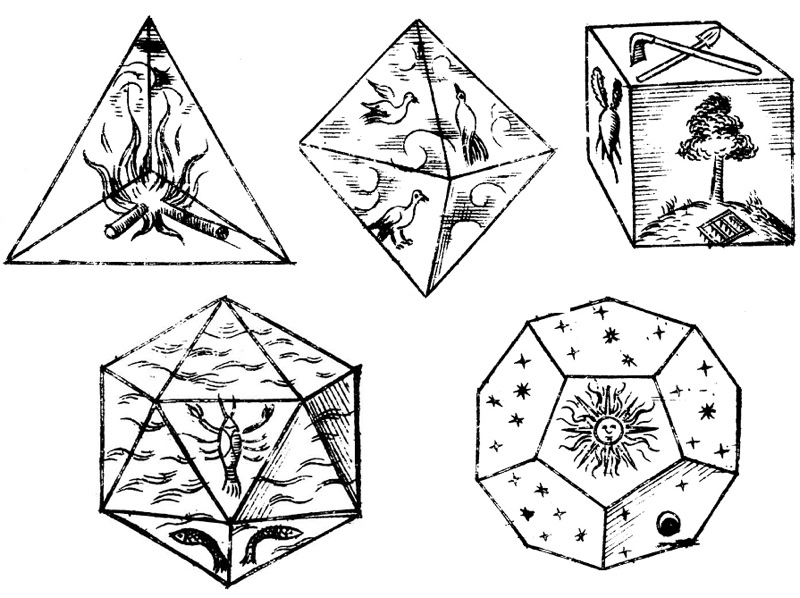
\includegraphics[width=0.382\textwidth]{pictures/platonkoerper}
\end{center}
\caption{Die f\"unf platonischen K\"orper und ihre Bedeutung als Elemente}
\end{figure}

Diese Idee Platons kann als erster bekannter Versuch interpretiert werden, die Welt mit einem Atombild zu erkl\"aren. \textsc{Platon} stellte auch Regeln auf, wie die einzelnen Elemente miteinander reagieren oder ineinander \"ubergef\"uhrt werden k\"onnen.

Die platonischen K\"orper beeindrucken durch ihre vollkommene Gestalt; selbst die Natur bevorzugt beispielsweise bei Kristallformen deren Gestalt.
\begin{figure}
\begin{center}
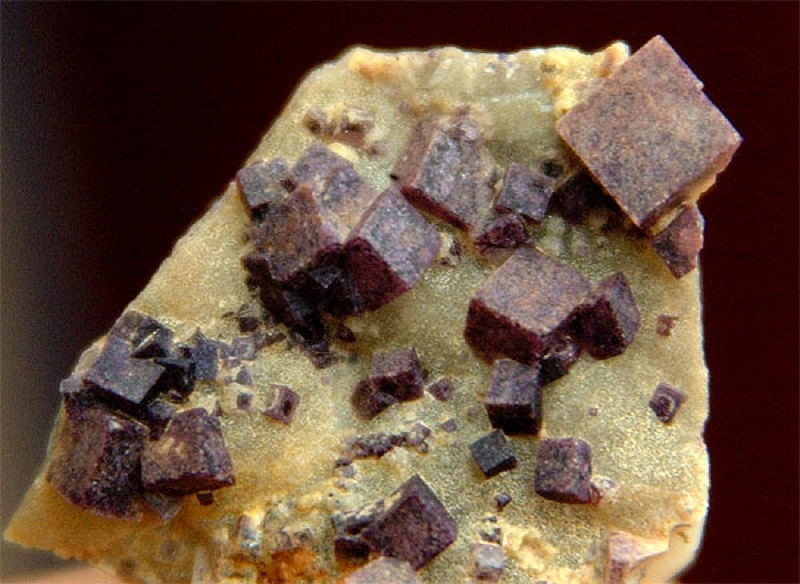
\includegraphics[width=0.382\textwidth]{pictures/kristallh}
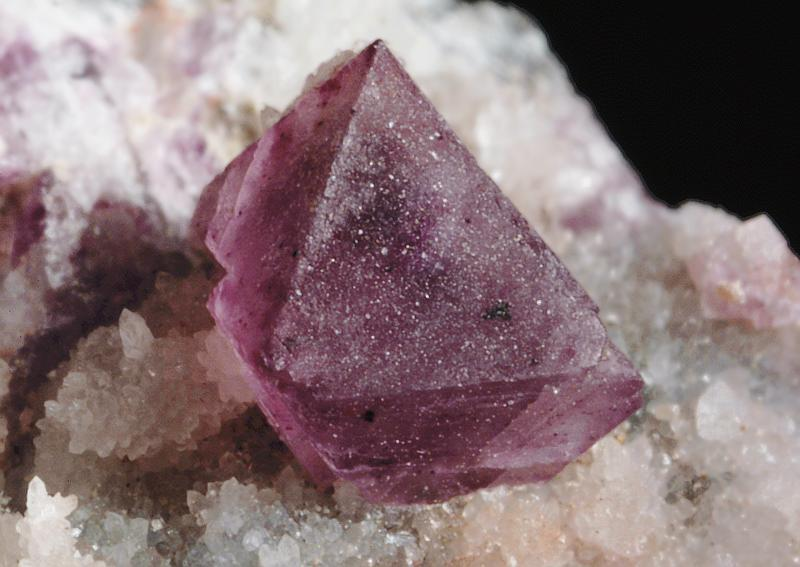
\includegraphics[width=0.382\textwidth]{pictures/kristallo}
\end{center}
\caption{Fluorkristalle (W\"urfel und Oktaeder)}
\end{figure}
Der Astronom \textsc{Johannes Kepler} (1471--1528) benutzte diese regelm\"assigen Polyeder als Modell f\"ur die Bahnen der Planeten.
\begin{figure}
\begin{center}
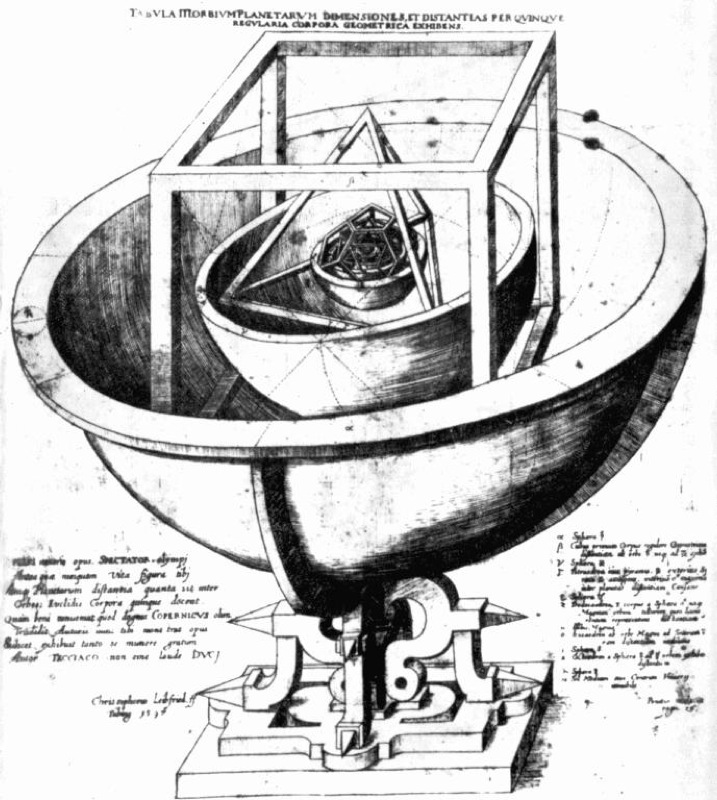
\includegraphics[width=0.618\textwidth]{pictures/kepler}
\end{center}
\caption{Planetenbahnmodell von \textsc{Kepler}}
\end{figure}
Eine der Erdbahn zugeordnete Kugel bildet den Ausgang. Ihr wird ein Dodekaeder umbeschrieben; auf dessen Umkugel liegt die Bahn des Mars. Das dieser Kugel umbeschriebene Tetraeder enth\"alt auf seiner Umkugel die Bahn des Jupiter, und der dieser Kugel umbeschriebene W\"urfel bestimmt eine Umkugel, auf der die Bahn des Saturn verl\"auft. Das der Erdbahnkugel einbeschriebene Ikosaeder tr\"agt auf seiner Inkugel die Bahn der Venus und das dieser Inkugel einbeschrieben Oktaeder enth\"alt auf seiner Inkugel die Bahn des Merkurs.

\begin{ueb}
Welche der Figuren stellen aufgeklappte W\"urfel dar?
\begin{figure}[h!]
\begin{center}
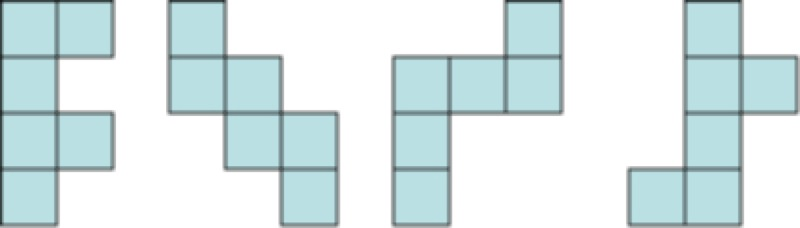
\includegraphics[width=0.382\textwidth]{pictures/wuerfelnetz}
\end{center}
\caption{W\"urfelnetze}
\end{figure}
\end{ueb}

\begin{ueb}
Besorge dir ein mittelstarkes glattes farbiges Zeichenpapier, ein Eisenlineal und ein Messer zum Schneiden und Einritzen. Zeichne die Netze der platonischen K\"orper und bauen Sie sich saubere Modelle.
\end{ueb}

\begin{ueb}
Zeichne zu jedem platonischen K\"orper ein Schr\"agbild. Benutzen Sie beim tetraeder, Oktaeder und Ikosaeder einen W\"urfel, der diesen K\"orper umgibt, beim Dodekaeder einen W\"urfel, der innerhalb des Dodekaeders liegt. Vergleichen Sie mit den Modellen aus der Schulsammlung.
\end{ueb}

\begin{ueb}
F\"ullen Sie folgende Tabelle aus:
\begin{center}
\begin{tabular}{|c|c|c|c|}\hline
\spaltenheight\textbf{K\"orper} & \textbf{Ecken} & \textbf{Fl\"achen} & \textbf{Kanten}\spaltensep \hline
\spaltenheight Tetraeder & & & \spaltensep \hline
\spaltenheight Hexaeder & & & \spaltensep \hline
\spaltenheight Oktaeder & & & \spaltensep \hline
\spaltenheight Dodekaeder & & & \spaltensep \hline
\spaltenheight Ikosaeder & & & \spaltensep \hline
\end{tabular}
\end{center}
Erkl\"are die Namen der platonischen K\"orper. Was f\"allt bei den Zahlen in der Tabelle auf? Bestimme zus\"atzlich alle Symmetrien.
\end{ueb}

\subsection{Der Euler'sche Polyedersatz}
Obwohl sich die griechischen Mathematiker intensiv mit den Polyedern besch\"aftigt haben, wurde der folgende Satz erst von \textsc{Leonard Euler} (1707--1783) entdeckt.
\begin{csatz}[Euler'scher Polyedersatz]
Es sei $E$ die Anzahl Ecken, $K$ die Anzahl Kanten und $F$ die Anzahl Seitenfl\"achen eines beliebigen Polyeders. Dann gilt:
$$E-K+F=2.$$
\end{csatz}
\begin{proof}[Beweis]
Wir haben diesen Satz bereits bei den platonischen K\"orper best\"atigt. Die folgenden Beweisschritte werden am Beispiel eines W\"urfels demonstriert. Man stelle sich dabei vor, dass die Oberfl\"ache des Polyeders aus einer Gummihaut besteht.

\begin{minipage}{0.618\textwidth}
\begin{enumerate}
\item Nach Herausnehmen einer Fl\"ache ($F\rightarrow F-1$) kann man die Oberfl\"ache so stark deformieren, dass sie schliesslich flach in der Ebene liegt.\\
\item Triangulation: In jedem Vieleck, das nicht schon ein Dreieck ist, wird eine Diagonale eingezeichnet: ($K\rightarrow K+1, F\rightarrow F+1$) $E-K+F$ bleibt konstant.\\
\item Bei den Dreiecken, die nur eine Kante auf der Randlinie haben, wird alles entfernt, was nicht zugleich zu anderen Dreiecken geh\"ort: ($K\rightarrow K-1, F\rightarrow  F-1$) $E-K+F$ bleibt konstant.\\
\item Bei den Dreiecken, die zwei Kanten auf der Randlinie haben, wird auch alles entfernt, was nicht zugleich zu anderen Dreiecken geh\"ort: ($E\rightarrow  E-1, K\rightarrow  K-2, F\rightarrow  F-1$) $E-K+F$ bleibt konstant.\\
\item Die Punkte 3. und 4. werden so lange wiederholt, bis zuletzt nur noch ein Dreieck mit $E-K+F=1$ \"ubrig bleibt.\\
\end{enumerate}
\end{minipage}
\hspace*{2cm}
\begin{minipage}{1.7cm}
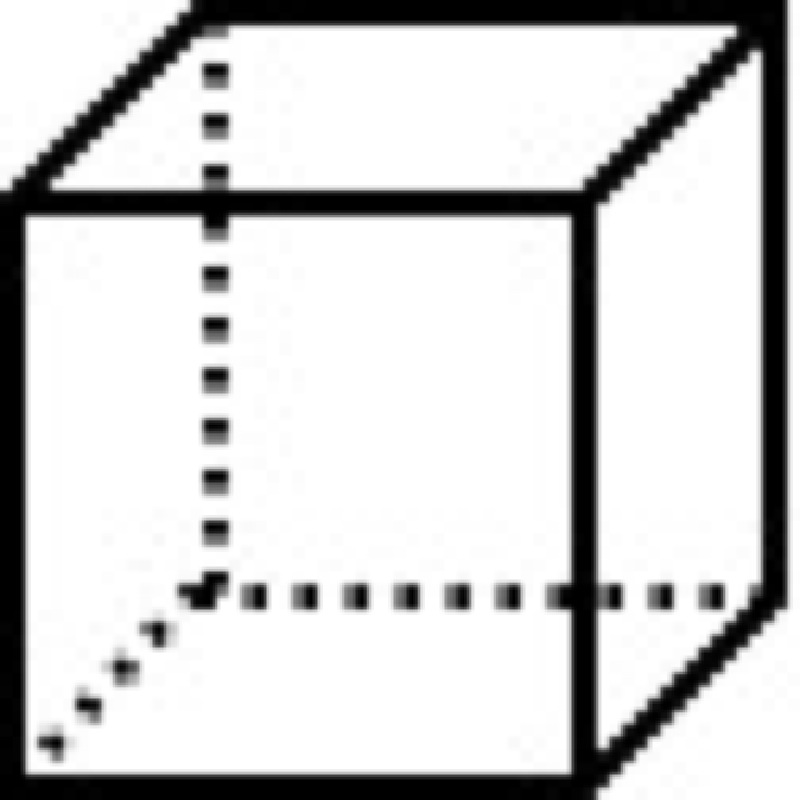
\includegraphics[width=1.7cm]{pictures/wuerf1}\\[3ex]
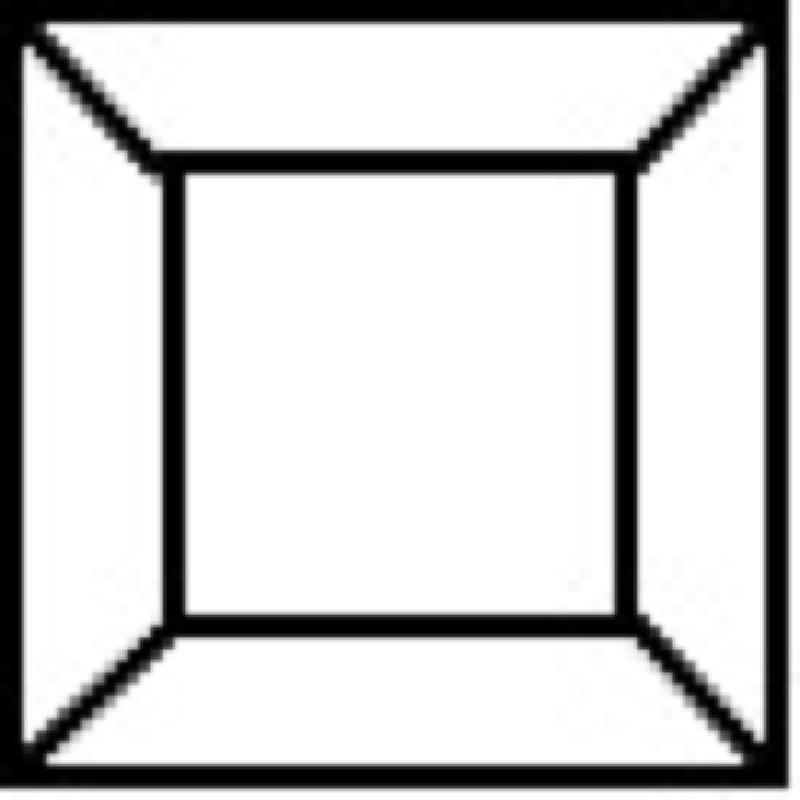
\includegraphics[width=1.7cm]{pictures/wuerf2}\\[4ex]
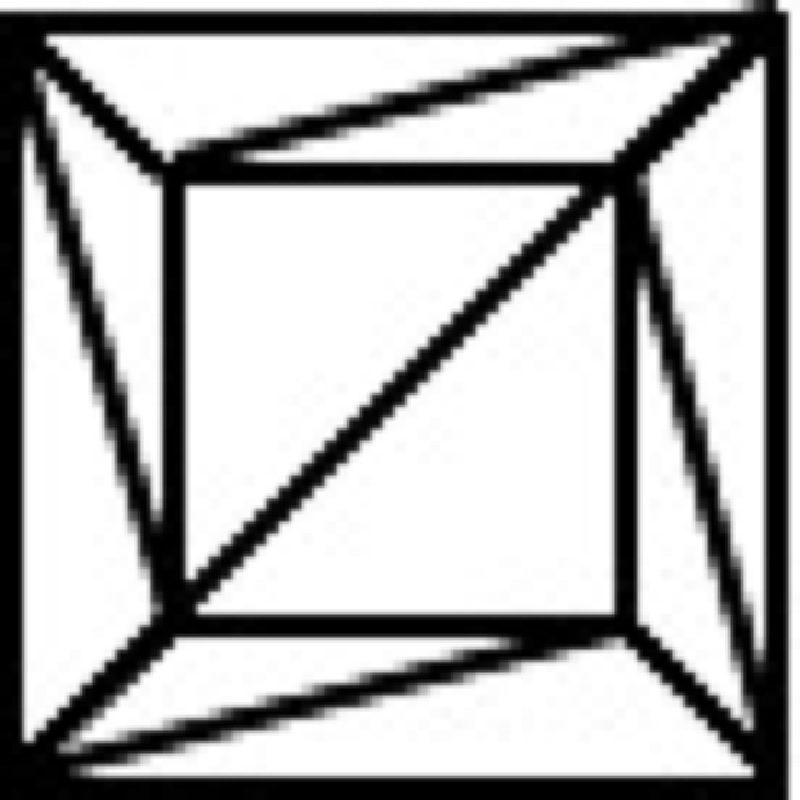
\includegraphics[width=1.7cm]{pictures/wuerf3}\\[5ex]
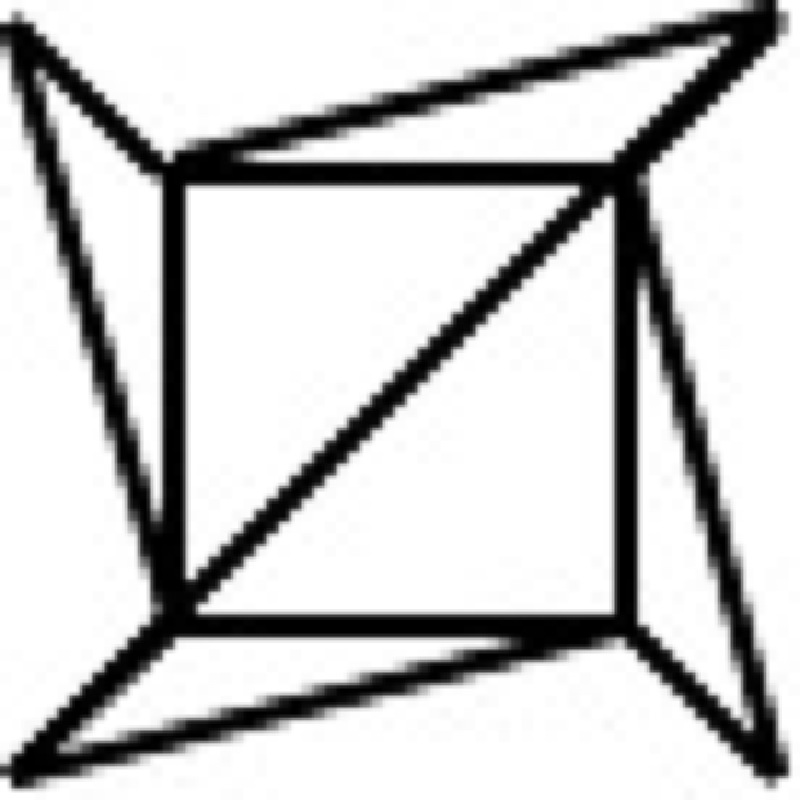
\includegraphics[width=1.7cm]{pictures/wuerf4}\\[6ex]
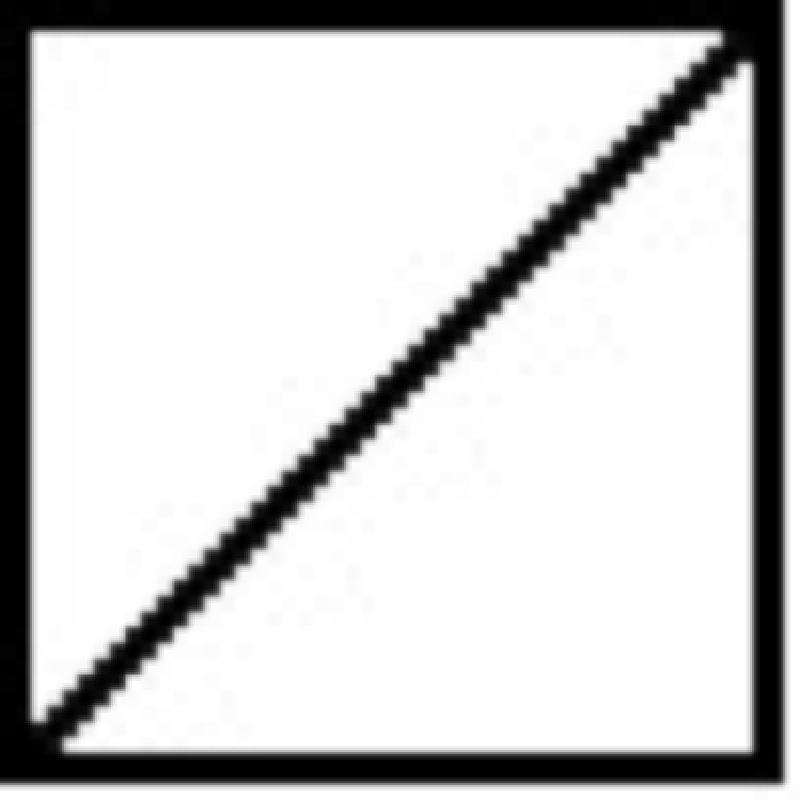
\includegraphics[width=1.7cm]{pictures/wuerf5}\\[7ex]
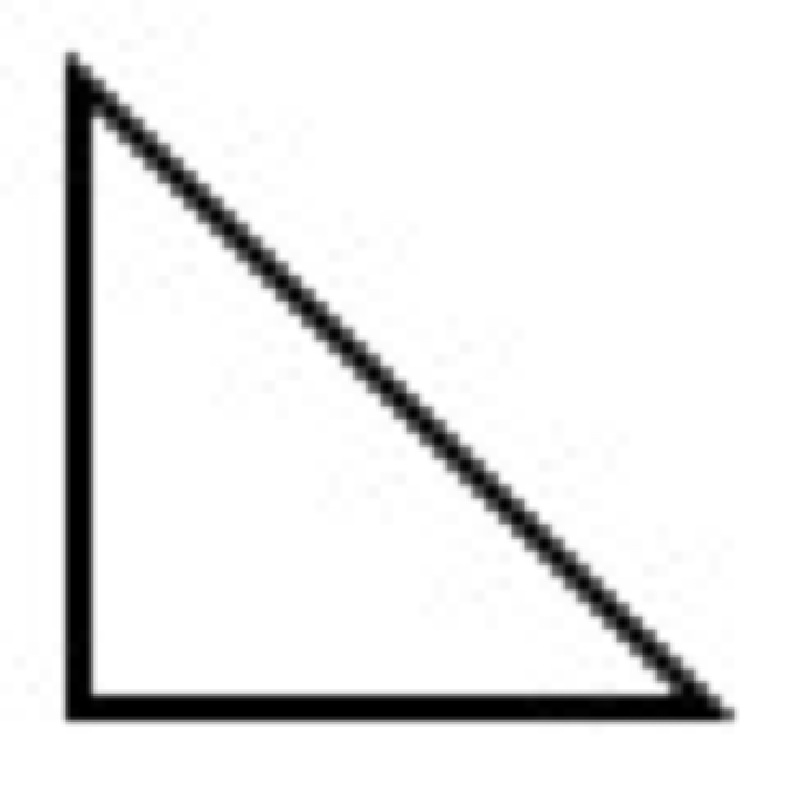
\includegraphics[width=1.7cm]{pictures/wuerf6}
\end{minipage}\\
Bei diesen Operationen hat sich der Wert von $E-K+F=1$ nicht ver\"andert. Ber\"ucksichtigt man noch Punkt 1., so muss f\"ur das Polyeder $E-K+F=2$ gelten.
\end{proof}

\begin{ueb}
Zeichne die entsprechende Beweisfiguren f\"ur das Tetraeder.
\end{ueb}

\begin{ueb}
Ein konvexes Polyeder hat 14 Fl\"achen und 24 Ecken. Wie viele Kanten hat es?
\end{ueb}

\clearpage

\section{Polarkoordinaten}
Die Lage eines Punktes $P$, verschieden von $\point{0}{0}$, in einem rechtwinkligen Koordinatensystem kann nicht nur durch seine kartesischen Koordinaten $\point{x}{y}$, sondern auch durch seinen Abstand $r>0$ vom Ursprung und einem Richtungswinkel $\varphi\in[0,2\pi)$ eindeutig angegeben werden.
\begin{center}\definecolor{qqwuqq}{rgb}{0,0.39,0}
\scalebox{1.1}{
\begin{tikzpicture}[line cap=round,line join=round,>=triangle 45,x=0.5cm,y=0.5cm]
\draw[->,color=black] (-2.78,0) -- (10,0);
\foreach \x in {-2,-1,1,2,3,4,5,6,7,8,9}
\draw[shift={(\x,0)},color=black] (0pt,2pt) -- (0pt,-2pt);
\draw[color=black] (9.66,0.08) node [anchor=south west] {$x$};
\draw[->,color=black] (0,-2.28) -- (0,8.3);
\foreach \y in {-2,-1,1,2,3,4,5,6,7,8}
\draw[shift={(0,\y)},color=black] (2pt,0pt) -- (-2pt,0pt);
\draw[color=black] (0.1,7.9) node [anchor=west] {$y$};
\clip(-2.78,-2.28) rectangle (10,8.3);
\draw [shift={(0,0)},line width=1.6pt,color=qqwuqq,fill=qqwuqq,fill opacity=0.1] (0,0) -- (0:2) arc (0:44.22:2) -- cycle;
\draw [line width=2pt] (5.92,5.76)-- (0,0);
\fill [color=black] (5.92,5.76) circle (1.5pt);
\draw[color=black] (6.2,6.2) node {$P$};
\draw[color=black] (2.76,3.26) node {$r$};
\draw[color=qqwuqq] (1.26,0.5) node {$\varphi$};
\end{tikzpicture}
}
\end{center}

\begin{cdef}[Polarkoordinaten]{}
Das Paar $\point{r}{\varphi}$ nennt man die \emph{Polarkoordinaten} von $P$.
\end{cdef}

\begin{ueb}
Stelle Formeln f\"ur die Umrechnung von kartesischen Koordinaten $\point{x}{y}$ in Polarkoordinaten und vice versa auf.
\end{ueb}

\begin{ueb}
Berechne die Polarkoordinaten der Punkte $K_1=\point{3}{0}$ und $K_2=\point{-3}{-4}$, sowie die kartesischen Koordinaten der Punkte $P_1=\point{7}{\frac{\pi}{2}}$ und $P_2=\point{5}{\frac{7\pi}{4}}$.
\end{ueb} 

\begin{ueb}
Zeichne die Kurven der Gleichungen. Benutze gegebenenfalls eine Wertetabelle.

  \begin{minipage}{3.5cm}
    \begin{enumeratea}
      \item $r=4$
      \item $\varphi=60^\circ$
      \item $r=\cos(2\varphi)$
    \end{enumeratea}
  \end{minipage}
  \begin{minipage}{4cm}
    \begin{enumeratea}\addtocounter{enumi}{3}
      \item $r=10\sin(3\varphi)$
      \item $r=5(1-\cos\varphi)$
      \item $r=4\cos(2\varphi)/\cos\varphi$
    \end{enumeratea}
  \end{minipage}
\end{ueb}

\begin{ueb}
Zeichne die Kurve, die durch folgende Parametergleichung gegeben ist
\begin{align}
x&=2(t-\sin t)\notag\\
y&=2(1-\cos t)\notag
\end{align}
mit $t\in\D{R}$.
Diese Kurve wird als \emph{Helena der Mathematik} bezeichnet.
\end{ueb}

\clearpage
\listoffigures
%\listoftables
%\newpage
%\nocite{*}
%\bibliographystyle{plain}
%\bibliography{preamble/literaturgoogle}
\end{document}